%% Biomimetic Intelligence and Robotics (KeAi/Elsevier) submission version.
%% Content is ported from ../main.tex (IEEEtran); only the front matter,
%% the abstract, the declarations and the class-level formatting differ.
\documentclass[a4paper,fleqn]{cas-dc}

\usepackage[numbers,sort&compress]{natbib}
\usepackage{siunitx}
\usepackage{tabularx}
\usepackage{xurl}   % CAS columns are narrow; allow URL breaks anywhere
\usepackage[protrusion=true,expansion=false]{microtype}
\usepackage{inconsolata}

% Figures live one level up, alongside the IEEEtran source.
\graphicspath{{./}{../}}

\sisetup{
  range-phrase = {\,--\,},
  range-units  = single,
  detect-weight = true,
  detect-family = true,
  separate-uncertainty = true,
}

% Uniform row height for the multi-line table headers used in Section 5.
\renewcommand{\theadfont}{}
\renewcommand{\cellalign}{cc}

% Table notes: \centering (set by the table env) leaves \rightskip/\parfillskip
% at fil, which centres every last line. \tabnote restores normal justification.
% The 2em of \rightskip stretch is not cosmetic: notes carry unbreakable
% \path{} and \texttt{} filenames, and in a full-justified column those force
% badness-10000 underfull lines with visibly gaping interword space. A little
% permitted raggedness absorbs them instead.
% The prose was written against IEEEtran column width; CAS columns are
% narrower, so give the line breaker some slack rather than rewording.
\emergencystretch=3em

% fleqn indents every display by \mathindent; the widest displays here need
% that space back to fit a CAS column.
\setlength{\mathindent}{0pt}

\newcommand{\tabnote}{\par\leftskip=0pt\rightskip=0pt plus 2em%
  \parfillskip=0pt plus 1fil\relax}

% cas-dc leaves LaTeX's stock float parameters in place (topfraction .7,
% textfraction .2, totalnumber 3).  This paper carries 17 tables and 7 figures,
% several taller than 70% of a column, so under the stock values every large
% [t] float is deferred and the whole queue flushes after the bibliography.
% These are IEEEtran's values, which the source document was laid out against.
\setcounter{topnumber}{3}
\setcounter{bottomnumber}{2}
\setcounter{totalnumber}{5}
\setcounter{dbltopnumber}{3}
\renewcommand{\topfraction}{0.9}
\renewcommand{\bottomfraction}{0.7}
\renewcommand{\textfraction}{0.07}
\renewcommand{\floatpagefraction}{0.85}
\renewcommand{\dbltopfraction}{0.9}
\renewcommand{\dblfloatpagefraction}{0.85}

% A float tall enough to claim a column of its own is centred there by LaTeX's
% stock \@fptop/\@fpbot (both 0pt plus 1fil), which opens a gap above *and*
% below it.  Top-align float pages and columns instead, so any slack collects
% in one place at the bottom rather than in two.
\makeatletter
\setlength{\@fptop}{0pt}
\setlength{\@fpsep}{8pt plus 1fil}
\setlength{\@fpbot}{0pt plus 1fil}
\setlength{\@dblfptop}{0pt}
\setlength{\@dblfpsep}{8pt plus 1fil}
\setlength{\@dblfpbot}{0pt plus 1fil}
\makeatother

\begin{document}
\let\WriteBookmarks\relax

\shorttitle{Anchored Conditionally-Gated Control}
\shortauthors{V. T. Nguyen and N. T. Vo}

\title[mode = title]{Anchored Conditionally-Gated Control for Wheeled Bipedal
Balance and Disturbance Recovery}

% Add an ORCID as \author[1]{...}[orcid=0000-0000-0000-0000] and delete the
% \RenewDocumentCommand below; without one the class prints an empty
% "ORCID(s):" footnote.
\RenewDocumentCommand\printorcid{}{}
\author[1]{Van Thuong Nguyen}
\ead{nvthuong180702@gmail.com}
\credit{Conceptualization, Methodology, Software, Validation, Investigation,
Data curation, Writing -- original draft, Visualization}

\author[1]{Nhu Thanh Vo}
\cormark[1]
\ead{vnthanh@dut.udn.vn}
\credit{Conceptualization, Methodology, Validation, Formal analysis,
Investigation, Data curation, Writing -- review and editing, Visualization}

\affiliation[1]{organization={The University of Danang},
            city={Da Nang},
            country={Viet Nam}}

\cortext[1]{Corresponding author.}

\begin{abstract}
Wheeled bipedal robots confront a design trade-off in which the stiffness that
buys precise standing shrinks the push-recovery envelope, while the integral
action that removes equilibrium bias winds up during disturbances. The Anchored
Conditionally-Gated Controller answers both through conditional activation. Its
position integral is confined to a \SI{15}{cm} neighbourhood and enabled by an
asymmetric envelope follower whose \SI{23}{ms} attack and \SI{1.5}{s} release
separate quiet stance from post-push ringdown. On a \num{10}-DOF, \SI{8.1}{kg}
wheeled biped in MuJoCo the architecture is dissected rather than merely
demonstrated. A factorial ablation separates three coupled effects. Gated
damping produces the steadiness, the anchor integral produces the accuracy at a
threefold cost in steadiness, and the gates are bit-for-bit inert in quiet
stance yet decisive under disturbance. The push envelope is measurably chiral at
\SI{-17.3}{N}, traced to the antisymmetric hip-roll and hip-yaw sign convention
and closed by two controls, since a mirror flips the asymmetry and a sham mirror
does not. A closed-form model predicts the \SI{27.0}{mm} standing offset to
\SI{0.92}{\percent} across a fortyfold gain sweep and identifies it as the price
of a bounded integrator memory. ACC holds $0.294{\pm}0.015$\,mm sagittal
repeatability over ten trials, a \num{59}-fold improvement on the
proportional-only rung of the same ablation, recovers omnidirectional pushes at
\SI{108}{N} median and \SI{82}{N} worst case, stands \SI{30}{min} at
\SI{0.0004}{mm/min} drift where six classical baselines and a full-state LQR all
fall, and survives a \SI{100}{cm} drop as well as curbs of
\SIrange{10}{20}{cm}. A \SI{2}{ms}-resolved delay screen prices deployment at a
latency cliff of \SIrange{6}{8}{ms} that a single retuned gain moves outward,
making the cliff a tuning artefact rather than an architectural ceiling.
\end{abstract}

\begin{highlights}
\item Gated damping delivers the steadiness while the anchor integral delivers accuracy.
\item A chiral push envelope is traced to a sign convention and closed by mirror controls.
\item Closed-form model predicts the 27 mm standing offset to 0.92\% over a 40x sweep.
\item 0.294 mm standing repeatability, held as a fixed point for 30 min without falling.
\item Recovers 108 N median pushes, a 100 cm free fall, and 10-20 cm curbs per-leg.
\end{highlights}

\begin{keywords}
Wheeled biped robot \sep Conditionally-gated control \sep Anchored standing \sep
Proximity-gated integral \sep Push recovery \sep Terrain adaptation
\end{keywords}

\maketitle

\printcredits

\section{Introduction}
\label{sec:intro}
% ============================================================

Wheeled biped robots are expected to stand with millimetre precision, to survive
pushes from any direction, and to adapt to uneven ground, yet no single
classical controller delivers all three at once. LQR is the usual answer for
balance~\cite{klemm2019ascento}, whole-body control for
posture~\cite{klemm2020lqrwbc} and MPC for terrain~\cite{skater2024}, while
locomotion is reached for separately again through learned
policies~\cite{hwangbo2019rl}.

The obstacle is structural rather than a matter of tuning. Lowering the
proportional gain widens the capture basin at the cost of balance stiffness, and
omitting integral action leaves a \SI{1.3}{Nm} equilibrium bias that sustains a
persistent limit cycle whatever that gain is set to, a cycle that is
predominantly sagittal at \SI{69.7}{mm} peak to peak along the rolling direction
against \SI{13.4}{mm} laterally. It lives on the one axis the wheels can drive,
which is both why it persists and why every mechanism developed here is aimed at
it, and restoring a global integral removes the bias but winds up during a push,
so the two obvious remedies exclude one another.

This paper presents the Anchored Conditionally-Gated Controller, which resolves
both dilemmas through conditional activation. Its central mechanism is a
proximity-gated anchor, a position integral confined to a \SI{15}{cm}
neighbourhood of the commanded home and enabled by an asymmetric envelope
follower whose \SI{23}{ms} attack and \SI{1.5}{s} release distinguish quiet
stance from post-push ringdown. Coupled with a gated damping boost, ACC reaches
$0.294{\pm}0.015$\,mm repeatability on the sagittal axis under clean sensing
and zero actuator delay over ten trials, at push performance equal to or better
than the proportional-only rung that carries no integral action at all.
Absolute accuracy on that axis is a separate quantity. The robot parks
\SI{27.0}{mm} from the commanded home and then holds that offset to
\SI{0.009}{mm}, a behaviour measured in Section~\ref{sec:standing} and derived
in closed form in Appendix~\ref{sec:parking_supp}.

A factorial ablation run under a single protocol, reported in
Table~\ref{tab:standing}, locates the mechanism more precisely than the gate
structure alone would suggest. Quiet-stance steadiness comes from the gated
damping terms rather than from the anchor integral, since disabling the integral
while leaving every gate intact improves sagittal repeatability from
\SI{0.294}{mm} to \SI{0.089}{mm} whereas reverting the two velocity-damping
coefficients reinstates the full \SI{25.2}{mm} limit cycle. What the integral
buys is accuracy, removing \SI{4.2}{mm} of sagittal parking offset at a threefold
cost in steadiness, and because the two properties come from different mechanisms
and trade against each other they are reported as separate columns rather than as
a single planar number. The proximity gate and the asymmetric envelope are by
contrast inert during quiet stance, ablating either reproducing ACC bit for bit
because the robot never leaves the gate's inner band nor the envelope's release
branch while standing still, so their contribution is windup prevention and
ringdown control that only a displacement experiment can measure. The pitch
safety gate is load-bearing even with no disturbance applied and removing it
produces divergence from initial-condition noise alone in all ten trials. The
gates are therefore enabling conditions that make an otherwise inadmissible
damping and integral configuration safe, rather than the proximate source of the
precision.

Against that architecture we place six classical baselines, four derived from a
4-state TWIP model and two from a 6-state coupled model, all of which fall in
every trial, removing the PID servo path in the direct-torque variant buying only
\SI{0.28}{s} of survival at an unchanged fall rate. A seventh design, a
full-state LQR linearized from the plant itself, removes the model-mismatch
objection in Section~\ref{sec:full_state_lqr} and survives two orders of
magnitude longer while still falling, so platform complexity rather than model
order or servo lag dominates the failure.

The work is positioned within structured classical priors rather than within
learned control, its object of study being a hand-designed and fully
interpretable torque assembly whose gating encodes the plant's measured failure
modes explicitly. It was built to serve as the nominal base action of a
residual-learning stack, where a policy corrects a structured prior instead of
searching the space unaided~\cite{johannink2019residual,silver2018residual}, and
that origin explains its shape, since such a prior wants to be interpretable,
bounded and gated rather than optimal. What the paper reports is the prior
itself, no residual policy being trained here, so the classical controllers are
the comparison of record. A preliminary PPO~\cite{schulman2017ppo} run of 5.4M
steps on a single seed motivates the structure without bounding it, standing at
one height for about \SI{3.20}{s} against \SIrange{0.16}{0.60}{s} for the
classical baselines but failing to generalize across the
\SIrange{0.40}{0.70}{m} base-$z$ range of Section~\ref{sec:height_convention},
with height RMSE above \SI{50}{mm} and falls on \SI{85}{\percent} of squat
transitions. Those failures concentrate on exactly the coupled pitch and height
dynamics that a posture map and a gate schedule encode explicitly, and since the
run is single-seed and carries neither domain
randomization~\cite{tobin2017domainrand,peng2018dynrand} nor a hyperparameter
search it is retained as a difficulty probe rather than as a bound.

The contributions are threefold. First, a proximity-gated anchor with an
asymmetric envelope follower attains sub-millimetre idle precision without
sacrificing omnidirectional push survival. Second, a two-channel
conditionally-gated torque assembly carries flight recovery and per-leg terrain
adaptation as independent extensions, each ablated to establish which mechanism
is necessary for which behaviour, with thirty repetitions on push and ten on
idle and terrain. Third, a factorial ablation combining an additive ladder
L0--L3 with a subtractive ladder S0--S5 is run against the six classical
baselines and supplemented by two control experiments that test the comparison
itself, namely a full-state LQR derived from the plant rather than from a
reduced model and a sweep of the coupled model's single empirical constant.

The remainder of the paper is organized as follows.
Section~\ref{sec:related} reviews wheeled bipedal control and the
disturbance-rejection literature ACC departs from, Section~\ref{sec:platform}
describes the robot and the simulation setup and Section~\ref{sec:formulation}
develops the controller. Section~\ref{sec:results} reports the experimental
validation, from anchored standing through push, flight, terrain, baseline
comparison and architectural analysis, and Section~\ref{sec:discussion} states
the limitations and the deployment consequences that follow from them, with three
appendices supplying the anti-windup argument, the whole-body control baseline
details and the closed-form account of the standing offset.


% ============================================================
\section{Related Work}
\label{sec:related}
% ============================================================

\subsection{Wheeled Bipedal Platforms and Classical Control}
\label{sec:related_pos}
Ascento~\cite{klemm2019ascento} demonstrated two-wheeled jumping under LQR
balancing and was later extended to whole-body control with kinematic
loops~\cite{klemm2020lqrwbc}. Handle~\cite{boston_dynamics_handle2017} pioneered
wheeled-leg coordination, and wheeled quadrupeds combined driving with walking
through whole-body motion control and planning~\cite{bjelonic2019wheeled}.
Ollie~\cite{zhang2022ollie} adapts whole-body balance control to a two-wheeled
biped, while wheeled quadrupeds have since been driven by whole-body MPC with
online gait sequencing~\cite{bjelonic2021mpc}. DIABLO~\cite{diablo2024} pairs an
LQR balance controller with separate yaw, split-angle, height and roll loops,
and SKATER~\cite{skater2024} uses a hierarchical MPC whole-body controller with
centrifugal-force compensation and terrain adaptation. Closest to our morphology
is Whleaper~\cite{whleaper2024}, which also carries ten degrees of freedom with
three hip axes per leg. It applies LQR to balanced sliding and a separately
trained PPO policy to walking, switching between the two by locomotion mode
rather than composing them on a shared control output. Composing a classical
prior with a learned residual on one output is instead the residual-RL
construction~\cite{johannink2019residual,silver2018residual}, applied recently
to wheeled-biped balance~\cite{zhang2025residualwbr}, and ACC is designed to
supply the classical prior in that construction rather than to replace the
learned part. Placing ACC beside these platforms on the capabilities measured here is
possible only in a limited sense, because none of the cited works reports idle
standing precision, a quantitative push threshold or a per-leg terrain estimate,
their balance layers being LQR on Ascento, LQR with auxiliary loops on DIABLO,
mode-switched LQR and PPO on Whleaper and hierarchical MPC with vision-based
terrain adaptation on SKATER. The one comparison that runs cleanly in the other
direction is validation, since all four are demonstrated on hardware whereas
every result here is in simulation.

Coupled pitch--roll LQR is standard on rigid two-wheeled platforms, where torque
acts directly on the wheels and there are neither articulated legs nor
leg-height dynamics, which makes for a structurally simpler problem with fewer
unstable modes. Our 6-state LQR reproduces that coupled structure on a legged
morphology and fails, and the 4-state direct-torque variant, which removes the
servo path and re-optimizes the roll gain to $k_{p,\text{roll}}{=}55.0$, fails as
well at a full fall rate and \SI{0.60}{s} of survival. Since that variant carries
no servo lag whatsoever and still falls, as Section~\ref{sec:baselines} shows,
actuation lag alone cannot account for the outcome and the articulated-leg
morphology with its height dynamics is the dominant remaining factor. Both
variants take their gains from a simplified 4-state TWIP model rather than from a
full 10-DOF linearization, an objection removed by the control experiment of
Section~\ref{sec:full_state_lqr}.

Cascade control~\cite{cascade_standard} and whole-body control through
hierarchical inverse dynamics or task-priority quadratic
programs~\cite{herzog2016wbc,bellicoso2018wbc,escande2014hqp} use fixed-gain
nested or strictly prioritized loops without conditional gates, while gain
scheduling~\cite{gain_scheduling_survey,leith2000gainsched} varies parameters
continuously with one scheduling variable rather than responding to
qualitatively distinct physical regimes. We benchmarked a task-priority QP
whole-body controller both standalone and as an assist layer on ACC in
Section~\ref{sec:wbc}, where it fails to resolve the precision and recovery
trade-off because its fixed formulation carries no conditional regime gating.
Split-range, selector and override
architectures~\cite{shinskey1996,astrom2005advanced} already implement continuous
blending in process control and ACC adopts that principle, its contribution being
the synthesis of physically motivated gating surfaces, one spatial in proximity,
one temporal in the velocity envelope and one a pitch safety interlock, derived
from wheeled-biped failure modes rather than from generic process-variable
limits. The gates also connect ACC to hybrid and switched
systems~\cite{liberzon2003switching} and to hysteresis-based switching
logic~\cite{hespanha2003hysteresis}, which deliberately breaks the symmetry of a
switching surface to prevent chattering, an asymmetry ACC realizes in continuous
time through its fast-attack and slow-release envelope with smoothstep softening
the surfaces to $C^1$ transitions. Section~\ref{sec:stability} makes that
connection quantitative by locating the operating point relative to every
switching surface and settling the one switch that does fire with a common
Lyapunov function. A recent review~\cite{liu2024review} surveys wheel-legged
biped platforms and notes the absence of a unified classical solution.

\subsection{Disturbance Rejection, Anti-Windup, and ACC's Distinction}
Disturbance observers~\cite{ohnishi1993dob,chen2000dob} and active disturbance
rejection~\cite{han2009adrc,feng2023lqradrc} provide temporal disturbance
estimation but cannot distinguish a push from the ringdown that follows it,
because both occupy the same frequency band. Classical anti-windup in its
back-calculation, conditional-integration and unified observer-based
forms~\cite{astrom1989windup,kothare1994antiwindup,tarbouriech2009aw} triggers on
actuator saturation, whereas ACC's anchor gates spatially and on physics. The
proximity gate confines integration to a \SI{15}{cm} neighbourhood and the
asymmetric envelope separates quiet stance from ringdown by velocity envelope,
which replaces the estimation-speed against noise trade-off with a time-domain
attack against release trade-off. Push recovery through capture
point~\cite{englsberger2015dcm,pratt2006capturepoint} and flight-phase
control~\cite{roscia2023flight} is complementary, and blind stair climbing by
reinforcement learning has been shown on Ascento~\cite{chamorro2024stairclimbing}.
Terrain adaptation is usually built on exteroceptive elevation
mapping~\cite{legged_terrain_extero,fankhauser2018rough}, on learned policies
that fuse proprioception with terrain
estimates~\cite{lee2020challenging,miki2022perceptive}, or on purely
proprioceptive contact
sensing~\cite{blind_terrain_proprio,bellicoso2016terrain,camurri2017contact},
and ACC extends proprioceptive contact-point estimation to wheeled bipeds.
Hyon and Cheng~\cite{hyon2007gated} achieved full-body humanoid balancing by
gravity compensation with optimal contact-force distribution, making the robot
passive to external forces without measuring them. ACC shares the requirement of
reacting to unmeasured pushes but meets it by switching regime on proprioceptive
gating variables rather than by redistributing contact forces.

% ============================================================
\section{Robot Platform}
\label{sec:platform}
% ============================================================

\subsection{Robot Morphology and Simulation}
The robot shown in Fig.~\ref{fig:robot} is a ten-DOF wheeled biped carrying five
actuated joints per leg, namely hip roll, hip yaw, hip pitch, knee and drive
wheel. It has a mass of \SI{8.1}{kg}, a \SI{0.26}{m} thigh, a \SI{0.28}{m}
shin, wheels of \SI{0.06}{m} radius and a hip width of \SI{0.23}{m}. Torque is
limited to \SI{30}{Nm} on the hip-roll, hip-yaw and wheel axes and to
\SI{150}{Nm} on hip pitch and knee.

Simulation runs in MuJoCo~\cite{mujoco} at \SI{500}{Hz}. ACC and every classical
baseline are controlled at \SI{100}{Hz} over five physics substeps, the classical
baselines are additionally measured at their \SI{50}{Hz} design rate in
Section~\ref{sec:rate_matched}, and the PPO reference is reported at the
\SI{50}{Hz} rate it was trained at, with a \SI{400}{Nm/s} torque rate limit and
raw torque commands throughout. The integrator is implicitfast with four solver
and eight linesearch iterations, the friction cone is pyramidal for the body and
elliptic for the wheels with $\mu_s{=}1.2$ and $\mu_k{=}0.8$, armature is
\SI{0.008}{kg{\cdot}m^2} on the wheels and \SI{0.02}{kg{\cdot}m^2} on the leg
joints, and contact stiffness follows \texttt{solref}=\{0.002,1\} on the body and
\{0.005,0.7\} on the wheels. That stiff body contact idealizes rigid ground, and
softening \texttt{solref[0]} to \num{0.02}, which approximates tire on asphalt,
raises planar idle RMS by roughly \SI{60}{\percent} to about \SI{1.2}{mm}, so
every sub-millimetre idle figure reported here is conditional on stiff ground
contact.

\subsubsection*{Height convention}
\label{sec:height_convention}
Two vertical references appear in this paper and are easily confused, so we fix
them here and mark every height accordingly. CoM-$z$ is the height of the
whole-body centre of mass above ground and is the quantity ACC commands and
regulates, with the nominal standing pose at $h_{\text{CoM}}{=}\SI{0.404}{m}$,
whereas base-$z$ is the torso root-body height \texttt{qpos[2]} in the MuJoCo
model, at which the same pose sits at $z_{\text{base}}{=}\SI{0.536}{m}$,
\SI{13.2}{cm} above the centre of mass. The offset is pose-dependent but varies
by less than \SI{1}{cm} over the postures used here. All ACC results are reported
in CoM-$z$, whereas the PPO reference of Section~\ref{sec:baselines} commands
base-$z$ over \SIrange{0.40}{0.70}{m} and the WBC baselines of
Section~\ref{sec:wbc} inherit that convention, so those numbers are labelled
base-$z$ where they appear and must not be compared numerically against CoM-$z$
heights, substituting one for the other in a height command injecting the full
\SI{13.2}{cm} offset as a reference error.

ACC's posture map is calibrated at two setups, at CoM heights of \SI{0.354}{m}
and \SI{0.454}{m} ($\pm\SI{5}{cm}$ about nominal), and interpolated between
them. Outside that band the joint targets are linearly extrapolated, bounded to
the interval $[0.254, 0.554]\,$m, i.e.\ \SI{10}{cm} beyond the calibrated band at
each end. This $\pm\SI{10}{cm}$ extrapolation bound, and not a $\pm\SI{5}{cm}$
one, is what the per-leg height split (Section~\ref{sec:terrain}) operates against.

\begin{figure}[pos=t]
    \centering
    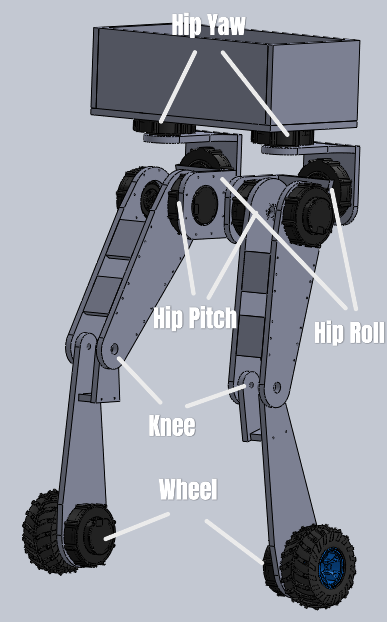
\includegraphics[width=\linewidth]{figures/annotated_robot_joints.png}
    \caption{Robot joint layout with world coordinate frame (right-handed, Z up). In the model as built, both wheel axles lie along world $X$ and the two wheel links are separated by \SI{0.271}{m} along $X$; the rolling (and therefore sagittal) direction is world $Y$, and world $X$ is the lateral (track) axis. All axis-resolved results in this paper follow that convention, verified four independent ways in Section~\ref{sec:standing}. The CoM is located at the torso geometric center. Each leg: hip roll (HR), hip yaw (HY), hip pitch (HP), knee (KN), wheel (WH).}
    \label{fig:robot}
\end{figure}

% ============================================================
\section{ACC Formulation}
\label{sec:formulation}
% ============================================================

\subsection{Two-Channel Torque Assembly}
\label{sec:overview}

ACC assembles a PD balance core, a proximity-gated anchor integral and posture
regulation into two torque channels, the wheel torque
$\boldsymbol{\tau}_w\in\mathbb{R}^2$ and the leg-joint torque
$\boldsymbol{\tau}_q\in\mathbb{R}^8$, with flight and terrain entering as
independent extensions as sketched in Fig.~\ref{fig:acc_arch},

\begin{equation}
\begin{aligned}
\boldsymbol{\tau}_w &= (1-g_{\text{flight}})\!\big[\boldsymbol{\tau}_{\text{balance}} + g_{\text{anchor}}\boldsymbol{\tau}_{\text{anchor}}\big] + g_{\text{flight}}\boldsymbol{\tau}_{\text{flight}},\\
\boldsymbol{\tau}_q &= \boldsymbol{\tau}_{\text{posture}}\big(h^{\text{cmd},L},\,h^{\text{cmd},R}\big) + \boldsymbol{\tau}_{\text{lat}} + \boldsymbol{\tau}_{\text{yaw}}.
\end{aligned}
\label{eq:two_channel}
\end{equation}

Two structural points are easy to misread as sums. The flight term is an override
rather than a summand, so at $g_{\text{flight}}{=}1$ it replaces the wheel torque
instead of adding to it, a deliberate replacement since the balance core
regulates sagittal position and velocity against a ground that unloaded wheels do
not have, while the convex blend makes the substitution continuous. Per-leg
ground adaptation likewise enters as a reference split rather than as an extra
torque, the posture regulator always taking two height commands that coincide on
level ground and separate through Eq.~\eqref{eq:terrain_split} across a step,
while the gate $g_{\text{terrain}}$ appears not in $\boldsymbol{\tau}_q$ but in
the wheel channel, where it retunes the sagittal loop for the straddle treated in
Section~\ref{sec:terrain}.

Every gate $g_*$ except the flight gate is a smoothstep function of a physical
condition such as proximity, quietness, attitude or terrain disparity rather
than a discrete switch,

\begin{equation}
\operatorname{ss}(x;a,b) = 3t^2 - 2t^3,
\qquad t = \operatorname{clip}\!\left(\frac{x-a}{b-a},\,0,\,1\right).
\label{eq:smoothstep}
\end{equation}

Equation~\eqref{eq:smoothstep} is the standard Hermite blend, $C^1$ in $x$, equal
to zero for $x\leq a$ and to one for $x\geq b$, with vanishing derivative at both
knees. Continuity matters for a concrete reason, because a hard threshold on any
of these conditions injects a torque step whose magnitude equals the full gated
component, and at \SI{100}{Hz} under a \SI{400}{Nm/s} rate limit the rate limiter
spreads that step over several control cycles and delivers it to the plant as an
unmodelled impulse. Smoothstep removes the step entirely and the rate limiter is
therefore never the active constraint during a gate transition. The one exception
is $g_{\text{flight}}$, and only on the way in, since contact loss is a binary
physical event, so engagement is a latched load-based hysteresis that arms after
two consecutive steps with both wheels unloaded and releases after five steps at
$F_z \geq 0.5mg$, an asymmetry that exists specifically to prevent balance torque
from re-engaging during landing bounce. The handback is not discrete either,
$g_{\text{flight}}$ ramping linearly to zero over fifteen steps after release,
because an instant handback at large pitch would return roughly \SI{19}{Nm} of
wheel authority to a marginally loaded wheel and re-launch the robot. One caveat
applies to the composition
$g_{\text{env}} = 1 - \operatorname{ss}(\mathrm{EMA}(|v_{\text{sag}}|);\cdot)$,
which is only $C^0$ in time because the asymmetric EMA of
Eq.~\eqref{eq:asym_ema} switches coefficients when $|v_t|$ crosses
$\mathrm{EMA}_{t-1}$. The smoothstep remains $C^1$ in its argument, so the
resulting torque is continuous while its time derivative may jump at an attack
or release transition.

Wheel torques control sagittal balance, whereas lateral and yaw regulation sense
torso state but actuate in the leg-joint channel through the antisymmetric
hip-roll and hip-yaw pairs of Eq.~\eqref{eq:lat_yaw}, so the wheels carry no roll
or yaw differential. On level ground the two channels are coupled only through
the plant, since with $h^{\text{cmd},L}{=}h^{\text{cmd},R}$ the terrain gate is
identically zero and no term in $\boldsymbol{\tau}_w$ reads a leg-posture state.
Across a step the gate becomes a function of
$|h^{\text{cmd},L}-h^{\text{cmd},R}|$ and reaches into the wheel channel in four
places, softening $k_{\text{pos}}$, raising the position-torque cap, adding a
pitch-rate feedforward to the wheel-velocity setpoint and symmetrising the
per-wheel damping so that a one-wheel step is not read as a yaw command, a
coupling confined to the straddle and vanishing continuously with the height
split, which is what allows the extensions of Sections~\ref{sec:flight}
and~\ref{sec:terrain} to be added without retuning the anchor.

Conditional gating here denotes smoothstep activation by physical conditions,
namely $g_{\text{prox}}$, $g_{\text{env}}$, $g_\theta$ and $g_{\text{terrain}}$,
and it differs from the industrial override architectures of
Section~\ref{sec:related_pos} in gating components within a single torque
assembly by physical regime rather than selecting among parallel controllers by
process-variable limits. The gating variables are not control errors but physical
quantities of three different kinds, one spatial, one temporal and one a safety
interlock on attitude, each chosen because a specific measured failure mode of
this platform is expressible in it.

\begin{figure}[pos=!htbp]
    \centering
    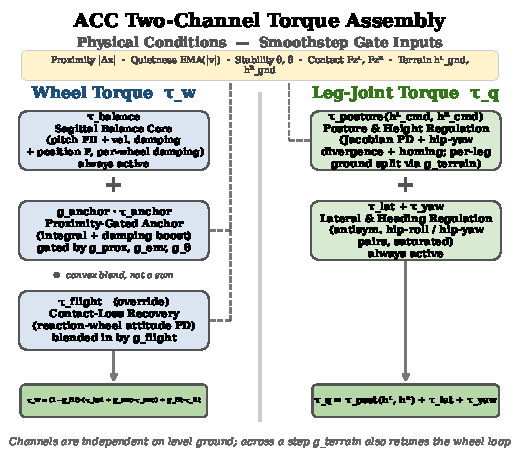
\includegraphics[width=\linewidth]{figures/acc_architecture.pdf}
    \caption{ACC two-channel torque assembly. Physical conditions gate each component via continuous smoothstep functions (dashed). The flight gate is the one latched exception, and it \emph{overrides} the wheel channel rather than adding to it; per-leg ground adaptation enters the posture regulator as a split pair of height references, not as an added torque.}
    \label{fig:acc_arch}
\end{figure}

\subsection{Sagittal Balance Core ($\boldsymbol{\tau}_{\text{balance}}$)}
\label{sec:balance_core}

The sagittal balance component is always active and acts entirely in the
wheel-torque channel,

\begin{equation}
\boldsymbol{\tau}_{\text{balance}} =
\begin{bmatrix}
\tau_{\text{com}} + \tau_{w}^{L} \\
\tau_{\text{com}} + \tau_{w}^{R}
\end{bmatrix},
\quad
\begin{aligned}
\tau_{\text{com}} &= \tau_{\text{pitch}} + \tau_{\text{damping}} + \tau_{\text{pos}},\\
\tau_{w}^{i} &= -k_{w}\big(\omega^{i} - \omega^{\text{cmd}}\big).
\end{aligned}
\label{eq:balance}
\end{equation}

where $\tau_{\text{com}}$ is the common-mode balance torque, identical on both
wheels, and $\tau_{w}^{i}$ for $i\in\{L,R\}$ is the per-wheel velocity damping
toward the commanded wheel speed, the only term that differs between the two
wheels. The individual terms are

\begin{align}
\tau_{\text{pitch}} &= k_p\cdot\theta + k_d\cdot\dot{\theta},\\
\tau_{\text{damping}} &= -\big(s_v k_{\text{vel}} + k_{v2}\big)\cdot v_{\text{sag}},\\
\tau_{\text{pos}} &= -k_{\text{pos}}\cdot\operatorname{clip}(\Delta x,\,\pm\SI{0.10}{m}),
\end{align}

where $\theta$ is the torso pitch angle, $\dot{\theta}$ the pitch rate,
$v_{\text{sag}}$ the sagittal body velocity and $\Delta x$ the sagittal position
error from the latched home position. Two coefficients damp $v_{\text{sag}}$,
the scheduled term $s_v k_{\text{vel}}$ whose scale $s_v$ the M2 and M3
ablations of Section~\ref{sec:idle_mechanism} revert, and a fixed offset
$k_{v2}$ that is never scheduled or gated.

Lateral and yaw regulation read torso state alongside the balance core but
actuate in the leg-joint channel, antisymmetrically across the hip-roll pair
$(\mathrm{HR}^L,\mathrm{HR}^R)$ and the hip-yaw pair
$(\mathrm{HY}^L,\mathrm{HY}^R)$,

\begin{equation}
\begin{aligned}
\boldsymbol{\tau}_{\text{lat}} &=
\begin{bmatrix} +1 \\ -1 \end{bmatrix}
\big(k_{p,\text{roll}}\phi + k_{d,\text{roll}}\dot{\phi}\big),\\[2pt]
\boldsymbol{\tau}_{\text{yaw}} &=
\begin{bmatrix} -1 \\ +1 \end{bmatrix}
\big(k_{p,\text{yaw}}e_\psi - k_{d,\text{yaw}}\omega_z\big),
\end{aligned}
\label{eq:lat_yaw}
\end{equation}

each saturated at its own moment limit, with $\phi$ the roll angle, $e_\psi$ the
yaw error and $\omega_z$ the yaw rate. On this morphology the lateral axis is
closed by the legs rather than by a wheel differential. It is the axis on which
six classical baselines fail in Section~\ref{sec:baselines}, and the fixed sign
pattern of these two antisymmetric pairs is the mechanism behind the chirality
of the push envelope reported in Section~\ref{sec:push}.

The proportional position term, clipped to $\pm\SI{0.10}{m}$ and saturating at
$\pm\SI{4}{Nm}$, keeps the robot within \SIrange{4}{6}{cm} of home but leaves a
\SI{1.3}{Nm} equilibrium bias that sustains a perpetual limit cycle, which is
what motivates the anchor integral. Classical anti-windup does not address it,
because such schemes fire on actuator saturation whereas the critical failure on
this platform is state-dependent, the position error growing to
\SIrange{10}{30}{cm} during a push while the wheels stay well inside their
\SI{20}{rad/s} range, so a saturation-triggered scheme never activates at all.
ACC's proximity gate supplies spatial confinement through a continuous smoothstep
instead, avoiding both the over-restriction that would block slow-drift
correction and the under-restriction that would allow windup during sustained
pushes; the simplest conditional-integration variant is evaluated in
Appendix~\ref{sec:aw_supp} and broader anti-windup families remain open. Pitch
stiffness itself is fixed at $k_p{=}50$, since the anchor and boost resolve the
precision and push trade-off without gain scheduling, and a scheduled variant
softening $k_p$ from \num{50} to \num{35} during pushes was tested and rejected
because it did not improve push survival when S0 and S1 are compared in
Table~\ref{tab:push_ablation}.

\subsection{Proximity-Gated Anchor Mechanism ($g_{\text{anchor}}\!\cdot\!\boldsymbol{\tau}_{\text{anchor}}$)}
\label{sec:anchor}

The anchor mechanism is the core contribution. It adds three terms to the
wheel-torque channel which are active only when the robot is near home and
genuinely at rest,

\begin{equation}
\begin{split}
\boldsymbol{\tau}_{\text{anchor}} = {}
& K_i\!\int\! g_{\text{prox}}\cdot g_{\text{env}}\cdot(-\Delta x)\,dt\\
& + g_{\text{boost}}\cdot K_{\text{boost}}\cdot(-v_{\text{sag}})\\
& + \bigl(k_{d,h}g_h + k_{d,a}g_{\text{prox}}\bigr)g_{\dot{\theta}}\cdot(-\dot{\theta}),
\end{split}
\label{eq:anchor}
\end{equation}

where every gate is a continuous smoothstep designed to equal one when the robot
is at home and quiet and to fall smoothly to zero otherwise,

\begin{align}
g_{\text{prox}}(\Delta x) &= 1 - \operatorname{ss}\bigl(|\Delta x|;\;\SI{0.05}{m},\,\SI{0.15}{m}\bigr),
\label{eq:g_prox}\\[2pt]
g_{\text{env}}(v_{\text{sag}}) &= 1 - \operatorname{ss}\bigl(\mathrm{EMA}(|v_{\text{sag}}|);\;\SI{0.25}{m/s},\,\SI{0.50}{m/s}\bigr),
\label{eq:g_env}\\[2pt]
g_\theta(\theta,\dot{\theta}) &= \bigl[1 - \operatorname{ss}(|\theta|;\,\SI{2}{\degree},\,\SI{12}{\degree})\bigr] \nonumber\\
&\quad\times \bigl[1 - \operatorname{ss}(|\dot{\theta}|;\,\SI{2}{\degree/s},\,\SI{15}{\degree/s})\bigr],
\label{eq:g_theta}\\[2pt]
g_h(\Delta h) &= 1 - \operatorname{ss}\bigl(|\Delta h|;\;\SI{0.05}{mm},\,\SI{0.30}{mm}\bigr),
\label{eq:g_h}\\[2pt]
g_{\dot{\theta}}(\dot{\theta}) &= \operatorname{ss}\bigl(|\dot{\theta}|;\,\SI{2}{\degree/s},\,\SI{15}{\degree/s}\bigr),
\label{eq:g_thetadot}\\[2pt]
g_{\text{boost}} &= g_{\text{prox}}\cdot g_{\text{env}}\cdot g_\theta,
\label{eq:g_boost}
\end{align}

where $\operatorname{ss}(x;a,b)$ denotes the smoothstep of
Eq.~\eqref{eq:smoothstep} with lower and upper knees $a$ and $b$, so each gate is
dimensionless, monotone and $C^1$, equal to one inside its home-and-quiet band
and falling smoothly to zero outside it. Three physically distinct conditions
must therefore hold at once for the anchor to integrate, the robot being
spatially near home through $g_{\text{prox}}$, temporally quiet through
$g_{\text{env}}$ and attitudinally settled through $g_\theta$. The pitch
stability gate closes when either pitch or pitch rate leaves its band, which
prevents the damping boost from fighting a gentle sustained push that never
triggers the velocity envelope, and saturates at one when the robot is genuinely
at rest. The third anchor term is a gated pitch-rate term whose gate
$g_{\dot{\theta}}$ is the complement of the rate factor in $g_\theta$, so it
contributes nothing in quiet stance and engages only once the pitch rate leaves
that band while the robot is still near home and still tracking its commanded
height, applied common-mode to both wheels.

Reliable quiet-stance detection rests on an asymmetric exponentially weighted
moving average of $|v_{\text{sag}}|$,
\begin{equation}
\text{EMA}_t = \begin{cases}
\alpha_a|v_t| + (1{-}\alpha_a)\text{EMA}_{t-1}, & \text{if } |v_t| > \text{EMA}_{t-1},\\
\alpha_r|v_t| + (1{-}\alpha_r)\text{EMA}_{t-1}, & \text{otherwise},
\end{cases}
\label{eq:asym_ema}
\end{equation}
whose primary specification is the pair of time constants
$\tau_{\text{attack}}{\approx}\SI{23}{ms}$ and
$\tau_{\text{release}}{\approx}\SI{1.5}{s}$. The discrete coefficients follow
from $\alpha_a=1-\exp(-\Delta t / \tau_{\text{attack}})\approx 0.35$ and
$\alpha_r=1-\exp(-\Delta t / \tau_{\text{release}})\approx 0.007$ at
\SI{100}{Hz}. The asymmetry is essential because a symmetric EMA is bistable, post-push
oscillation holding it in a middle band where the gate stands half open and the
boost cannot collapse the cycle, an outcome confirmed by the symmetric-EMA
ablation of Section~\ref{sec:results}. The fast-attack and slow-release envelope
instead rises to one only when oscillation truly decays and falls to zero within
roughly \SI{25}{ms} of a disturbance. The mechanism is a peak-hold envelope
detector with asymmetric time constants, and ACC's contribution is to couple that
detector to a spatial proximity gate for integral conditioning, the complete
activation sequence through a push-recovery cycle being shown in
Fig.~\ref{fig:gate_activation}. One implementation detail follows from it,
namely that starting the envelope at zero biases $g_{\text{env}}$ toward one for
about \SI{7.5}{s} before velocity noise accumulates and the bias decays, so
measurements allow \SIrange{3}{5}{s} of settling and a hardware implementation
should initialize the envelope at unity instead.

\begin{figure*}[pos=!tp]
    \centering
    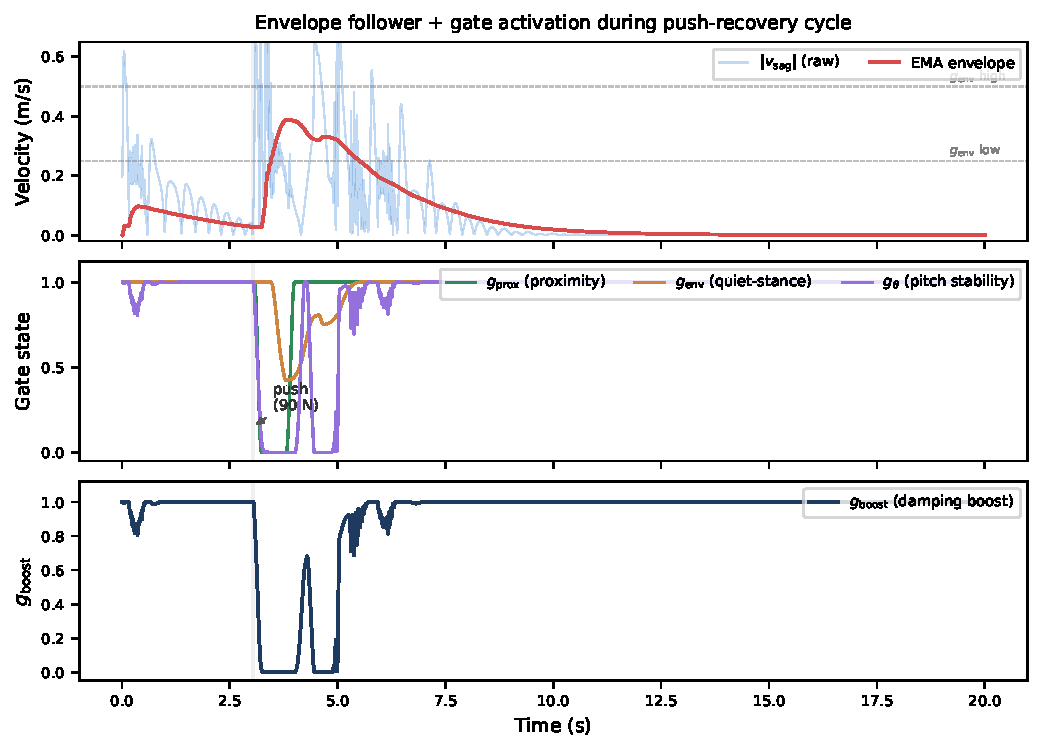
\includegraphics[width=\linewidth]{figures/gate_activation.pdf}
    \caption{Gate activation during a \SI{90}{N} lateral (world $+x$) push-recovery cycle (\SI{100}{Hz} control). \textbf{Top:} $|v_{\text{sag}}|$ and asymmetric EMA envelope; dashed lines mark the \SIrange{0.25}{0.50}{m/s} quiet-stance band. \textbf{Middle:} Individual gate states. \textbf{Bottom:} Composite damping boost $g_{\text{boost}}$. Grey shading: \num{7}-step push window. The three panels are the empirical basis for finding (iii) of Section~\ref{sec:idle_mechanism}: $g_{\text{prox}}$ and $g_{\text{env}}$ both sit pinned at their quiet-stance values before the impulse and after the ringdown, which is why ablating either reproduces ACC bit-for-bit at idle, and why only a disturbance experiment can measure their contribution.}
    \label{fig:gate_activation}
\end{figure*}

\subsection{Posture and Yaw Stability ($\boldsymbol{\tau}_{\text{posture}}$)}
\label{sec:posture}

Posture regulation uses Jacobian-based PD gains scheduled across twenty-three
heights,

\begin{equation}
\begin{split}
\boldsymbol{\tau}_{\text{posture}} =\;&
\boldsymbol{\tau}_{\text{PD}}^{\text{jac}}(q,\dot{q},h^{\text{cmd}})
+ \boldsymbol{\tau}_{\text{div}}(q_{\text{hy}}^L,q_{\text{hy}}^R)\\
&+ g_{\text{settled}}\,\boldsymbol{\tau}_{\text{homing}}(q-q_{\text{ref}}),
\end{split}
\label{eq:posture}
\end{equation}

where $\boldsymbol{\tau}_{\text{div}}$ damps hip-yaw divergence and $\boldsymbol{\tau}_{\text{homing}}$ restores nominal posture when upright and settled.
Yaw return uses wheel-differential torque.

\subsection{Contact-Loss Recovery ($g_{\text{flight}}\!\cdot\!\boldsymbol{\tau}_{\text{flight}}$)}
\label{sec:flight}

When both wheels lose ground contact, ACC detects the event through per-wheel
normal forces and substitutes a flight attitude controller that uses the wheels
as reaction flywheels,

\begin{align}
g_{\text{flight}} &= \begin{cases}
1, & \text{if } F_z^L, F_z^R < 0.5mg \text{ for } {\geq} 2 \text{ steps},\\
0, & \text{if } \min(F_z^L,F_z^R) \geq 0.5mg \text{ for } {\geq} 5 \text{ steps},
\end{cases}\\[2pt]
\boldsymbol{\tau}_{\text{flight}} &= \operatorname{clip}\!\big(2.0\theta + 0.5\dot{\theta} - 0.02\omega_{\text{wheel}},\;\pm\SI{2}{Nm}\big).
\label{eq:flight}
\end{align}

Forward wheel spin pitches the torso nose-up during descent, and the five-step
release hysteresis prevents balance torque from re-engaging during bounce. The
free-fall drop is a stress test while the ledge drive-off is the intended use
case. Once the wheels are unloaded the wheel--inverted-pendulum loop that this
override replaces is itself a reaction-flywheel controller, so the override's
measured contribution is to bound landing-attitude variance near the upper end
of the drop envelope rather than to enable recovery at all, a distinction
Section~\ref{sec:flight_terrain_results} separates over ten trials.

\subsection{Per-Leg Ground Adaptation ($g_{\text{terrain}}$)}
\label{sec:terrain}

When the two wheels rest at different ground heights, as they do on a curb
straddle or an oblique ledge, a single torso height command forces the torso to
roll by the step angle. ACC instead maintains an independent ground estimate per
leg and issues two height commands. The estimate is taken from the wheel
contact-point height, which is exact at any body tilt for a rigid wheel, and is
updated only while that wheel carries real load,
\begin{equation}
\hat{h}_{\text{gnd}}^{i} \leftarrow \hat{h}_{\text{gnd}}^{i}
+ \alpha_g\big(z_{\text{contact}}^{i} - \hat{h}_{\text{gnd}}^{i}\big),
\; F_z^{i} \geq 0.2mg, \; i \in \{L,R\},
\label{eq:terrain_est}
\end{equation}
with $\alpha_g = 0.35$ per control step to reject contact chatter. Testing for
\num{0.2}$mg$ of load rather than for mere geometric touching is deliberate,
because a lightly touching wheel in the act of unloading rides a few centimetres
high and injected a \SI{+2.9}{cm} phantom ground step on the \SI{15}{cm} curb. An
unloaded wheel therefore freezes its estimate rather than updating
Eq.~\eqref{eq:terrain_est}, since an airborne wheel supplies no information about
where its ground is, the one exception being the only physically unambiguous
signal that the ground has vanished, namely the wheel centre descending below its
own believed ground,
\begin{equation}
\delta^{i} > \SI{3}{mm}
\;\Rightarrow\;
\dot{\hat{h}}_{\text{gnd}}^{i} = -\big(v_0 + k_s \,\delta^{i}\big),
\label{eq:terrain_seek}
\end{equation}
where $\delta^{i} = \hat{h}_{\text{gnd}}^{i} - z_{\text{contact}}^{i}$ is the
depth by which the wheel has fallen below its believed ground,
with $v_0 = \SI{0.5}{m/s}$ and $k_s = \SI{50}{\per\second}$. The proportional
term is what makes the seek usable, since a fixed slew converged the estimate
only after \SI{0.30}{s}, by which time a \SI{20}{cm} dismount had already tipped
the robot past recovery, whereas a \SI{15}{cm} drop slews at \SI{8}{m/s} and
converges within two control steps, so the leg extends during the fall rather
than after it. When both wheels are airborne both estimates track the mean wheel
height, which reproduces the symmetric-posture behaviour exactly and leaves
ballistic flight to Section~\ref{sec:flight}.

The step $\Delta h = \hat{h}_{\text{gnd}}^{L} - \hat{h}_{\text{gnd}}^{R}$ is
then absorbed by the legs rather than by the torso, and the split is kinematic
rather than a linear height offset. Writing $L(\cdot)$ for the
forward-kinematic leg length and $L^{-1}$ for its inverse over the calibrated
posture range, the leg on the higher ground is shortened by the full step,
\begin{align}
L_{\text{high}} &= L\big(h^{\text{cmd}}\big) - |\Delta h|,\\
h^{\text{high}} &= L^{-1}\!\big(L_{\text{high}}\big), \qquad
h^{\text{low}} = h^{\text{cmd}},
\label{eq:terrain_split}
\end{align}
both clamped to the calibrated envelope extended by \SI{10}{cm} at each end. To
first order this reduces to the familiar symmetric split
$h^{\text{cmd}} \mp \Delta h/2$, but the map from height to leg length is
markedly nonlinear near full squat and the linear proxy erred by \SI{12}{cm} at
the lower extrapolation limit, folding the knee back under the thigh. Should
$L_{\text{high}}$ fall below the shortest physically reachable leg, ACC raises
the whole robot until the short leg fits, trading commanded height for the
ability to span the step, though a \SI{20}{cm} curb at nominal stance exceeds
even that remedy since it would demand \SI{170}{\degree} of knee flexion against
a \SI{2.7}{rad} limit. The uncompensated remainder then appears as a predicted
torso roll of $\arctan(-\varepsilon / w_{\text{track}})$ for an unspanned step
$\varepsilon$ and wheel separation $w_{\text{track}}{=}\SI{0.278}{m}$, and
reporting that expected roll explicitly is what keeps a legitimate straddle from
being misread as an incipient fall by the tilt-based safety monitors.

Because the height-to-length table is itself extrapolated at the extremes, a
purely feedforward split left a systematic \SI{+6}{\degree} torso roll on the
\SI{10}{cm} curb. A closed-loop leveling integrator therefore trims the split by
the measured roll at \SI{0.15}{m/(rad.s)} with \SI{\pm 6}{cm} of authority,
integrating only when both wheels are loaded, a genuine ground step of at least
\SI{2}{cm} is present and the ground estimate is settling more slowly than
\SI{0.15}{m/s}, and decaying to zero with a \SI{1}{s} time constant away from a
step. That gating is not cosmetic, since without the step condition the dynamic
roll of a turn is integrated as terrain and wound an \SI{8.6}{\degree} roll bias
through a \SI{180}{\degree} turn, while without the rate condition the geometric
transient of a curb climb is integrated as a leveling error and compresses the
flat leg.

The expected roll must also reach the gates and not only the posture solver,
because heading hold is a differential wheel torque scaled by a stability
envelope whose roll factor decays over \SIrange{1}{5}{\degree} while the
unspanned remainder of a \SI{20}{cm} step is a quasi-static
\SIrange{2.5}{4.0}{\degree}, so the envelope read a legitimate straddle as an
incipient fall, suppressed heading hold for the entire crossing and left the
mount transient undamped until the robot yawed off the slab. ACC therefore widens
the roll band in proportion to the commanded split, over the same
\SIrange{3}{10}{cm} interval the wheel loop already uses, and restores both the
differential term and the mean-ground height reference once the straddle has
settled, settling being decided by the rate of the commanded split against a
\SI{0.2}{s} exponential average, which separates cleanly by a factor of ten since
$|\Delta \dot h|$ runs at \SIrange{0.05}{0.13}{m/s} while a wheel climbs and
below \SI{0.016}{m/s} once astride. Restricting the relaxation to the settled
phase is a requirement rather than conservatism, because applying it while a
wheel is still crossing an edge keeps drift authority alive over the drop and
topples the robot on a \SI{45}{\degree} oblique exit. On flat ground the step
vanishes identically and every term above with it.

\subsection{Complete Numerical Parameter Set}
\label{sec:parameters}

Table~\ref{tab:parameters} lists the core parameters, and the full set of more
than fifty gains is available in the supplementary material.

\begin{table}[pos=!tbp]
\centering
\scriptsize
\caption{Core numerical parameters for the ACC balance controller. All values in SI units unless noted otherwise.}
\label{tab:parameters}
\setlength{\tabcolsep}{2pt}
\begin{tabular*}{\linewidth}{@{\extracolsep{\fill}}lrl@{\hspace{4pt}}lrl@{}}
\toprule
\multicolumn{3}{@{}l}{\textbf{Balance Core}} & \multicolumn{3}{l@{}}{\textbf{Anchor Mechanism}} \\
\midrule
$k_p$                    & 50   & Nm/rad        & $K_i$                  & 4.0 & Nm/(m\,s) \\
$k_d$                    & 10.0 & Nm\,s/rad    & Integral cap           & 2.0 & Nm \\
$k_{\text{pos}}$         & 40   & Nm/m          & Integral leak          & 5$\times$10$^{-3}$ & per step \\
Position clip            & $\pm$4.0 & Nm        & $k_{\text{vb}}$ (boost) & 5.0 & --- \\
$k_{\text{vel}}$         & 15   & Nm\,s/m      & $k_{d,h}$ / $k_{d,a}$  & 3.0 / 7.0 & Nm\,s/rad \\
Damp.\ scale $s_v$       & 1.5  & ---           & $g_h$ band             & 0.05--0.30 & mm \\
$k_{v2}$                 & 5.0  & Nm\,s/m      & $g_{\text{prox}}$ band & 0.05--0.15 & m \\
$k_w$ (per-wheel)        & 0.5  & Nm\,s/rad    & $g_{\text{env}}$ band  & 0.25--0.50 & m/s \\
$k_{\text{roll}}$        & 40   & Nm/rad        & $\tau_{\text{attack}}$ & 0.023 & s \\
$k_{\text{roll},d}$      & 8.0  & Nm\,s/rad    & $\tau_{\text{release}}$ & 1.5 & s \\
$k_{\text{yaw}}$         & 8.0  & Nm/rad        & $g_{\text{stab}}$ ($\theta$) & 2--12 & $^\circ$ \\
$k_{\text{yaw},d}$       & 2.0  & Nm\,s/rad    & $g_{\text{stab}}$ ($\dot{\theta}$) & 2--15 & $^\circ$/s \\
\cmidrule(l){4-6}
$k_{\text{pos,return}}$  & 2.0  & Nm/m          & \multicolumn{3}{l@{}}{\textbf{Flight / Terrain}} \\
\cmidrule(l){4-6}
$k_{\text{heading}}$     & 2.0  & Nm/rad        & $k_{\text{flight}}$ (P / D) & 2.0 / 0.5 & --- \\
$k_{\text{heading},d}$   & 0.6  & Nm\,s/rad    & Wheel damp.\ (fl.) & 0.02 & Nm\,s/rad \\
                         &      &               & Engage / release      & 2 / 5 & steps \\
                         &      &               & $F_z$ thresh.         & 0.5 / 0.2 & $\times mg$ \\
\bottomrule
\end{tabular*}
\end{table}

% ============================================================
\section{Experimental Validation}
\label{sec:results}
% ============================================================

ACC is evaluated across four scenario classes, each mapped to the component it
tests and paired with targeted ablations. ACC and all six classical baselines run
at \SI{500}{Hz} physics with \SI{100}{Hz} control under a \SI{400}{Nm/s} torque
rate limit per joint, so the headline comparison is rate-matched by construction,
while the PPO reference is reported at the \SI{50}{Hz} rate its policy was
trained at. The baselines were additionally measured at the \SI{50}{Hz} rate for
which their gains were tuned, and since the fall rate is total in all twelve
cells of Section~\ref{sec:rate_matched} the comparison does not turn on which
rate is chosen. The converse direction is a negative result, because recomputing
ACC's discrete coefficients for the longer step gives a controller that is not
preserved, the robot collapsing to a mean CoM height of \SI{0.124}{m} against a
nominal \SI{0.404}{m}, so that the \SI{0.050}{mm} idle RMS and \SI{10}{N} push
threshold the run produces are artifacts of a machine lying motionless on the
ground. No \SI{50}{Hz} ACC result is therefore reported and rate-independence in
the downward direction is not claimed, an issue taken up as Limitation~2. Seeds
are deterministic throughout, idle standing using
$\text{seed}{=}20260727{+}\text{trial\_id}$, the push ablation
$\text{seed}{=}20260728{\times}100{+}\text{rep}$ and the LQR baselines the seeds
$\{0,42,123\}$, and every behaviour below that has a visible time course is also
supplied as video in Section~\ref{sec:videos}.

\subsection{Anchored Standing}
\label{sec:standing}

\subsubsection{Two precision metrics, deliberately kept separate}

``Standing precision'' names two different quantities in the wheeled-biped
literature, and they are not interchangeable. Let $\mathbf{p}(t)\in\mathbb{R}^2$ be
the horizontal base position over an evaluation window of length $T$, let
$\mathbf{p}_0$ be the commanded home position, and let
$\bar{\mathbf{p}}=\frac{1}{T}\int_0^T\mathbf{p}(t)\,dt$ be the trial mean. We report

\begin{align}
A &= \Bigl(\tfrac{1}{T}\textstyle\int_0^T \lVert\mathbf{p}(t)-\mathbf{p}_0\rVert^2\,dt\Bigr)^{1/2},
\label{eq:accuracy}\\
R &= \Bigl(\tfrac{1}{T}\textstyle\int_0^T \lVert\mathbf{p}(t)-\bar{\mathbf{p}}\rVert^2\,dt\Bigr)^{1/2}.
\label{eq:repeatability}
\end{align}

The first is the accuracy, an RMS displacement from the position the controller
was told to hold, which retains any DC parking offset and answers how close to
the commanded pose the robot parks. The second is the repeatability, an RMS about
the trial's own mean with the DC offset removed, which answers how still the
robot is once it has parked. A controller with a persistent \SI{27}{mm} offset
and a perfectly steady hold scores $A{=}\SI{27}{mm}$ at $R{\approx}\SI{0}{mm}$
while a controller centred on the target but oscillating scores the reverse, so
reporting either alone is uninformative and, since the two differ by more than an
order of magnitude here, comparing one against the other produces a meaningless
ratio.

Both are reported for every configuration below and resolved separately along
the sagittal axis, the lateral axis and the full plane, because the two
horizontal axes of this platform differ in kind rather than in degree and must
not be pooled. The convention is fixed explicitly here, since the two are easy to
transpose and the physical conclusions invert if they are. Both wheel axles point
along world $x$ and the wheels are separated along it by
$w_{\text{track}}{=}\SI{0.278}{m}$, so the sagittal axis is world $y$, which is
where wheel torque produces ground force and the only axis carrying a genuine
inverted-pendulum mode, while the lateral axis is world $x$, where no actuator
produces ground force and the axis is held passively by the wheel contacts and by
the roll restoring moment of the track width. Two dynamic checks confirm the
assignment rather than merely asserting it, since a \SI{90}{N} impulse along $y$
is absorbed at a peak wheel speed of \SI{52}{rad/s} and leaves only \SI{4.8}{mm}
of residual offset as the wheels drive back under the centre of mass, whereas the
same impulse along $x$ leaves a permanent \SI{23.2}{mm} offset, and over a
\SI{20}{s} quiet stance the robot rolls \SI{24.6}{mm} along $y$ with the wheel
midpoint tracking the centre of mass to \SI{0.2}{mm} while $x$ holds to
\SI{0.02}{mm}.\footnote{All four checks are reproduced by
\path{scripts/verify_body_axes.py}, which asserts on disagreement.} The
convention matters for reading Table~\ref{tab:standing}, because the anchor
integral and the gated damping boost both live in the wheel-torque channel and
therefore act on the sagittal axis alone, so the lateral column measures how
little the plant moves when nothing drives it rather than any property of the
controller.

\subsubsection{Unified measurement protocol}

Every row of Table~\ref{tab:standing} is measured under one protocol. Each trial
runs \SI{25}{s} at \SI{500}{Hz} physics and \SI{100}{Hz} control from the nominal
standing pose under randomized initial conditions, with
$\sigma{=}\SI{0.005}{rad}$ per joint clipped to the joint limits and
$\sigma{=}\SI{1}{mm}$ on root height, over ten trials. The first \SI{5}{s} are
discarded as settling, which is long enough to cover the transient of an envelope
initialized at zero since that transient comes within one percent of the
quiet-stance value in under \SI{5}{s}, and $A$ and $R$ are computed over the
remaining \SI{20}{s} relative to each trial's own pose at $t{=}0$, so
$\mathbf{p}_0$ is the commanded home rather than the world origin. A trial is
scored as a fall if $|\theta|$ exceeds \SI{46}{\degree} or the root height drops
below \SI{0.15}{m}, and confidence intervals are Student-$t$. The protocol
carries one scope limit, in that starting every trial at the commanded home never
exercises the anchor's return-to-home function, so it measures the controller's
ability to stay put rather than to come back, the latter being measured by the
push experiments of Section~\ref{sec:push}.

\begin{table*}[pos=!tp]
\centering
\caption{Idle standing precision across the full ablation ladder. All rows measured under the single protocol of Section~\ref{sec:standing}; values are mean${\pm}$SD over $N{=}10$ trials. See the note below the table for column definitions.}
\label{tab:standing}
\setlength{\tabcolsep}{2pt}
\footnotesize
\begin{tabular}{@{}ll S[table-format=2.3(4)] S[table-format=2.3(3)] S[table-format=2.3(4)] S[table-format=-2.1] S[table-format=2.3(4)] c@{}}
\toprule
& \multirow{2}{*}{Configuration}
& {$R_{\text{sag}}$ (mm)} & {$R_{xy}$ (mm)} & {$R_{\text{lat}}$ (mm)} & {$\bar{s}$ (mm)} & {$A_{\text{lat}}$ (mm)} & Survival \\
& & {sagittal rep.} & {planar rep.} & {lateral rep.} & {sag.\ offset} & {lateral acc.} & \\
\midrule
\multicolumn{8}{@{}l}{\textbf{Additive ladder (bottom-up)}}\\
L0   & P-only (PD, no position, no integral) & 17.461(258) & 17.845(279) & 3.675(246) & -44.8 & 9.933(712) & 10/10 \\
L1   & $+$ position homing ($\pm\SI{0.10}{m}$) & 20.397(17) & 20.414(19) & 0.834(66) & -30.4 & 2.629(884) & 10/10 \\
L2   & $+$ ungated integral $K_i$ & 25.026(39) & 25.056(43) & 1.212(110) & -27.5 & 3.661(1264) & 10/10 \\
L2.5 & $+$ proximity gate only (no envelope, no boost) & 25.198(17) & 25.227(20) & 1.205(99) & -27.6 & 4.023(1194) & 10/10 \\
\addlinespace
\multicolumn{8}{@{}l}{\textbf{Proposed controller}}\\
L3/S1 & \textbf{ACC} (full anchor, fixed $k_p{=}50$) & \bfseries 0.294(15) & \bfseries 0.788(69) & \bfseries 0.730(73) & \bfseries -27.0 & \bfseries 1.213(554) & \textbf{10/10} \\
\addlinespace
\multicolumn{8}{@{}l}{\textbf{Subtractive ablation (top-down from ACC)}}\\
S0 & ACC $+$ scheduled $k_p$ (rejected variant) & 0.294(15) & 0.788(69) & 0.730(73) & -27.0 & 1.213(554) & 10/10 \\
S2 & $-$ gated damping boost & 4.772(69) & 4.824(67) & 0.703(69) & -26.8 & 1.260(616) & 10/10 \\
S3 & $-$ asymmetric envelope (symmetric EMA) & 0.294(15) & 0.788(69) & 0.730(73) & -27.0 & 1.213(554) & 10/10 \\
S4 & $-$ proximity gate (integral always on) & 0.294(15) & 0.788(69) & 0.730(73) & -27.0 & 1.213(554) & 10/10 \\
S5 & $-$ pitch safety gate $g_\theta$ & {---} & {---} & {---} & {---} & {---} & \textbf{0/10} \\
\addlinespace
\multicolumn{8}{@{}l}{\textbf{Single-mechanism isolation (ACC with one term disabled)}}\\
M1 & $K_i{=}0$ (anchor integral removed, gates intact) & 0.089(35) & 0.733(72) & 0.727(71) & -31.2 & 1.192(535) & 10/10 \\
M2 & damping terms reverted to their L2 values & 25.198(17) & 25.227(20) & 1.205(99) & -27.6 & 4.023(1194) & 10/10 \\
M3 & $K_i{=}0$ \emph{and} boost $=0$ & 3.973(130) & 4.037(128) & 0.710(69) & -31.1 & 1.241(591) & 10/10 \\
\bottomrule
\end{tabular}
\vspace{2pt}\tabnote\noindent
$N{=}10$ trials, \SI{100}{Hz} control, \SI{20}{s} measurement window after a
\SI{5}{s} settle, clean sensors and zero actuator delay. $R$ is repeatability,
the RMS about the trial mean of Eq.~\eqref{eq:repeatability}, $A$ is accuracy,
the RMS from commanded home of Eq.~\eqref{eq:accuracy}, and $\bar{s}$ is the mean
signed sagittal parking offset, sagittal being world $y$ and lateral world $x$.
Because the anchor integral and the damping boost act on the sagittal axis only,
$R_{\text{sag}}$ and $\bar{s}$ are the discriminating columns while
$R_{\text{lat}}$ measures a passively held axis and is near-constant by
construction. $A_{\text{sag}}$ and $A_{xy}$ are omitted because they add nothing,
the identities $A_{\text{sag}}=\sqrt{\bar{s}^{2}+R_{\text{sag}}^{2}}$ and
$A_{xy}=\sqrt{A_{\text{sag}}^{2}+A_{\text{lat}}^{2}}$ holding to \SI{0.003}{mm}
and \SI{0.02}{mm} over all twelve surviving rows. Produced by
\path{scripts/collect_idle_ladder.py}; raw output
\path{outputs/paper_verification/idle_ladder.json}.
\end{table*}

\subsubsection{Result}

ACC holds sub-millimetre sagittal repeatability at
$R_{\text{sag}} = 0.294{\pm}\SI{0.015}{mm}$, with a 95\% confidence interval of
$[0.283,0.305]$\,mm across ten randomized trials and no falls. This is the
figure of merit for the platform, because the sagittal direction is the actuated
inverted-pendulum axis. It is the axis on which the robot can fall, the axis the
wheel-torque channel drives, and the axis every configuration in the ladder is
trying to hold.

Signal-to-noise ratios against a pinned-base simulator noise floor are not
reported, since pinning zeroes velocities without welding the base and the floor
it yields is meaningful only on the laterally constrained axis at
\SI{0.0019}{mm} RMS rather than on the gravity-loaded ones. Precision is
therefore assessed from the relative spread between configurations measured
under an identical protocol. Removing the gated damping boost alone in
configuration S2 moves $R_{\text{sag}}$ from \num{0.294} to \SI{4.772}{mm}, a
factor of sixteen with non-overlapping standard deviations, which establishes
that the metric resolves the effect under study.

Measured against the P-only baseline L0, which sustains the \SI{69.7}{mm}
peak-to-peak sagittal limit cycle described in Section~\ref{sec:intro}, the
like-for-like improvements are a factor of \num{59.4} in sagittal
repeatability from \num{17.461} to \SI{0.294}{mm}, a factor of \num{22.6} in
planar repeatability from \num{17.845} to \SI{0.788}{mm}, and a factor of
\num{5.0} in lateral repeatability from \num{3.675} to \SI{0.730}{mm}.
The ordering of these three factors follows the actuation structure and is the
signature of a wheel-torque controller, because every term ACC adds beyond L0,
namely position homing, the anchor integral and the gated damping boost, produces
ground force along the rolling direction and none can produce lateral force at
all, so the residual fivefold lateral improvement is an indirect consequence of
the robot pitching and yawing less rather than of any lateral control action. The
sagittal figure is therefore the axis-resolved one for this class of platform,
while the lateral figure and any planar norm are diluted by an axis the
controller does not actuate.

Accuracy and repeatability remain distinct quantities on that axis and both are
reported. ACC parks at $\bar{s}={-}\SI{27.0}{mm}$ from the commanded home and
holds that standoff to within \SI{0.009}{mm} of standard deviation across trials,
so the settle terminates at a fixed offset rather than at the commanded point,
and planar accuracy is accordingly $A_{xy}=\SI{26.994}{mm}$, a \num{1.8}-fold
improvement on L0 against the \num{59}-fold gain in repeatability. The offset
lies on the axis the anchor integral does control, since the integral moves it
from \SI{31.2}{mm} in configuration M1 to \SI{27.0}{mm}, and its magnitude is
fully accounted for. Appendix~\ref{sec:parking_supp} instruments the sagittal
torque balance and predicts it in closed form from two settings, a leaky anchor
integral whose \SI{2}{s} forgetting horizon fixes its DC gain at the finite
$k_{I,\text{dc}}{=}\SI{7.96}{Nm/m}$, so that a constant load leaves a finite
error by construction, together with a \SI{1.44}{\degree} error in the
feedforward pitch reference. The prediction is \SI{24.88}{mm} against
\SI{24.99}{mm} measured and holds to \SI{0.92}{\percent} across a fortyfold gain
sweep and a five-point height sweep. The leak also buys the steadiness, since a
tenfold smaller $\lambda$ cuts the offset to \SI{-16.31}{mm} but degrades window
jitter twelvefold, so what Table~\ref{tab:standing} publishes is a quantified and
deliberately chosen point on that trade-off with both alternatives priced against
the full evaluation suite.

\subsubsection{The measurement window is a protocol choice, not a stability horizon}
\label{sec:longhorizon}

Every row of Table~\ref{tab:standing} is measured over \SI{20}{s}, and
Section~\ref{sec:full_state_lqr} declines to promote a competing design
specifically because a \SI{20}{s} horizon flatters it. The ACC row was therefore
re-run with identical seeds, initial conditions, profile and metrics and only the
window lengthened, over \SI{300}{s} and \SI{1800}{s}. Neither extension produces
a fall, at \num{10}/\num{10} and \num{4}/\num{4} respectively, and sagittal
repeatability improves from the published $0.294{\pm}\SI{0.015}{mm}$ over
\SI{20}{s} to $0.089{\pm}\SI{0.005}{mm}$ over \SI{300}{s} and
$0.037{\pm}\SI{0.002}{mm}$ over half an hour, while the least-squares sagittal
drift rate falls from \SI{0.0149}{mm/min} to \SI{0.0004}{mm/min}. The
\SI{20}{s} column reproduces the published figure exactly, so these are the same
measurement at three window lengths.\footnote{\SI{100}{Hz} control,
\SI{500}{Hz} physics, \SI{5}{s} settle before the window, clean sensors, zero
delay, seeds $20260727{+}i$, profile \texttt{V3\_ANCHOR}. Produced by
\path{scripts/idle_longhorizon.py}; raw output
\path{outputs/paper_verification/idle_longhorizon_\{300,1800\}s.json}.}

Three readings follow. The headline \SI{20}{s} figure is the conservative one,
since that window still contains the tail of the settle, so lengthening it
improves repeatability by \num{3.3} and \num{7.9} times rather than degrading it.
The settle also terminates in a fixed
point rather than in a slow mode, since after roughly \SI{35}{s} the sagittal
coordinate is constant to \SI{2e-6}{mm} per \SI{30}{s} block for the remaining
twenty-nine minutes, the parking offset holding at \SI{-26.763}{mm} and CoM
height at \SI{0.4068}{m}, and the only motion left anywhere in the state is a
monotone lateral creep of \SI{0.14}{mm/hour} on the passively held axis, four
orders of magnitude below the standoff it would have to traverse to matter. The
separation from the full-state LQR of Section~\ref{sec:full_state_lqr} is finally
qualitative rather than a matter of degree, because under the same extension that
design accumulates
\SIrange{0.43}{0.63}{m} of planar drift and falls between \SI{22}{s} and
\SI{57}{s}, whereas ACC's position error is referenced to a
latched home by two explicit terms, the clipped proportional
$\tau_{\text{pos}}$ of Eq.~\eqref{eq:balance} and the anchor integral on
$-\Delta x$ of Eq.~\eqref{eq:anchor}, and terminates at the
\SI{27.0}{mm} standoff that Appendix~\ref{sec:parking_supp} derives in closed
form. What Table~\ref{tab:standing} reports is therefore a window chosen to
match the baselines, not the longest interval over which the claim holds.

\subsubsection{Which mechanism produces the precision}
\label{sec:idle_mechanism}

The bottom two blocks of Table~\ref{tab:standing} isolate the contributions, and
four findings are worth stating precisely because three of them contradict the
attribution that the gate structure invites.

The first is that idle steadiness comes from the damping ladder while the
integral buys accuracy instead. M1 disables the anchor integral entirely with
$K_i{=}0$ while leaving every gate in place, and its repeatability is not merely
as good as ACC's but slightly better at \SI{0.089}{mm} against \SI{0.294}{mm}
sagittally, while its accuracy is worse by \SI{4.2}{mm}, parking at
$\bar{s}={-}\SI{31.2}{mm}$ against ACC's $-\SI{27.0}{mm}$. That is the integral's
entire measurable idle signature and exactly the trade one expects, since the
term walks the robot closer to the commanded home at the cost of a little
steadiness, being itself a slowly-varying command, so a protocol reporting
repeatability alone would conclude wrongly that the integral is inert at idle
while one reporting accuracy alone would miss that it costs a factor of three in
steadiness. Conversely M2 keeps the integral and every gate but reverts the two
velocity-damping coefficients to their L2 values and reproduces the L2 limit
cycle exactly at $R_{\text{sag}}{=}\SI{25.198}{mm}$. Steadiness is therefore
attributable to the damping terms in two stages, since raising the
velocity-damping scale takes $R_{\text{sag}}$ from \SI{25.2}{mm} to \SI{3.97}{mm}
with the boost still off in M3 and enabling the gated boost takes it to
\SI{0.294}{mm}, a combined factor of \num{86} decomposed into roughly \num{6.3}
and \num{13.5}, and S2 confirms the second stage from the top down by degrading
$R_{\text{sag}}$ to \SI{4.772}{mm} when only the boost is removed.

The second finding is that the damping boost acts sagittally, as it must, since
S2 degrades sagittal repeatability by a factor of \num{16} while leaving lateral
repeatability statistically unchanged at \SI{0.703}{mm} against ACC's
\SI{0.730}{mm}. Only that outcome is consistent with the architecture, because
the boost multiplies a velocity-damping coefficient inside the wheel-torque
channel of Eq.~\eqref{eq:balance} and wheel torque generates ground force along
the rolling direction alone, so the residual oscillation it suppresses is a
sagittal pitching mode. The distinction matters because the lateral column reads
as the plausible $x$-axis RMS to report by default, yet it is the one column in
Table~\ref{tab:standing} nearly blind to every mechanism in the ladder, spanning
\SIrange{0.70}{3.68}{mm} across all twelve surviving configurations and only
\SIrange{0.70}{0.73}{mm} across the seven rows that retain the full damping
ladder.

The third finding is that the proximity gate and the asymmetric envelope are
inert during quiet stance, S4 and S3 being bit-identical to ACC on every idle
metric, which is the expected behaviour rather than a null result. The base never
leaves the \SI{5}{cm} inner band, so $g_{\text{prox}}$ stays at unity, and the
velocity envelope never rises into the attack branch, so the asymmetric and
symmetric followers produce the same signal. Both mechanisms are defined by what
they do when the robot is displaced, namely windup prevention during a push and
ringdown after one, so the idle protocol is blind to both by construction and
they are correctly evaluated only in Table~\ref{tab:push_ablation}.

The fourth finding is that the pitch safety gate is required even to stand, since
S5 falls in \num{10}/\num{10} trials during pure quiet stance with no push
applied, removing $g_\theta$ leaving the damping boost free to act on the pitch
state at large excursions so that the resulting positive feedback diverges from
the ${\pm}\SI{0.005}{rad}$ initial perturbation alone. The gate is therefore a
stability precondition of the quiet-stance configuration itself and not only a
disturbance-time safeguard.

Taken together, the anchor's gates make an aggressive damping and integral
configuration admissible without windup or divergence while the damping terms
they admit deliver the steadiness, so the gates are enabling conditions rather
than the proximate cause of the precision. The integral's primary role is drift
rejection under disturbance, which by construction cannot appear in a protocol
that starts at the target, and its measurable idle signature is confined to the
\SI{4.2}{mm} of parking offset it removes at a threefold cost in sagittal
repeatability.

\subsection{Omnidirectional Push Recovery}
\label{sec:push}

Push recovery is evaluated by a polar sweep in which impulses of
\SIrange{10}{160}{N} lasting \num{7} control steps are applied at the torso along
\num{8} directions. Bearings are applied in the world frame as
$\mathbf{f}=F(\cos\theta,\sin\theta,0)$, so that $\theta{=}\pm\SI{90}{\degree}$
are the sagittal bearings and $\theta{=}\SI{0}{\degree}$ and
$\SI{180}{\degree}$ the lateral ones under the axis convention of
Section~\ref{sec:standing}. We write $F_{\min}$ for the maximum magnitude
survived in every direction and $F_{\text{med}}$ for the median, both located by
binary search over $[\SI{10}{N},\SI{160}{N}]$ with \num{8} iterations per
direction and a \SI{5}{N} tolerance. A trial counts as survived when torso pitch
stays below \SI{46}{\degree} for \SI{17}{s} after the impulse.

The envelope is anisotropic by construction. The two lateral bearings average
\SI{98.0}{N} against \SI{130.0}{N} for the two sagittal ones, and the weakest
bearing of all is the oblique \SI{45}{\degree} one at \SI{82.1}{N}, some
\SI{24}{\percent} below $F_{\text{med}}$. The asymmetry follows from the
morphology rather than from tuning, because the wheels can drive the contact
patch back under the CoM along the sagittal axis but produce no lateral ground
force at all, so lateral recovery falls to the leg and torso alone. The oblique
bearings are weakest because neither mechanism has full authority there, and
raising the lateral bearing therefore requires a centralized lateral task of the
kind discussed in Section~\ref{sec:wbc} rather than a gain change.

The envelope is also chiral, and the chirality lives in the controller.
Superposed on the structural anisotropy is a left--right asymmetry in which
$\SI{135}{\degree}$ survives \SI{40.7}{N} more than $-\SI{135}{\degree}$
(Fig.~\ref{fig:push_polar}). The plant cannot produce it, since mirroring the
model about the sagittal plane reproduces its own mass, inertia and geometry to
\SI{0.05}{mm} and \num{1e-7}, leaving the open-loop system mirror-symmetric to
numerical precision. Fitting
$F(\theta){=}a_0{+}a_1\cos\theta{+}b_1\sin\theta{+}a_2\cos2\theta{+}b_2\sin2\theta$
localizes the violation, because a mirror symmetry forbids $b_1$ and $b_2$ while
a \ang{180} rotation forbids $a_1$ and $b_1$, and the measured envelope has
$b_1{=}\SI{0.3}{N}$ but $b_2{=}\SI{-17.3}{N}$, an order of magnitude above the
between-episode dispersion, so the closed loop is $C_2$-equivariant and
mirror-broken. Its source is the sign convention of the two differential
channels, since feeding the controller a state and its mirror image maps the
commanded torque to its own mirror image exactly on hip-pitch, knee and wheel and
fails only on hip-roll at \SI{3.275}{Nm}, exactly twice that channel's own
command, and on hip-yaw at \SI{0.526}{Nm}. Both are assembled antisymmetrically
as $\tau_{\text{L}}{=}{+}m$ and $\tau_{\text{R}}{=}{-}m$, the right structure for
a differential command but even rather than odd under the mirror map, so the pair
commands same-signed torques where the mirror requires opposite-signed ones. Two
control experiments close the loop causally, mirroring those channels flipping
$b_2$ from \SI{-16.2}{N} to \SI{+15.6}{N} at unchanged magnitude while a sham
mirror that permutes the same quantities without touching the sign convention
leaves it at \SI{-15.7}{N}, and inverting the hip-roll sign alone collapses $b_2$
to \SI{+1.2}{N}. We report the effect without adopting a correction, because
removing the chirality redistributes the envelope without enlarging it,
$F_{\min}$ moving from \SI{82.5}{N} to \SI{79.7}{N} in the sign-inverted arm,
which makes it a property of this gain set to characterize before porting to a
different track width.\footnote{Sweep \path{scripts/sweep_push_chirality.py} with $N{=}5$ per
bearing over four arms, raw output in \path{outputs/push_chirality/}. The $b_2$
of that sweep's shipped arm, \SI{-16.2}{N}, and of row S1 of
Table~\ref{tab:push_ablation}, \SI{-17.3}{N}, agree to \SI{1.1}{N} although the
two use different seeds, repetition counts and settle protocols.}

Several auxiliary experiments apply a single impulse along world $+x$ rather than
repeating the full eight-bearing sweep at eightfold cost, among them the
robustness and rate-limit sweeps, the ringdown and gate-activation traces of
Figs.~\ref{fig:gate_activation} and~\ref{fig:ringdown}, and the
compound-disturbance protocol of Section~\ref{sec:analysis}. That bearing is
lateral and below median, the polar sweep placing \SI{0}{\degree} at
\SI{95.5}{N}, third-weakest of the eight and \SI{12.9}{N} below
$F_{\text{med}}$, so those experiments are conservative probes of ACC's
disturbance margin and are labelled lateral throughout rather than forward.

% [!tbp], not [t]: with its caption and note block this float is 648.5pt tall in
% a 672pt column, so 1-\textfraction leaves no room and plain [t] can never place
% it. Without a p fallback it stuck at the head of the deferred list and every
% later table queued behind it, to be flushed after the bibliography.
\begin{table}[pos=!tbp]
\centering
\footnotesize
\caption{Factorial ablation of ACC components: push-recovery and ringdown metrics. Clean sensors, all rows $N{=}30$, mean${\pm}$std. See the note below the table for definitions and significance tests.}
\label{tab:push_ablation}
\setlength{\tabcolsep}{3pt}\begin{tabular}{@{}c>{\raggedright\arraybackslash}p{3.1cm}rr>{\raggedright\arraybackslash}p{1.5cm}@{}}
\toprule
& Configuration & $F_{\min}$ (N) & $F_{\text{med}}$ (N) & Ringdown \\
\midrule
\multicolumn{5}{@{}l}{\textbf{Additive (bottom-up)}} \\
\addlinespace
L0 & P-only (PD, no pos., no I)  & 70.0${\pm}$1.3 & 122.8${\pm}$3.3 & never \\
L1 & $+$\,Pos.\ homing ($\pm$\SI{0.10}{m}) & 75.0${\pm}$1.1 & 130.5${\pm}$1.9 & never \\
L2 & $+$\,Integral $K_i$ (no gate) & 74.9${\pm}$0.9 & 131.5${\pm}$1.4 & --- \\
L2.5 & $+$\,Prox.\ gate only (no EMA, no boost) & 74.9${\pm}$0.9 & 131.4${\pm}$2.0 & --- \\
L3 & $+$\,Full anchor (gate, EMA, boost)\textsuperscript{7} & \bfseries 82.1${\pm}$2.7 & 108.4${\pm}$6.6 & \textbf{\SI{9.0}{s}} \\
\addlinespace
\multicolumn{5}{@{}l}{\textbf{Subtractive (top-down from ACC)}} \\
\addlinespace
S0 & ACC $+$ scheduled $k_p$ (rejected)\textsuperscript{6}  & 80.7${\pm}$2.8 & 110.2${\pm}$6.2 & \SI{9.0}{s} \\
S1 & \textbf{ACC}\textsuperscript{6} (canonical, fixed $k_p{=}50$) & \bfseries 82.1${\pm}$2.7 & 108.4${\pm}$6.6 & \textbf{\SI{9.0}{s}} \\
S2 & $-$Damping boost           & 81.2${\pm}$1.0 & 115.9${\pm}$6.2 & never\textsuperscript{1} \\
S3 & $-$Asym.\ EMA (sym.\ EMA)  & 81.5${\pm}$2.6 & 106.1${\pm}$6.2 & never\textsuperscript{2} \\
S4 & $-$Prox.\ gate (global I)  & 80.7${\pm}$2.8 & 110.2${\pm}$6.2 & windup\textsuperscript{3} \\
S5 & $-$Pitch gate $g_\theta$   & ${<}10$\textsuperscript{5} & ${<}10$\textsuperscript{5} & never\textsuperscript{4} \\
\bottomrule
\end{tabular}
\vspace{2pt}\tabnote\noindent
$F_{\min}$ and $F_{\text{med}}$ are the minimum and median survivable push over \num{8} bearings, each located by binary search to \SI{5}{N} tolerance; idle-precision metrics for the same configurations are in Table~\ref{tab:standing}.\tabnote\noindent
\textsuperscript{1}Boost necessary for ringdown.
\textsuperscript{2}Symmetric EMA bistable, post-push oscillation holding it in mid-band.
\textsuperscript{3}Without the proximity gate the integral accumulates throughout the displacement and saturates its cap, so the robot survives the impulse but does not settle; at idle this ablation is bit-identical to ACC.
\textsuperscript{4}Removing the pitch gate lets the damping boost act on the pitch state at large excursions and the resulting parametric amplification diverges, additionally failing \num{10}/\num{10} at pure idle with no push applied.
\textsuperscript{5}Left-censored at the search floor: in \num{231} of \num{240} trials the bisection never located a survivable magnitude within $[\SI{10}{N},\SI{160}{N}]$, the nine exceptions reaching at most \SI{46.3}{N}, so both entries are upper bounds rather than measurements.
\textsuperscript{6}S1 is the canonical configuration; S0, which softens $k_p$ from \num{50} to \num{35} during pushes, was tested and rejected. \textsuperscript{7}L2$\rightarrow$L3 bundles the proximity gate, asymmetric EMA, boost and pitch gate, which S2--S5 isolate subtractively.
Welch's unpaired $t$-test, two-sided, $N{=}30$ per group, uncorrected $p$ against the Bonferroni-adjusted $\alpha{=}0.0056$ of Section~\ref{sec:discussion}: L0$\rightarrow$L1 $+$\SI{5.1}{N} ($p{=}\num{2e-23}$, $d{=}4.3$) and L2.5$\rightarrow$L3 $+$\SI{7.2}{N} ($p{=}\num{1e-15}$, $d{=}3.6$) are significant, while L1$\rightarrow$L2 and L2$\rightarrow$L2.5 are not ($p{=}0.69$, $0.86$), so the gate alone adds nothing. Every subtractive row lies within \SI{1.4}{N} of ACC at $|d|{\le}0.49$ and none is significant ($p{\geq}0.061$) except S5 ($p{=}\num{2e-44}$). Fig.~\ref{fig:push_polar} plots the same \num{30} repetitions of row S1. Produced by \path{scripts/replicate_ablation_n30.py}.\tabnote\noindent
\end{table}

Table~\ref{tab:push_ablation} reports the factorial ablation.\footnote{\path{compute_v3_torque_for_state} mutates the controller context it is passed: it carries \path{prev_com_pos} and the flight-mode latch (\path{airborne_mode}, \path{airborne_count}, \path{ground_count}) there, so every trial in this table is run from a freshly constructed context. Trials are therefore statistically independent, and in particular a trial that ends airborne cannot hand a latched flight mode to its successor in the bisection. Raw outputs, all rows: \path{outputs/paper_statistics/ablation_n30_results.json}, one harness, one protocol, seeds $\num{20260728}{\times}100+r$ for $r\in[0,30)$.}
Read additively, position homing adds \SI{5.1}{N} over the P-only baseline at
$p{=}\num{2e-23}$, the ungated global integral adds nothing over homing, and the
full anchor adds \SI{7.2}{N} over that integral at $p{=}\num{1e-15}$. The step
from L2.5 to L3 bundles four mechanisms at once and the push metrics alone cannot
separate them, which is why Section~\ref{sec:idle_mechanism} performs the
separation on the idle side instead. What the push data do show is that the
proximity gate contributes nothing to push margin on its own, consistent with its
role being windup prevention rather than capture-basin enlargement, and that the
full anchor recovers a margin advantage over the ungated integral while
simultaneously being the only configuration in the ladder that settles.

Read subtractively, the striking result is how flat the ablation is, since every
single-mechanism removal except the pitch gate leaves $F_{\min}$ within
\SI{1.4}{N} of ACC and none of them significantly. At $N{=}30$ this is a bounded
effect rather than an underpowered null, because the four subtractive effect
sizes satisfy $|d|{\le}0.49$ and the \SI{95}{\percent} intervals put any
single-mechanism contribution to $F_{\min}$ below roughly \SI{1.4}{N} against the
\SI{7.2}{N} the anchor adds as a whole. Capture basin is set by the anchor
collectively and not by any one of its four gates. That conclusion covers S0,
since gain scheduling proves unnecessary and fixing $k_p{=}50$ costs nothing
measurable, and it covers the damping boost, whose value lies elsewhere. S2 is
the dominant idle-precision mechanism and acts sagittally, degrading sagittal
repeatability sixteen-fold while leaving lateral repeatability statistically
unchanged, yet its push margin is indistinguishable from ACC's at \SI{81.2}{N}
against \SI{82.1}{N}. The boost therefore buys sagittal steadiness and settling
rather than capture basin. The one mechanism the push data do isolate is the
pitch gate, whose removal leaves the robot unable to survive the \SI{10}{N} floor
of the search in \num{231} of \num{240} trials and additionally causes
\num{10}/\num{10} falls at pure idle. The asymmetric envelope and the boost are
each individually required for ringdown.

\begin{figure}[pos=!htbp]
    \centering
    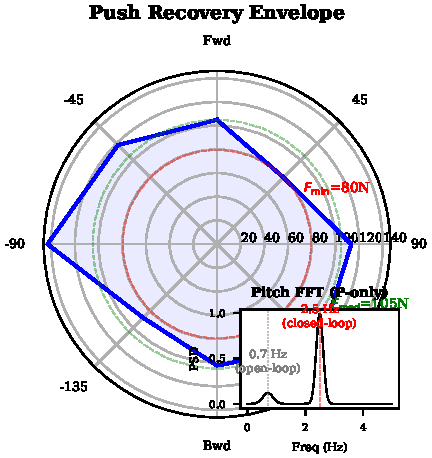
\includegraphics[width=\linewidth]{figures/polar_push_envelope.pdf}
    \caption{Omnidirectional push envelope of ACC. This is the \emph{same} run
    as row S1 of Table~\ref{tab:push_ablation}, not a separate measurement:
    \num{8} bearings, threshold located by
    binary search over \SIrange{10}{160}{N} to a \SI{5}{N} tolerance, so the
    plotted minimum is by construction the $F_{\min}$ of that row.
    $F_{\text{med}}$ is not read off this figure: it is the per-repetition
    median over the \num{8} bearings, averaged over repetitions
    (\SI{108.4}{N}), which differs from the median of the per-bearing means
    plotted here (\SI{105.6}{N}) because median and mean do not commute.
    Solid curve: per-bearing mean survivable push magnitude; shaded band:
    ${\pm}1$ standard deviation over the \num{30} repetitions. The radial axis is linear in force and
    originates at \SI{0}{N}, so radial distance is proportional to margin.
    The envelope is strongly anisotropic, spanning \SIrange{82.1}{144.1}{N}, a $1.8{\times}$ ratio between the weakest and
    strongest bearing. The ordering is
    $-\SI{90}{\degree}\,(\SI{144.1}{N}) >
      \SI{135}{\degree}\,(\SI{132.5}{N}) >
      \SI{90}{\degree}\,(\SI{115.8}{N}) >
      -\SI{45}{\degree}\,(\SI{110.5}{N}) >
      \SI{180}{\degree}\,(\SI{100.6}{N}) >
      \SI{0}{\degree}\,(\SI{95.5}{N}) >
      -\SI{135}{\degree}\,(\SI{91.8}{N}) >
      \SI{45}{\degree}\,(\SI{82.1}{N})$.
    Two regularities are visible. First, the actuated axis is the strong one:
    bearings are applied in the world frame as
    $\mathbf{f}=F(\cos\theta,\sin\theta,0)$, so $\pm\SI{90}{\degree}$ are purely
    sagittal and $\SI{0}{\degree}/\SI{180}{\degree}$ purely lateral
    (Section~\ref{sec:standing}). The two sagittal bearings average \SI{130.0}{N}
    against \SI{98.0}{N} for the two lateral ones, a $1.33{\times}$ advantage.
    This is the expected asymmetry for a wheeled biped: sagittally the wheels
    accelerate the contact patch back under the CoM and convert the impulse into
    a controlled excursion, whereas laterally no actuator produces ground force
    at all and the only restoring authority is the static
    $w_{\text{track}}={\SI{0.278}{m}}$ track width plus hip-roll PD. We compare
    axis \emph{means} rather than ranks because the raw ordering is contaminated
    by the second regularity. Second, the envelope is
    measurably \emph{chiral}: $\SI{135}{\degree}$ survives \SI{40.7}{N} more than
    $-\SI{135}{\degree}$, and $-\SI{90}{\degree}$ \SI{28.3}{N} more than
    $\SI{90}{\degree}$. This is not sampling noise and not the plant, which is
    mirror-symmetric to numerical precision: it is the sign convention of the
    controller's antisymmetric hip-roll and hip-yaw channels, which leaves the
    closed loop $C_2$-equivariant but mirror-broken. The
    text traces it through the $\sin2\theta$ harmonic and closes the argument
    with two control experiments. $F_{\min}$ (red) is the bearing-wise minimum
    and is the figure of merit quoted throughout the paper, because it is the
    magnitude survived in \emph{every} direction; $F_{\max}$ (blue) is shown
    only to indicate the spread.}
    \label{fig:push_polar}
\end{figure}

\begin{figure}[pos=!htbp]
    \centering
    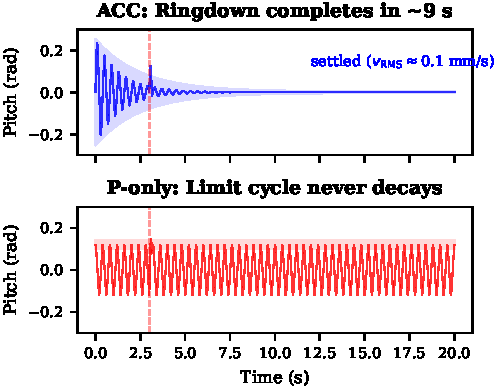
\includegraphics[width=\linewidth]{figures/ringdown_time_series.pdf}
    \caption{Post-push recovery (\SI{90}{N} lateral, world $+x$, at $t{=}\SI{3}{s}$). \textbf{Top:} attitude angles; stabilization within \SI{2}{s}. \textbf{Bottom:} planar CoM position, which separates the two axes cleanly. The lateral push couples through roll into a large \emph{sagittal} excursion (\SI{-251}{mm} peak); the anchor drives that axis back to $\SI{+1.37}{mm}$ of home and holds it there at \SI{0.018}{mm} SD over the final \SI{2}{s}, a \SI{99.5}{\percent} recovery. On the pushed lateral axis, which has no actuator authority (Section~\ref{sec:standing}), the \SI{200}{mm} peak excursion decays only to a permanent $\SI{+36.2}{mm}$ offset, \SI{18}{\percent} of the peak. The contrast between the two traces is the clearest single illustration of what the anchor does and where it does not act.}
    \label{fig:ringdown}
\end{figure}

\subsection{Flight Recovery and Terrain Adaptation}
\label{sec:flight_terrain_results}

ACC's two-channel assembly supports independent extensions without modifying the
core anchor, and both extensions use the same \SI{400}{Nm/s} rate limit and
\SI{100}{Hz} control rate.

Turning first to contact-loss recovery, ACC returns to a settled stand from a
\SI{100}{cm} free drop in \num{10} of \num{10} trials at $24.0{\pm}1.2^\circ$
peak pitch after touchdown, and from a \SI{50}{cm} ledge drive-off in \num{10} of
\num{10} at $27.1{\pm}2.0^\circ$, with the \SI{60}{cm} drop at
$18.2{\pm}1.0^\circ$ and the \SI{20}{cm} ledge at $19.6{\pm}0.3^\circ$
correspondingly milder.\footnote{All at \SI{400}{Nm/s} rate limit and
\SI{100}{Hz} control, $N{=}10$ per condition with randomized initial conditions
of $\pm\SI{0.003}{rad}$ per joint and $\pm\SI{1.5}{mm}$ on the CoM, $\pm$
denoting the standard deviation. Survival is the strict settle verdict, namely a
flat pitch and roll window, tail height error at most \SI{12}{mm} and residual
speed at most \SI{0.05}{m/s}, rather than merely staying upright; the drop metric
is peak $|\theta|$ from touchdown onward and the ledge metric peak $|\theta|$
through landing, while the curb metric is max $|\phi|$ while straddling, over
traversing trials only. Produced by
\path{scripts/collect_flight_terrain_n10.py}; raw output
\path{outputs/flight_terrain_n10/results.json}.} The two flight
ablations give a more nuanced picture than the mechanism's design rationale
suggests. Removing the flight attitude PD while retaining spin-down damping is a
real but modest loss, peak pitch rising to $27.8{\pm}0.3^\circ$ on the
\SI{100}{cm} drop with one fall in ten and to $31.6{\pm}2.2^\circ$ on the
\SI{50}{cm} ledge with none, whereas removing the airborne wheel-torque
override
entirely, so that the ordinary wheel--inverted-pendulum loop keeps driving the
wheels through flight, does not degrade either condition and in fact halves peak pitch to
$13.0{\pm}0.5^\circ$ and $10.2{\pm}0.4^\circ$ at full survival, because free
wheels driven by the pitch-feedback loop are themselves an effective reaction
flywheel. The override's benefit appears only at
the upper end of the envelope, where at \SI{150}{cm} the two configurations
survive equally at \num{2} of \num{5} but the override holds peak pitch to
$34.0{\pm}\SI{2.1}{\degree}$ against $53.6{\pm}\SI{35.0}{\degree}$, a sixteenfold
reduction in spread with one uncontrolled trial exceeding \SI{90}{\degree}, while
at \SI{200}{cm} both fail. The override therefore bounds landing-attitude
variance near the envelope limit rather than enabling the recovery, and at the
\SIrange{50}{100}{cm} scales reported here ACC's balance core alone suffices.

The success criterion for terrain adaptation is traversal rather than mere
survival, so a trial counts only if the elevated wheel stays on the
\SI{36}{cm}-wide slab for the whole \SI{2}{m} straddle. A settling criterion
alone cannot see this failure, because a robot that yaws off the side of the curb
halfway along still lands on flat ground, settles and would score a pass on the
tail criteria. Under the traversal criterion, and with the straddle gating of
Section~\ref{sec:terrain}, roll on the one-wheel curb at \SI{0.15}{m/s} measures
$2.4{\pm}\SI{0.1}{\degree}$ at \SI{10}{cm}, $2.9{\pm}\SI{0.2}{\degree}$ at
\SI{15}{cm} and $3.9{\pm}\SI{0.1}{\degree}$ at \SI{20}{cm}, with \num{10} of
\num{10} traversals at every height as Fig.~\ref{fig:curb} shows. The residual
growth with step height is tracking error rather than a geometry failure, since
mid-straddle at \SI{20}{cm} Eq.~\eqref{eq:terrain_split} commands a leg-length
difference of \SI{0.193}{m} against the \SI{0.20}{m} step, leaving
$\varepsilon{=}\SI{7}{mm}$ unspanned and hence a predicted
$\arctan(\varepsilon/w_{\text{track}}){=}\SI{1.4}{\degree}$ of geometric roll, so
the remaining \SI{2.5}{\degree} is servo error arising because in this deeply
flexed configuration the compressed leg carries its load at the shortest
gravitational moment arm the PID gains were tuned for. The joint budget tightens
with height without binding at \SI{20}{cm}, the compressed leg's commanded knee
angle growing from \SI{2.18}{rad} to \SI{2.58}{rad} against a \SI{2.70}{rad}
limit. With a split-independent roll band in the stability envelope, by contrast,
heading hold is suppressed through the straddle, the mount transient is left
undamped, the yaw error runs to the \SI{0.30}{rad} command leash and the elevated
wheel leaves the slab \SI{1.3}{m} into the curb, whose tight standard deviation
is a deterministic runaway rather than genuinely low run-to-run variability, the
measured roll being $14.9{\pm}\SI{0.1}{\degree}$ over ten trials with none
traversing.

The two component ablations are unambiguous. Replacing the split with a symmetric
posture that commands both legs to the same height causes a fall at every tested
curb height without exception, the torso rolling past \SI{60}{\degree} within
\SI{0.8}{s} of curb entry, so the height split is load-bearing for this task in a
way the flight override is not. Disabling the closed-loop leveling trim alone
leaves the robot upright and traversing on the \SI{10}{cm} curb at
$4.5{\pm}\SI{2.3}{\degree}$ but collapses the \SI{15}{cm} curb to \num{1} of
\num{10} and the \SI{20}{cm} curb to none of ten with five outright falls, because the feedforward height-to-leg-length table
alone does not span a step this large and the residual it leaves grows faster
than the straddle allowance can absorb.

Driving off a ledge whose edge crosses the path at an angle $\phi$ releases the
two wheels a stagger interval $w_{\text{track}}\tan\phi/v$ apart, and only within
that interval can the leg split absorb the step. Instrumenting a \SI{30}{\degree}
exit over a \SI{20}{cm} step at \SI{0.7}{m/s} shows the window closing in
\SI{0.18}{s}, the split having commanded \SI{25}{mm} of differential leg travel
against the \SI{200}{mm} step when the trailing wheel lost contact so that the
torso absorbed the remainder at \SI{-33.1}{\degree} of roll against the
$\arctan(0.20/w_{\text{track}}){=}\SI{35.7}{\degree}$ a wholly unspanned step
predicts. The legs were not at their travel limit when contact was lost, with
\SI{99}{mm} of calibrated range unused, so the proximate failure is a race rather
than a saturation, though relieving it would not rescue this case because
\SI{20}{cm} is itself unspannable at nominal stance and the $\pm\SI{6}{cm}$
leveling trim is unavailable throughout, its gate requiring both wheels loaded.
Failure is consequently not monotone in step height, two regimes separating
according to whether the leading wheel reaches the lower ground before the
trailing wheel releases, since free fall over the step takes $\sqrt{2h/g}$ and is
comparable to the stagger interval at these heights. A shallow step lands the
leading wheel while the trailing wheel still bears on the platform, forcing the
straddle the legs cannot span, whereas a deep step releases both wheels together
and is handled by the flight path of Section~\ref{sec:flight}, so widening the
straddle regime requires knee range rather than gains.

We calibrate the boundary over \num{192} trials spanning \num{12} heights from
\SI{12}{cm} to \SI{40}{cm}, eight independent initial conditions and two angles,
with \num{43} of \num{96} settling at \SI{30}{\degree} and \num{24} of \num{96}
at \SI{45}{\degree}. Both regimes are real and the dead band
between them is wide. At \SI{30}{\degree} the shallow window runs to \SI{15}{cm}
at full success, degrades through \SI{17}{cm} and \SI{20}{cm}, and closes
completely over \SIrange{22}{27}{cm}, after which the deep regime reopens from
\SI{30}{cm} and peaks at \SI{37}{cm}. At \SI{45}{\degree} the shallow window is
essentially gone, holding at \SI{12}{\percent} for the shallowest step and at
zero from \SI{15}{cm} to \SI{25}{cm}, and the deep regime opens later, at
\SI{27}{cm}. That the window shrinks with angle is what the stagger interval
$w_{\text{track}}\tan\phi/v$ predicts, and it shrinks by roughly the right
factor. Two features are worth stating as measured rather than smoothed, in that
neither regime reaches full success at depth, the deep-regime maximum being
\SI{75}{\percent}, and the \SI{45}{\degree} sequence has a reproducible empty
cell at \SI{32}{cm} sitting between \SI{50}{\percent} and \SI{62}{\percent}
neighbours that the two-regime account does not predict. The boundary is
therefore calibrated as a success-probability field over launch height rather
than as a single threshold.\footnote{\path{scripts/ramp_step_tests.py}
with \path{--seeds}; raw output \path{outputs/oblique_regime/diag30_fine.txt} and
\path{diag45_fine.txt}. Each seed perturbs the initial joint angles by
\SI{3}{mrad} and the root by \SI{1.5}{mm}, so the eight trials per cell sample
initial conditions on an otherwise deterministic course.}

The gate structure isolates each extension to its physical regime without
re-tuning the anchor, and both extensions cost three lines of controller code
each. Their measured necessity nevertheless differs sharply, since the per-leg
height split is required for the curb task at every tested height whereas the
flight override is a variance-bounding refinement that only pays at the top of
the drop envelope.

\begin{figure}[pos=!htbp]
    \centering
    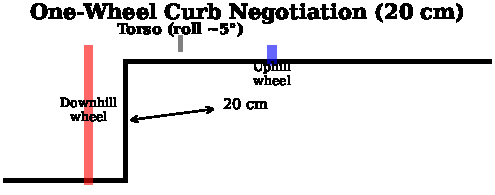
\includegraphics[width=\linewidth]{figures/curb_straddle.pdf}
    \caption{One-wheel curb (\SI{20}{cm}). With the per-leg height split and the
    straddle gating of Section~\ref{sec:terrain}: $3.9{\pm}0.1^\circ$ straddle roll,
    10/10 traversed. With a symmetric posture (split removed): the curb-side leg
    cannot fold far enough, roll diverges past \SI{60}{\degree} within
    \SI{0.8}{s} of curb entry, 0/10.}
    \label{fig:curb}
\end{figure}

\subsection{Comparison with Classical Baselines and a Preliminary RL Reference}
\label{sec:baselines}

No balance controller has been published for this morphology, a \num{10}-DOF
plant carrying three hip degrees of freedom per leg, so there is no established
classical design for it to compare against. Whleaper~\cite{whleaper2024} is the
closest published platform, and it switches between an LQR and a separately
trained policy by locomotion mode rather than closing every axis with one
controller. What can be measured in the absence of such a design is transfer,
meaning how far the reduced-order controllers the wheeled-biped literature does
publish carry when applied to this plant. The rows below should therefore be read
as a transfer result rather than as a ranking of ACC against optimal control, and
the row that tests the linear-design family on its own terms is the full-state
controller of Section~\ref{sec:full_state_lqr}, designed on a linearization of
this plant rather than of a simpler one.

Six classical baselines are evaluated alongside a preliminary model-free PPO run,
all sharing identical environment setups. Four are 4-state TWIP
variants~\cite{grasser2002joe,pathak2005wip}, namely a plain LQR with decoupled
roll and yaw PD through a PID servo layer of roughly \SI{0.25}{s} lag, the same
design augmented with a pitch-error integral under conditional anti-windup
clamped to $\pm\SI{3.0}{rad/s}$, a direct-torque LQR re-optimized for the
zero-lag plant, and a PI variant that adds integral anti-windup on forward
position behind a $\pm\SI{15}{cm}$ conditional gate. Two more are coupled 6-state
designs that extend the 4-state model with the roll states $(\phi,\dot\phi)$, one
acting through the servo layer and one emitting direct torques with gains
re-derived for the zero-lag plant and leg posture held by PD position control.
The seventh entry is a model-free policy trained from scratch for \num{5.4}M
environment steps in \texttt{BalanceEnv} on a single seed without domain
randomization or hyperparameter search, included as a difficulty probe rather
than as a tuned RL baseline in the sense of Limitation~4. Direct-torque LQR
removes the servo path and with it both the PID gains and the measured actuation
lag, while the PI variant adds the standard engineering fix for a DC position
bias together with windup protection, its anti-windup logic verified
independently by \texttt{scripts/validate\_lqr\_aw.py}. Every gain is listed in
the preceding paragraph, given in full because the central claim of this
subsection is a negative one, that no member of this family stands, and a
negative result is only as strong as the tuning behind it.

Every episode ends on roll. LQR balances wheeled bipeds on real hardware, as both
Ascento~\cite{klemm2019ascento} and DIABLO~\cite{diablo2024} demonstrate, and the
axis that terminates these episodes is not the one those platforms exercise. None
of these controllers fails at the task LQR is credited with there, since at
\SI{100}{Hz} the servo variants hold pitch to \SI{0.006}{\degree} RMS and the
full-state design of Section~\ref{sec:full_state_lqr} holds \SI{0.12}{\degree}
for the full \SI{20}{s}. What terminates every episode is roll, at
\SI{24.2}{\degree} RMS for the servo variants and \SI{21.2}{\degree} for direct
torque, on a morphology carrying two lateral degrees of freedom per leg that
those platforms do not have. The published designs do not ask a single LQR to
close that axis either, and DIABLO runs separate yaw, split-angle, height and
roll loops around its balance controller. Here the 4-state model carries no
lateral state at all, while the 6-state model carries roll but linearizes it
about one operating point and then commands the hip-roll channel against its
$\pm\SI{0.7}{rad}$ joint limit for the whole episode at every gain in an
eightyfold sweep. These rows therefore support a narrow morphological result,
that reduced-order LQR of the form the wheeled-biped literature uses does not
transfer to a 10-DOF articulated-leg plant as a single controller for all axes.
Whether LQR can balance a wheeled biped at all is settled elsewhere and in the
affirmative, and Section~\ref{sec:full_state_lqr} removes our tuning from the
statement by designing on the plant itself.

The same result appears inside ACC's own ablation ladder from the other
direction. Rung L0 is proportional-only on the wheel channel, carrying no
position term, no integral and no anchor, yet it stands in all ten trials where
an optimal law does not. L0 is not a linear controller for the whole robot but
ACC with the anchor removed, and it retains the dedicated roll, yaw and posture
channels that no row of Table~\ref{tab:lqr_baselines} has. The comparison in that
table is therefore neither optimal against hand-tuned nor linear against
nonlinear but one linearization for all axes against per-axis structure. Read
that way, the ladder and the baseline table state the same result from opposite
directions. Remove the structure and add optimality and the plant falls in
\SI{0.32}{s}, whereas keeping the structure and stripping everything else back to
a proportional term leaves it standing at \SI{17.461}{mm} repeatability inside a
\SI{69.7}{mm} limit cycle. That gap between L0 and ACC is what the remaining
terms buy, and it is measured in Section~\ref{sec:standing} rather than asserted
here.

Every baseline weight follows Bryson's rule~\cite{bryson1975optimal}, with
$Q_{ii}{=}1/x_{i,\max}^{2}$ and $R{=}1/u_{\max}^{2}$, and a
\num{46}-configuration retuning sweep confirmed that no retuning within these
ranges changes the outcome. The 4-state model carries pitch, pitch rate, forward
velocity and forward position and is solved at
$Q{=}\operatorname{diag}(10,2,3,0.3)$ with $R{=}0.8$, roll and yaw being closed
by decoupled PD through the PID servo layer, while the anti-windup variant adds a
pitch-error integral with conditional anti-windup clamped to
$\pm\SI{3.0}{rad/s}$. The 6-state model adds roll and roll rate and is derived in
continuous time at $Q{=}\operatorname{diag}(10,2,3,0.5,3,0.3)$ with
$R{=}\operatorname{diag}(0.8,1.0)$, shared by its servo and direct-torque
variants. Direct torque here means the PID servo path removed and the servo lag
$\tau_s$ set to zero, which requires re-optimization, giving
$k_{p,\text{roll}}{=}55.0$ in the 4-state case and $K_{\text{pitch}}{=}113$ with
$K_{\text{roll}}{=}\SI{58}{Nm/rad}$ in the 6-state case, and the PI variant adds
an integral on forward position at $k_{i,\text{pos}}{=}\SI{8.0}{rad/s/(m.s)}$
clamped to $\pm\SI{5.0}{rad/s}$ behind a $\pm\SI{15}{cm}$ conditional gate. The
servo layer itself runs $k_p{=}[55,40,70,70,4]$, $k_d{=}[3,2,4,4,0]$ and
$k_i{=}[0.8,0.4,1,1,0.1]$ ordered hip roll, hip yaw, hip pitch, knee and wheel,
and its lag of \SI{0.25}{s} is measured as the wheel-velocity \SI{90}{\percent}
rise time, roughly \num{25} steps at \SI{100}{Hz}.

\begin{table}[pos=!tbp]
\centering
\footnotesize
\caption{Classical baselines and the preliminary PPO reference vs.\ ACC, clean sensors. \textbf{Read the two attitude columns together:} every classical row is terminated by \emph{roll}, not pitch; $\theta_{\text{RMS}}$ stays between \SI{0.001}{\degree} and \SI{0.181}{\degree} while $\phi_{\text{RMS}}$ runs \SIrange{21}{28}{\degree}. None of these controllers fails at the sagittal task LQR is credited with on Ascento and DIABLO; they fail on a lateral axis their model does not carry. All rows at \SI{100}{Hz} control except the PPO reference, which is reported at the \SI{50}{Hz} rate its policy was trained at. Parenthesised $N$ is the episode count. See the note below the table.}
\label{tab:lqr_baselines}
\setlength{\tabcolsep}{4pt}
\begin{tabular}{@{}l S[table-format=2.2] S[table-format=1.3] S[table-format=2.2] S[table-format=3.1] S[table-format=2.2]@{}}
\toprule
Configuration & {Surv.} & {$\theta_{\text{RMS}}$} & {$\phi_{\text{RMS}}$} & {$H_{\text{RMS}}$} & {$\tau_{\text{RMS}}$} \\
& {(s)} & {(\si{\degree})} & {(\si{\degree})} & {(mm)} & {(Nm)} \\
\midrule
LQR, TWIP ($N{=}20$)         & 0.32 & 0.006 & 24.2 & 205.8 & 21.99 \\
LQR $+$ AW ($N{=}20$)        & 0.32 & 0.006 & 24.2 & 205.8 & 21.99 \\
LQR, DT (re-opt.) ($N{=}20$) & 0.60 & 0.033 & 27.5 & 119.2 & 8.76 \\
6-St.\ LQR ($N{=}20$)        & 0.32 & 0.006 & 24.2 & 205.8 & 21.99 \\
PI $+$ AW, DT ($N{=}20$)     & 0.52 & 0.181 & 26.1 & 171.3 & 10.42 \\
6-St.\ LQR, DT ($N{=}20$)    & 0.16 & 0.001 & 21.2 & 128.5 & 14.44 \\
PPO ref.\ (\SI{50}{Hz}) ($N{=}20$)& 3.20 & 4.82  & 3.15 & 54.2  & 18.40 \\
\addlinespace
\textbf{ACC} ($N{=}10$)      & \bfseries 20.00 & \bfseries 0.060 & \bfseries 0.010 & \bfseries 0.18 & \bfseries 3.28 \\
\bottomrule
\end{tabular}
\vspace{3pt}\tabnote\noindent\footnotesize
LQR / LQR+AW / 6-St.\ use the PID servo; LQR (DT), PI+AW (DT) and 6-St.\ (DT) command torque directly; PPO is a 5.4M-step single-seed run without domain randomization, a reference point rather than a tuned RL baseline. The three identical rows arise because all command through the same PID servo path, whose response dominates before their gain differential can act, a coincidence that holds at both control rates (Section~\ref{sec:rate_matched}).\tabnote\noindent
Between-episode standard deviations (omitted above for legibility): survival time is
deterministic on all six classical rows ($\pm\SI{0.00}{s}$ at $N{=}20$, seeds $\{0,42,123\}$);
PPO: $\pm0.85$, $\pm0.91$, $\pm0.45$, $\pm8.3$, $\pm2.1$;
ACC: $\pm0.00$, $\pm0.006$, $\pm0.001$, $\pm0.02$, $\pm0.00$.
Per-metric between-episode dispersions for the classical rows are not retained in the
rate-matched output (\path{outputs/rate_matched_baselines/results.json}), which stores
episode-aggregated values.
\vspace{2pt}\tabnote\noindent $N{=}20$ throughout; classical rows from \path{outputs/rate_matched_baselines/results.json}.
\end{table}

Table~\ref{tab:lqr_baselines} reports the comparison, and all six classical
baselines fall within \SI{0.60}{s}. Removing the PID servo path cuts torque by a
factor of \num{2.5} and nearly doubles survival from \SI{0.32}{s} to
\SI{0.60}{s}, yet it worsens roll from \SI{24.2}{\degree} to \SI{27.5}{\degree}
RMS, because the recovered authority is spent in the sagittal plane the model
describes rather than in the lateral one that ends the episode. Adding a
forward-position integral gives back \SI{0.08}{s} of that gain rather than adding
to it, since the integral cannot accumulate usefully before the roll-induced
fall, which confirms that the 4-state TWIP model is structurally insufficient for
this articulated-leg platform. The preliminary PPO reference sustains
single-height standing longer at \SI{3.20}{s} but exhibits an \SI{85}{\percent}
fall rate across multi-height command transitions with \SI{54.2}{mm} height
error, and that is the observation the structured prior is meant to address,
since unaided search spends its budget rediscovering the pitch--height coupling
that the posture map and the gate schedule encode directly. ACC by comparison achieves $0.060{\pm}0.006^\circ$ pitch RMS,
$0.010{\pm}0.001^\circ$ roll RMS, $0.18{\pm}0.02$\,mm CoM height RMS and
$3.28{\pm}0.00$\,Nm torque RMS over ten episodes, and the
\num{46}-configuration sweep along the dimensions of the preceding paragraph
found no exception anywhere among the tested variants.

\subsubsection{Both control rates give the same outcome}
\label{sec:rate_matched}

Table~\ref{tab:lqr_baselines} reports every classical baseline at ACC's
\SI{100}{Hz}, so the headline comparison carries no control-bandwidth
differential, but those gains were tuned for a \SI{50}{Hz} loop and all six were
therefore re-run at both rates. Doubling the control rate rescues none of them.
The fall rate is \SI{100}{\percent} in all twelve cells and survival time
improves for no variant, shortening for five of six. The diagnostic quantity is
roll, which sits at \SI{24.21}{\degree} at both rates for the three servo
variants and rises from \SI{21.22}{\degree} to \SI{27.48}{\degree} for the
direct-torque LQR, while faster sampling improves the quantities the controller
actually regulates, pitch RMS falling roughly sixfold for the servo variants and
torque RMS dropping from \SI{92.1}{Nm} to \SI{22.0}{Nm}. Leaving the lateral
divergence that terminates the episode untouched is the signature of a
model-structure deficit rather than of a bandwidth deficit, since the 4-state
TWIP model carries no lateral state at all and the 6-state variant linearizes
roll about a single operating point. Reporting the baselines at \SI{100}{Hz} is
thus the rate-matched choice and also the harsher of the two for them, since five
of the six survive longer at \SI{50}{Hz}.\footnote{$N{=}20$ episodes per cell,
seeds $\{0,42,123\}$, clean sensors, zero actuator delay, episode length fixed in
seconds rather than in steps. Produced by
\path{scripts/collect_rate_matched_baselines.py}, which adds a
\texttt{--control-hz} flag to \path{scripts/eval_balance.py}; raw output
\path{outputs/rate_matched_baselines/results.json}. The LQR feedback gains are
continuous-time and therefore rate-independent, so the rate change affects only
the substep count, the drift and integral accumulators, the torque rate limiter
and, for the finite-difference-linearized variant, the linearization step.}

\subsubsection{A full-state LQR designed on the plant itself}
\label{sec:full_state_lqr}

All six baselines above are designed on a reduced model, which confounds the
method with the model it is designed on. The control experiment that separates
the two is a linear-quadratic regulator derived from the plant directly. It
begins from a damped Gauss--Newton solve for a true static equilibrium
$(\mathbf{x}^\ast,\mathbf{u}^\ast)$ at the commanded height, takes central
differences on the whole held-input control step of the complete 16-DOF,
10-actuator MuJoCo model for the transition Jacobians, removes the two cyclic
wheel-angle states and closes with a discrete-time Riccati solve on the remaining
\num{30}. Torque is emitted under the same \SI{400}{Nm/s} rate limit as every
other row, and Bryson's rule~\cite{bryson1975optimal} fixes $\mathbf{Q}$ and
$\mathbf{R}$ from physical maximum deviations, leaving one knob, a uniform
control weight $r$, swept over six decades rather than tuned. The design is sound
on every diagnostic that bears on it, since at the \SI{0.65}{m} equilibrium the
residual unbalanced force is \SI{0.428}{N} against \SI{79.46}{N} of body weight,
the reduced $\mathbf{A}$ has full rank and is PBH-stabilizable, the Riccati
relative residual is of order $10^{-14}$ and the designed closed loop has
$\max|\lambda|{=}0.9911$. The one figure that invites a disqualifying reading,
$\kappa(\mathbf{A}){\approx}10^{10}$, does not support it, being a \SI{50}{Hz}
artifact that falls to $2.6{\times}10^{7}$ at \SI{100}{Hz} and tracing to a
smallest singular value of order $10^{-9}$ belonging to strongly contracting
contact modes. Whatever limits this controller, it is not the linearization.

What the sweep shows instead is a slow divergence that a short horizon hides.
Over \SI{20}{s} the design looks successful, $r{=}1000$ giving no falls at
$h{=}\SI{0.65}{m}$ with \SI{11.0}{mm} height RMSE, yet at \SI{60}{s} every
configuration tested falls in every episode between \SI{22.2}{s} and
\SI{57.0}{s}, with planar drift growing monotonically to
\SIrange{0.43}{0.63}{m}, and that drift rather than attitude is what ends them.
Nor does one weight cover the band, since $r{=}100$ stands \SI{20}{s} at
\SI{0.60}{m} and \SI{0.69}{m} but falls at \SI{0.65}{m} while $r{=}1000$ does the
reverse, under uniformly random height commands the fall rate runs
\SIrange{45}{80}{\percent} across the three usable weights, and at the baselines'
own \SI{50}{Hz} rate every weight falls inside \SI{20}{s}. Push separates it from
ACC outright, with total falls under the standard \SI{50}{N} impulse and a
maximum recoverable push of \SIrange{10.0}{20.2}{N} against ACC's \SI{82}{N}. The
reading is therefore not that the plant defeats linearization but that full-state
optimal linear feedback about a single equilibrium buys roughly two orders of
magnitude of survival over the reduced-order designs and still does not close the
problem, diverging slowly rather than quickly, holding one height at a time
rather than the band, and carrying essentially no push envelope. Two of those
three are exactly what the anchor integral and the gate schedule are for, which
is why the design is reported as a control experiment rather than promoted into
Table~\ref{tab:lqr_baselines}, since at the \SI{20}{s} horizon used for every
other row it would read as a partial success. That argument only carries if the
proposed controller is held to the same test, and it was, extending the
quiet-stance window by the same factors returning the opposite verdict for ACC,
which settles in every trial at \SI{300}{s} and \SI{1800}{s} with residual drift
of \SI{0.0004}{mm/min}.\footnote{$N{=}20$ episodes $\times$ seeds $\{0,42,123\}$ per configuration at \SI{100}{Hz}; between-episode SD is \SI{0.00}{s} on time-to-fall, and weights $r{<}100$ fall within \SI{1.4}{s}. Produced by \path{scripts/eval_balance.py --controller baseline_full_lqr}; per-configuration results and the design diagnostics are in \path{outputs/fullstate_lqr_corrected/}, whose \path{README.md} maps each row to its run.}

\subsubsection{Sensitivity of the coupled model's empirical roll coupling}
\label{sec:b_roll_hip}

The two 6-state coupled baselines close their roll channel with a constant
$b_{r,h}$ mapping hip-roll angle to roll acceleration that the planar pendulum
model does not supply in closed form, and it was set empirically to $-5.0$. Since
the negative result rests on those rows, that constant was swept over nine values
from \num{-0.5} to \num{-40} with gains re-derived through the same Riccati solve
at each value, and the outcome does not move, the servo variant falling at
\SI{0.320}{s} in every episode for every value and the direct-torque variant at
\SI{0.160}{s}, roll RMS staying constant to three decimals in both. This is
invariance to the parameter rather than insensitivity of the metric, because the
re-derived roll gain varies thirtytwofold across the sweep for the servo path.
The mechanism is saturation, since the roll-channel command reaches the
$\pm\SI{0.7}{rad}$ hip-roll joint limit at a roll excursion of
\SIrange{0.55}{17.87}{\degree} depending on $b_{r,h}$ while the excursion
observed before the fall has an RMS of \SI{24.2}{\degree}, so the channel is
commanded against its limit throughout the episode and the gain that computed the
command cannot matter.\footnote{Twenty episodes over three seeds at \SI{100}{Hz},
both variants; raw output \path{outputs/b_roll_hip_sweep/results_100hz.json},
produced by \path{scripts/sweep_b_roll_hip.py}.}

% ============================================================
\subsection{Whole-Body Control Baselines}
\label{sec:wbc}
% ============================================================

To address whether a tuned whole-body controller could match ACC we evaluated two
configurations developed and subsequently discarded during controller
development. The first is a task-priority quadratic-program WBC minimizing CoM
height error, torso orientation error, posture damping and wheel regularization
subject to full-body dynamics and contact constraints, used as the primary
balance controller. The second blends the same WBC as an assist on top of ACC
through $\boldsymbol{\tau}_{\text{assist}} = \boldsymbol{\tau}_{\text{ACC}} +
\alpha(\boldsymbol{\tau}_{\text{wbc}} - \boldsymbol{\tau}_{\text{ACC}})$ and is
evaluated both with the per-joint authority gate active and with it disabled.
Both run under identical cloned conditions as a three-arm counterfactual over
\num{225} scenarios spanning fixed-height balance, height transitions and push
recovery from \SI{20}{N} to \SI{120}{N}, totalling \num{481000} control steps
with no gain retuning, and so that the comparison is not a verdict on our own
implementation the WBC was verified beforehand against executable references as
Appendix~\ref{sec:wbc_supp} records.

Used as the primary controller, the standalone QP-WBC falls in all \num{225}
scenarios where ACC falls in none, holding the robot upright for \SI{0.570}{s}
and spending \SI{97.3}{\percent} of every episode in a fallen state. The failure
is lateral, roll RMS reaching \SI{93.45}{\degree} against ACC's
\SI{3.71}{\degree} and peaking past horizontal at \SI{103.9}{\degree} while pitch
RMS reaches only \SI{2.33}{\degree}, and base height collapses to \SI{0.091}{m}.
The fallen fraction is uniform across all five scenario suites, so the collapse
is specific to neither pushes nor commanded height changes.

The failure is invariant to implementation quality. A degraded build of the same
controller whose QP returns a usable solution on only \SI{85.85}{\percent} of
steps falls at \SI{0.52}{s} while the verified build, solving
\SI{99.99}{\percent} of steps, falls at \SI{0.570}{s}, so a fourteen-point
improvement in solve rate buys \SI{50}{ms} of upright time against a
\SI{0.570}{s} lifetime. Nor is it an artifact of one task weighting, since
re-running the WBC-only arm at four weightings over an identical scenario set
moves the fallen fraction by \num{0.1} percentage points and upright time by
\SI{0.03}{s}, the best mode improving pitch RMS by \SI{40}{\percent} at the cost
of roll because a single SO(3) orientation task carrying equal roll and pitch
gains trades one axis against the other rather than fixing both.

The mechanism is that the WBC's posture task is a velocity damper rather than a
position tracker. Its reference is rebuilt from the currently measured joint
vector at every control step, so the posture error vanishes identically and the
task collapses to $-k_{d,\text{posture}}\dot{\mathbf{q}}$ with
$k_{d,\text{posture}}{=}2.0$, which can slow a postural drift but cannot reverse
one. Combined with the absence of gravity-compensation feedforward, nothing in
the task stack restores the legs once a lateral excursion begins, which explains
why the collapse is lateral, why it is insensitive to the task weighting and why
solver quality does not delay it. The gap is one of structural expressiveness
rather than of torque optimality, because a WBC distributes torque optimally for
a fixed task set but cannot express quiet stance, push ringdown and large
excursion as distinct control modes, and the precision--recovery trade-off ACC
resolves through spatial gating and asymmetric envelope-following is not
expressible as a task-priority QP objective. Even an ideally implemented WBC
would therefore lack the prior that gates the anchor integral and would face the
global-integral windup that ablation S4 confirms is fatal for sub-millimetre
precision.

We ran the assist in both of its available configurations, which together
constitute the gate ablation reported in Table~\ref{tab:wbc_three_arm}. With the
gate disabled, so that $\alpha$ is fixed at \num{0.25} and per-joint authority is
capped at \SI{20}{\percent} of the ACC torque, WBC torque entered the blend
unconditionally. That arm never falls because ACC carries it, yet it degrades ACC
on every metric except one, raising pitch RMS
from \SI{0.520}{\degree} to \SI{1.295}{\degree}, yaw drift from
\SI{6.69}{\degree} to \SI{12.56}{\degree}, planar drift from \SI{0.099}{m} to
\SI{0.199}{m} and torque RMS from \SI{3.18}{Nm} to \SI{3.67}{Nm}. With the gate
enabled, so that per-joint authority becomes $\alpha_{j} =
\alpha_{\max}g_{\text{stability}}g_{\text{height}}g_{\text{push}}g_{\text{divergence}}A_jK_{\text{role},j}$,
instrumenting every factor at every control step shows the admitted authority
averaging \num{0.0061} on the one height variant where the gate opens at all,
some \SI{2.5}{\percent} of the permitted maximum, while on the remaining four the
height factor falls below its \num{1e-3} cutoff on the commanded height alone and
$\alpha$ is identically zero, so the gated assist is indistinguishable from ACC
alone to four significant figures. The two configurations therefore bracket the
assist, since where WBC authority is admitted it degrades ACC and
where it is harmless it is inactive, and no setting of the gate makes it
simultaneously active and beneficial.

Roll is the one metric WBC improves, and it is the exception in both
configurations, improving from ACC's \SI{3.71}{\degree} to \SI{3.20}{\degree}
over the full batch and from \SI{3.55}{\degree} to \SI{2.90}{\degree} on the
matched subset, which makes it systematic rather than sampling noise. ACC
regulates the lateral axis with decentralized hip-roll PD whereas the WBC uses a
centralized orientation task exploiting full mass-matrix coupling, so on that
axis alone the centralized formulation is the better regulator, but buying
\SI{18}{\percent} of roll costs two and a half times the pitch error and twice
the drift. A centralized lateral task is therefore a credible direction for
improving ACC's weakest axis, the \SI{98.0}{N} mean lateral push bearing of
Section~\ref{sec:push}, though not through torque-level blending with a posture
stack that cannot hold a posture. Timing is not what excludes it, since the QP
solve costs \SI{0.169}{ms} mean and \SI{0.30}{ms} at the 99th percentile over
\num{481000} solves with OSQP~\cite{stellato2020osqp}, comfortably inside the
\SI{10}{ms} control period, so the assist is excluded on control grounds alone.

\begin{table}[pos=!tbp]
\centering
\caption{Three-arm counterfactual under cloned initial conditions over \num{225} scenarios and \num{481000} control steps, comparing ACC alone, the standalone QP-WBC, and the WBC blended as an assist on ACC with its authority gate disabled. All arms use the verified WBC implementation of Appendix~\ref{sec:wbc_supp}.}
\label{tab:wbc_three_arm}
\footnotesize
\setlength{\tabcolsep}{3.5pt}
\begin{tabular}{@{}>{\raggedright\arraybackslash}p{0.34\columnwidth}rrr@{}}
\toprule
Metric & ACC & WBC & \multicolumn{1}{c@{}}{Assist} \\
\midrule
Scenarios with a fall      & 0/225 & 225/225 & 0/225 \\
Episode fallen (\si{\percent}) & 0.0  & 97.3   & 0.0   \\
Upright time (s)           & full  & 0.570   & full  \\
Pitch RMS (\si{\degree})   & 0.52  & 2.33    & 1.295 \\
Roll RMS (\si{\degree})    & 3.71  & 93.45   & \textbf{3.20} \\
Roll max (\si{\degree})    & 8.37  & 103.89  & 7.64  \\
Yaw drift (\si{\degree})   & 6.69  & 6.80    & 12.56 \\
Base height RMS (m)        & 0.540 & 0.126   & 0.518 \\
Final height (m)           & 0.538 & 0.091   & 0.515 \\
Planar drift (m)           & 0.099 & 0.165   & 0.199 \\
Torque RMS (Nm)            & 3.18  & 0.96    & 3.67  \\
QP success (\si{\percent}) & ---   & 99.99   & 100.00 \\
\bottomrule
\end{tabular}
\vspace{4pt}\tabnote\noindent\footnotesize
``Full'' upright time denotes no fall in any episode. Base height RMS is the root-mean-square of \emph{absolute} base-$z$, so a larger value means the robot stayed up and WBC's \SI{0.126}{m} is a collapsed torso rather than tighter tracking, just as its \SI{0.96}{Nm} is the torque of a machine lying on the ground. Roll is the sole metric on which the assist beats ACC (bold). The gated column is omitted because on the four height variants where its gate is identically closed it was not run, and on the fifth it agrees with the ACC column to four significant figures.
\end{table}



% ============================================================
\subsection{Architectural Analysis}
\label{sec:analysis}
% ============================================================

We evaluate ACC along four dimensions, namely robustness to noise and delay, gate
parameter sensitivity, torque rate-limit invariance and compound-disturbance
recovery. A factorial sweep over four noise levels and three delay levels, with
twenty trials in each of the twelve cells, bounds the first two axes at
once.\footnote{Noise at $1\sigma$: low is \SI{0.01}{rad/s} on angular velocity,
\SI{0.01}{m/s^2} on gravity and \SI{0.001}{rad} on joint position, medium is
$5\times$ and high is $10\times$ that. Delay is a transport lag on the actuator
command, the torque written $n$ control periods ago being the one the plant
receives. Idle RMS is the lateral CoM standard deviation over \SI{20}{s} after a
\SI{3}{s} settle from $\mathrm{EMA}_0{=}0$, averaged over surviving trials only,
so the medium-noise \SI{10}{ms} cell is mildly optimistic and its falls column is
the primary metric; $F_{\max}$ is a binary-search lateral push to
$\pm\SI{5}{N}$ with a \SI{10}{N} search floor. Produced by
\path{scripts/collect_robustness_sweep.py}, raw output
\path{outputs/paper_statistics/robustness_sweep.json}.} Measured cell by cell,
$F_{\max}$ is $95.7{\pm}\SI{0.8}{N}$ on clean sensing at zero delay,
$96.0{\pm}\SI{1.0}{N}$ under low noise and $93.5{\pm}\SI{5.2}{N}$ under medium,
falling to \SIrange{50.5}{51.3}{N} across all three at \SI{10}{ms}, while idle
lateral RMS runs \SI{0.43}{mm}, \SI{5.86}{mm} and \SI{30.82}{mm} undelayed and
\SI{2.43}{mm}, \SI{10.66}{mm} and \SI{35.38}{mm} at \SI{10}{ms}. One
control period of delay proves benign for stability and expensive for
performance, since at \SI{10}{ms} there are no falls on clean and low noise but
$F_{\max}$ bifurcates from \SI{95.7}{N} to \SI{50.5}{N} and idle RMS rises more
than fivefold. Three control periods is a different regime entirely, the platform
falling in every trial at \SI{30}{ms} on clean sensing and equally under low and
medium noise with no recoverable push at any tested magnitude, so delay tolerance
is bounded rather than open-ended and the bound lies between one and three
control periods, which the finer sweep below locates to \SIrange{14}{16}{ms}.
Noise alone is survivable up to the medium level at zero delay. What ACC does not
tolerate is the conjunction, since medium noise together with \SI{10}{ms} of
delay costs two falls in twenty trials, the only sub-catastrophic falls anywhere
in the grid, every other fall being a cell in which all twenty trials fail, while
high noise is unrecoverable at every delay including zero because the asymmetric
envelope cannot distinguish noise from motion, which forces anchor disengagement
and leaves a residual proportional mode that cannot hold the platform. That
conjunction is the binding constraint on the design, and
Section~\ref{sec:parking_supp} shows it is what prices the one gain change that
would otherwise remove ACC's parking offset.

That seventyfold idle degradation from clean sensing to medium noise at zero delay is
the sharpest single sensitivity in the design, produced by the same mechanism,
since the envelope gate cannot separate sensor noise from real motion and so
releases the integral and re-engages it repeatedly. That locates the boundary of
the anchored regime, because below it the anchor delivers the precision of
Table~\ref{tab:standing} whereas at medium noise it no longer pays for itself,
the un-anchored L0 baseline holding \SI{3.675}{mm} on the same axis. The design
requirement that follows is explicit and testable, namely that ACC is specified
against a filtered velocity estimate, which is a requirement on the state
estimator rather than a limit on the controller. One convention governs these figures, namely that the idle column is lateral
rather than sagittal and uses a \SI{3}{s} settling allowance, so its clean
reference is the \SI{0.43}{mm} entry and not ACC's lateral \SI{0.730}{mm}. Every
cell is measured identically and the degradation factors are the quantity the
sweep establishes.

The grid above quantises delay to the control period, so it brackets the useful
range at \SI{10}{ms} and \SI{30}{ms} without saying where inside that bracket the
behaviour changes. The knee was therefore located separately with the transport
delay applied per physics substep, which resolves the axis five times more finely
and is the more faithful model, since a real actuator's latency is not quantised
to the controller's period. Clean sensing makes the harness deterministic, every
multi-seed cell having returned identical values across seeds, so single-seed
cells are exact rather than sampled. That sweep places the knee between \SI{6}{ms}
and \SI{8}{ms}, $F_{\max}$ holding \SI{95.5}{N}, \SI{94.4}{N} and
\SI{93.2}{N} out to \SI{6}{ms} and then collapsing by \SI{45}{\percent} to
\SI{51.0}{N}, thereafter declining monotonically through \SI{41.6}{N} at
\SI{12}{ms} and \SI{28.8}{N} at \SI{16}{ms} to the search floor by
\SI{20}{ms}.\footnote{Transport delay applied per physics substep, \SI{2}{ms} at
\SI{500}{Hz}, which bounds the resolution and is why neither knee is localized
further; $F_{\max}$ by binary-search lateral push over seven iterations across
\SIrange{10}{160}{N}, clean sensing, $N$ up to \num{5}. The \SI{10}{ms} cell is
the only pure one-control-period hold, the others mixing two consecutive
commands within a period, which is why $F_{\max}$ is not smooth across it.
Produced by \path{scripts/delay_cliff_resolution.py} and
\path{scripts/delay_retune_sweep.py}; raw output in
\path{outputs/robustness_sweep/delay_cliff/} and \path{.../delay_retune/}.} That tail distinguishes a genuine loss of margin from a
narrow phase-alignment notch, and it is the former. The transition is a cliff
rather than a roll-off, so a design either clears it or does not, and the knee
sits below the \SI{10}{ms} figure the coarse grid implied while the end-to-end
budget estimated in Section~\ref{sec:discussion} lands inside the
\SIrange{6}{8}{ms} bracket rather than clear of it, which makes achieved latency
rather than architecture the deciding quantity. Absolute levels are not directly
comparable with the coarse grid, whose push protocol differs, but the
two harnesses agree on both anchors at \SI{95.5}{N} against \SI{95.7}{N}
undelayed and \SI{56.9}{N} against \SI{50.5}{N} at \SI{10}{ms}.

Losing the push margin and losing the platform are different thresholds, since
past \SI{8}{ms} the robot still stands and simply stops absorbing pushes. The
delay at which it stops standing at all was measured with the same substep
operator on a quiet-stance trial, and ACC holds station through \SI{14}{ms}
though visibly degraded, its idle lateral RMS running \SI{2.47}{mm} at
\SI{10}{ms} and \SI{10.84}{mm} at \SI{14}{ms} against \SI{0.43}{mm} undelayed,
falling at \SI{16}{ms} and beyond. The threshold is thus \SIrange{14}{16}{ms},
bracketed to one physics substep, and above it the collapse is prompt at
\SI{0.7}{s} for \SI{30}{ms}, which is what makes the \SI{30}{ms} column of the
coarse grid unanimous. One consequence bears on how the \SI{16}{ms} figure should
be read, because at that delay the quiet-stance trial diverges only at
\SI{22.0}{s}, later than the push harness's \SI{20.1}{s} horizon, so the
\SI{28.8}{N} recorded there is measured on a platform that is already unstable
and merely slow about it, and the last delay at which $F_{\max}$ describes a
platform that also survives the full quiet-stance window is \SI{14}{ms}.

Whether the knee belongs to the architecture or to the shipped gain set is a
question the sweep answers directly. Holding the delay at \SI{8}{ms} and sweeping
one profile constant at a time gives not a gently sloped optimum but a sharp
local dip, since the shipped value of each of the four constants tested scores
\SI{51.0}{N} while nearly every neighbouring value, in either direction and on
any of the four, recovers \SIrange{78}{93}{N}.\footnote{Velocity damping scale
swept over $\{0.5, 0.75, 1.0, \mathbf{1.5}, 2.0, 3.0\}$ for
\numlist{39.3;42.8;85.0;51.0;88.5;93.2}\,N; drift $k_{\text{vel}}$ over
$\{5,10,\mathbf{15},25,40\}$ for \numlist{65.1;92.0;51.0;90.9;80.3}\,N; soft
anchor $k_p$ pitch over $\{20,25,30,\mathbf{35},45,50\}$ for
\numlist{85.0;81.5;85.0;51.0;78.0;86.2}\,N; anchor $k_{\text{vel}}$ boost scale
over $\{0,2.5,\mathbf{5},10\}$ for \numlist{85.0;92.0;51.0;62.7}\,N. Shipped
values in bold, all other constants held at their promoted values, same push
protocol and bisection bracket as the resolution sweep, clean sensing and
$N{=}1$.} A margin that is genuinely exhausted does not behave that way, and the
shape is the signature of an unlucky phase alignment at one operating point,
which makes the \SIrange{6}{8}{ms} knee a tuning artefact rather than an
architectural ceiling.

Carrying the largest single-knob change forward, namely doubling the scheduled
sagittal damping from \SI{22.5}{} to \SI{45}{Nm/(m/s)} to give the variant we
denote ACC-DH, gives a controller identical to the shipped one at the shortest
delays, no worse at any delay tested, and with the knee moved outward by one grid
step to \SIrange{8}{10}{ms}, holding \SI{93.2}{N} at \SI{8}{ms} where the shipped
gains give \SI{51.0}{N} and adding \SIrange{44}{90}{\percent} of margin across
\SIrange{12}{16}{ms}, though both arms reach the search floor by \SI{20}{ms}, so
the retune buys headroom below the cliff without relocating the eventual failure.
The measured price is negligible at zero delay, undelayed idle lateral RMS rising
only from \SI{0.790}{mm} to \SI{0.801}{mm}, and real under delay, ACC-DH being
the less steady of the two at \SI{2.89}{mm} against \SI{2.47}{mm} at \SI{10}{ms}
while falling at the same \SI{16}{ms}, so the retune moves the push cliff without
moving the standing threshold. Under the noise-plus-delay conjunction it is
better rather than worse, its \SI{8}{ms} $F_{\max}$ rising from \SI{76.8}{N} to
\SI{92.0}{N} under low noise and from \SI{84.3}{N} to \SI{90.2}{N} under medium,
which also shows that the shipped controller's \SI{8}{ms} dip is deeper on clean
sensing than under noise and that the clean-sensing cliff is the conservative end
of the range. We report ACC-DH as an
evaluation variant and do not adopt it, since the constant it changes also
governs driving acceleration and settling and its cost on the driving, terrain
and flight axes has not been re-measured, a \num{48}-scenario qualification suite
rather than a single-axis sweep being what decides a default. The narrower claim
is sufficient for the limitation it addresses, that the delay knee is movable by
tuning at negligible cost to undelayed quiet stance, but that it buys push margin
only and leaves the
\SIrange{14}{16}{ms} standing threshold where it was.

Finite-difference gradients over the gate parameters reveal a stark hierarchy in
which the release coefficient $\alpha_r$ dominates at a sensitivity of
\num{220.4}, twenty times the next parameter and a hundred and thirty times the
pitch gates, whose near-zero sensitivity marks them as safety interlocks rather
than tuning knobs. Porting to a new morphology therefore starts by identifying
the dominant ringdown period from post-push decay and setting
$\tau_{\text{release}}$ to three to five times it, then setting the quiet-stance
band at two to three times the idle velocity noise floor and the pitch gates
conservatively at $\pm\SI{12}{\degree}$ and $\pm\SI{15}{\degree/s}$, a fixed
$k_p{=}50$ and anchor integral gain having sufficed here. The gate failure modes
themselves map onto measured ablation rows, which gives implicit FMEA coverage,
since a gate stuck open causes the windup and fall of S4, a gate stuck closed
yields the proportional-only limit cycle of L0, and a gate stuck half-open
triggers the parametric resonance of S5.

The \SI{400}{Nm/s} slew limit used throughout is not what sets ACC's push
ceiling. Sweeping it over an eightfold span, with each trial drawing an
independent initial-posture perturbation from the same distribution as the push
protocol of Section~\ref{sec:push}, gives lateral $F_{\max}$ of
$92.5{\pm}\SI{1.1}{N}$ at \SI{100}{Nm/s} and $94.4{\pm}\SI{0.0}{N}$ at
\SI{200}{}, \SI{400}{} and \SI{800}{Nm/s}, with idle lateral RMS between
\SI{0.695}{} and \SI{0.738}{mm} across the four settings, a \SI{2}{\percent}
spread in push margin and a statistically indistinguishable spread in idle
precision. The limiter is genuinely active where it could matter, since
instrumenting the commanded torque during a \SI{90}{N} push shows the slew
saturating exactly at each configured bound and even at \SI{800}{Nm/s} the wheel
channel still reaches it, whereas during quiet stance the peak commanded slew is
\SIrange{0.51}{1.66}{Nm/s}, some sixty to a hundred and ninety times below even
the \SI{100}{Nm/s} bound, so idle precision cannot be slew-limited at any tested
setting. The ceiling is therefore architectural rather than actuator-limited.%
\footnote{Sweep: \path{scripts/sweep_rate_limit_corrected.py}, raw output
\path{outputs/rate_limit_sweep/results_corrected.json}; slew instrumentation:
\path{scripts/probe_torque_slew.py}.}

The push protocol of Section~\ref{sec:push} holds the height command fixed, but
because the posture map is height-scheduled a commanded transition and a push
compete for the same leg-torque budget, so the two disturbances are evaluated
together here. The scenario applies the standard lateral push impulse at the
midpoint of a \SI{1}{s} commanded height ramp of size $\Delta h$ about the
\SI{0.404}{m} nominal CoM height and locates $F_{\max}$ by the same binary
search, with $\Delta h{=}0$ serving as the matched static control so that the two
differ only in the height command, ten trials to a row and each drawing an
independent initial posture. A commanded height change must move both the gain
schedule and the leg posture target, since ramping the schedule alone would leave
the robot standing at its nominal height with detuned gains, so both are ramped
and the achieved CoM height is verified against the model's own forward
kinematics before each sweep.\footnote{Binary search over
$[10,130]\,\si{N}$; rows within $\pm\SI{5}{cm}$ stay inside the calibrated
posture band \SIrange{0.354}{0.454}{m} while the $\pm\SI{10}{cm}$ rows are
extrapolated. Against the static control every row is significant under Welch's
$t$-test at the Bonferroni-adjusted $\alpha{=}0.0056$ of
Section~\ref{sec:discussion} except $-\SI{10}{cm}$ ($p{=}0.99$), and in the
re-calibrated arm only the $+\SI{10}{cm}$ row differs from the shipped map
($p{=}\num{1.5e-4}$), the other three lying within noise as they must, since the
two maps agree to \SI{3.2}{mm} inside the calibrated band. Peak pitch is measured
over the whole episode at each trial's own $F_{\max}$, so it is a shape statistic
at the survival boundary rather than a severity ranking across rows. Produced by
\path{scripts/compound_disturbance_corrected.py}; raw outputs
\path{outputs/compound_disturbance/results_corrected_map_shipped.json} and
\path{..._map_comcalib.json}, with posture-map accuracy verified by
\path{--self-check} against the model's own forward kinematics.}

Three findings follow. The first is that inside the calibrated posture band a
simultaneous height command is nearly free. Against the static control's
$94.8{\pm}\SI{0.8}{N}$, a ${+}\SI{5}{cm}$ rise costs \SI{5.1}{\percent} at
$89.9{\pm}\SI{0.9}{N}$ and a ${-}\SI{5}{cm}$ squat is better than static at
$101.0{\pm}\SI{1.0}{N}$, or $+\SI{6.5}{\percent}$, because squatting lowers the
CoM and shortens the toppling moment arm while the push arrives. Both effects are
statistically resolvable but operationally small, and since they bracket the
static value there is no shared-budget penalty at this amplitude.

The second finding is that the degradation is one-sided, so that descent is free
at any amplitude tested. Squatting ${-}\SI{10}{cm}$, fully outside the
calibrated band, costs nothing measurable at $94.8{\pm}\SI{1.9}{N}$ with
$p{=}0.99$, while rising ${+}\SI{10}{cm}$ falls to $29.7{\pm}\SI{8.7}{N}$, a
loss of \SI{68.7}{\percent}.
Extrapolation as such is therefore not the mechanism, direction is. Rising
drives the knee toward extension, where the leg Jacobian is worst conditioned
and the same joint torque produces the least vertical force, and it does so
while raising the CoM, whereas squatting moves in the opposite direction on both
counts and pays for it only in peak pitch, the $28.9{\pm}\SI{1.8}{\degree}$ of
the ${-}\SI{10}{cm}$ row being the largest measured, rather than in margin.
A control experiment separates how much of the remaining collapse is calibration
error and how much is the physics of standing tall. The shipped posture map is
exact inside its band but drifts outside it, undershooting the commanded CoM
height by \SI{10.0}{mm} at \SI{0.504}{m} and \SI{29.1}{mm} at \SI{0.554}{m}, and
re-parameterizing the same posture family so that the achieved height matches the
command, which changes no controller and is therefore only a relabelling, raises
$F_{\max}$ at ${+}\SI{10}{cm}$ by \SI{78}{\percent} to $52.8{\pm}\SI{12.1}{N}$
with $p{=}\num{1.5e-4}$ and drops the peak pitch from
$\SI{12.6}{\degree}{\pm}13.1$ to $\SI{8.8}{\degree}{\pm}2.3$. It does not restore
the static value, closing only \SI{35}{\percent} of the \SI{65.1}{N} deficit, so
the calibration error is a real and removable contributor but a minority one and
the residue is the genuine cost of carrying the load on a more extended leg.
Inside the band the two maps are indistinguishable, which is the control the arm
needs to be interpretable, and the large peak-pitch spread of the shipped
${+}\SI{10}{cm}$ row, with one trial reaching \SI{46.7}{\degree}, is consistent
with trials sitting on the edge of the capture basin, that spread rather than the
mean being what the re-calibration removes.

The third finding comes from a scenario that tests sequential rather than
simultaneous disturbance, a \SI{90}{N} lateral impulse followed \SI{2}{s} later
by a \SI{60}{N} counter-directed impulse delivered before the first ringdown has
fully decayed. ACC survives \textbf{10/10} with a Clopper--Pearson 95\% interval
of $[0.69,1.00]$ and an episode peak pitch of $11.89\pm\SI{0.51}{\degree}$,
essentially all of which comes from the first impulse, since after the reversal
the pitch peaks at only $2.78\pm\SI{0.11}{\degree}$ and never re-enters the
\SI{5}{\degree} band used as the settle criterion in any trial. The reversal is
thus absorbed within the residual motion of the first recovery, which is exactly
the behavior the asymmetric envelope is designed to produce, because
$\tau_{\text{release}}{\approx}\SI{1.5}{s}$ keeps the damping boost still partly
engaged when the second impulse arrives.

% ------------------------------------------------------------
\subsection{Local Stability Certificate at the Standing Fixed Point}
\label{sec:stability}

ACC's gates make it a switched system, which is why Section~\ref{sec:related_pos} places it alongside the switched-systems and hysteresis-switching literature~\cite{liberzon2003switching,hespanha2003hysteresis}. Everything reported so far is behavioral, in that the platform does not fall for \SI{30}{min} in Section~\ref{sec:longhorizon} and does not fall under any disturbance of Section~\ref{sec:push}, which is evidence rather than a stability statement. This section supplies one by locating the switching, characterizing the one live switch and examining the linearized closed loop.

At quiet stance the switching is inactive by a measured margin. Over the last \SI{20}{s} of a \SI{60}{s} settle, \num{19} of the \num{21} gates the controller exports sit at exactly \num{0} or exactly \num{1} at every control step, a bit-exact rather than an approximate saturation, while the two anchor gates that are not exported are reconstructed from controller state. The proximity gate's argument $|e_{\text{sag}}|$ peaks at \SI{24.8}{mm} against its \SI{50}{mm} knee, ranging over \SIrange{16.1}{33.2}{mm} across the five height variants for a margin of $1.5$--$3.1{\times}$, and the envelope gate's argument peaks at \SI{1.5e-7}{m/s} against its \SI{0.25}{m/s} knee, a margin of $1.7{\times}10^{6}$. Two gates do sit inside their bands, the anti-twist gate at ${\approx}\num{0.53}$ and the centering gate at ${\approx}\num{0.986}$, but a smoothstep is $C^\infty$ in the interior of its band, so those are ordinary smooth feedback rather than switching. In a neighborhood of the fixed point every branch selection in the controller is therefore frozen, the closed loop is a single smooth map, and Lyapunov's indirect method applies. Chattering is not avoided here because the gates are $C^1$, it is avoided because the operating point stands far from every switching surface, and the margins above are how far.

The one switch that does fire is a contraction on both branches. The asymmetric envelope of Eq.~\eqref{eq:asym_ema} selects $\alpha\in\{0.35,\,0.0067\}$ on the sign of $|v_{\text{sag}}|-\mathrm{EMA}_{t-1}$, and in quiet stance that sign flips at essentially every step, which is the composition flagged in Section~\ref{sec:overview} as only $C^0$ in time. For a fixed input level the tracking error $e_t=\mathrm{EMA}_t-|v_{\text{sag}}|$ obeys $e_{t+1}=(1-\alpha_t)e_t$, so $|e_{t+1}|\leq 0.9933\,|e_t|$ under either branch, making $V(e)=e^2$ a common Lyapunov function for the switched pair and the envelope globally exponentially stable under arbitrary switching at a worst-case rate set by the slow branch at $\tau{=}\SI{1.49}{s}$. The classical obstacle, that switching among individually stable subsystems can destabilize the whole~\cite{liberzon2003switching}, cannot arise, and no dwell-time or hysteresis condition is required~\cite{hespanha2003hysteresis}. The $C^0$ remark is thus discharged twice over, since the discontinuity lives in a provably contracting scalar subsystem and reaches the loop only through a gate that is flat at unity across the entire quiet band.

The linearized closed loop is obtained by central-differencing the whole \SI{100}{Hz} control step, meaning the control law together with its five physics substeps, about the settled state over an augmented vector of \num{57} coordinates. Of these, \num{30} are plant coordinates, namely \num{16} velocities and \num{14} configuration tangents once the two cyclic wheel angles are removed as in Section~\ref{sec:full_state_lqr}, \num{3} carry estimator memory and \num{24} carry controller memory. The adaptive-bias trim is held at its converged value because it is an \num{800}-tap moving average and therefore memory rather than dynamics, and freezing it makes the one-step map time-invariant instead of \num{300}-periodic. Table~\ref{tab:stability} reports that at all five heights the spectrum has exactly two eigenvalues on the unit circle, none outside it, and a reduced spectral radius of \numrange{0.99787}{0.99818}, corresponding to a slowest stable mode of \SIrange{4.7}{5.5}{s}. The classification is not a threshold judgement, because the gap from the unit circle down to the next mode is $1.8{\times}10^{-3}$, four orders of magnitude above the $10^{-7}$ sensitivity of the spectrum to the differencing step.

Both centre directions are identified and both are bounded by measurement. The first is lateral translation, which arises because a differential-drive base produces no lateral force to first order and appears at $|\lambda|{=}1$ to \num{e-12}, while the second is body yaw and is deliberate, since the heading channel carries an explicit deadband $\operatorname{ss}(|e_{\text{yaw}}|;\SI{0.02}{rad},\SI{0.08}{rad})$ measured at exactly \num{0} here, so absolute yaw enters no control law while the error stays inside $\pm\SI{1.15}{\degree}$. Neither is left to the linearization, since perturbing each coordinate and running \SI{300}{s} of the full nonlinear simulator returns a \SI{1.000}{mm} lateral offset to \SI{0.997}{mm} with no growth, while a \SI{0.500}{\degree} yaw offset creeps to \SI{0.565}{\degree} and would need \SI{3.3}{h} to reach the deadband edge at which heading control re-engages. The lateral mode is the same one the \SI{30}{min} run of Section~\ref{sec:longhorizon} measures as \SI{0.14}{mm/hour} of creep, so the certificate and the long run measure the same thing from two directions.

The linearization is finally checked against the plant it was taken from, random plant perturbations at \num{e-4}, \num{e-3} and \num{e-2} decaying in the full nonlinear simulator with nothing frozen at $\rho$ between \num{0.99513} and \num{0.99547} against the \num{0.99530} predicted for the anchor-integral mode at $\tau{=}\SI{2.12}{s}$, which is the mode a generic perturbation excites, so the agreement holds to \num{2e-4} over two decades of amplitude. What this does not establish is equally definite, in that the certificate is local, rests on the nominal model at zero delay and clean sensing, estimates no region of attraction, and excludes the push results of Section~\ref{sec:push} by construction, since a push is precisely what drives the gates off their flat regions and that is what the gates are for. What it does establish is that the point ACC parks at is exponentially attracting in \num{55} of \num{57} directions and neutral in the other two, with those two named, mechanistically explained and separately bounded.

\begin{table}[pos=t]
\centering
\caption{Local stability certificate at the standing fixed point, across the five calibrated height variants. Central-difference linearization of the \SI{100}{Hz} closed-loop step after a \SI{60}{s} settle; ``Flat'' counts exported gates that are bit-exactly saturated over the last \SI{20}{s}. $\rho_{\text{red}}$ excludes the two centre directions (lateral translation and deadbanded yaw), which are bounded separately by \SI{300}{s} nonlinear probes.}
\label{tab:stability}
\footnotesize
\setlength{\tabcolsep}{3.5pt}
\begin{tabular}{@{}lcccccc@{}}
\toprule
Height & CoM $z$ & Gates & Centre & Unst. & $\rho_{\text{red}}$ & $\tau_{\text{slow}}$ \\
variant & (m) & flat & dim. & & & (s) \\
\midrule
Nominal    & 0.4069 & 19/21 & 2 & 0 & 0.99818 & 5.49 \\
High small & 0.4164 & 18/21 & 2 & 0 & 0.99787 & 4.70 \\
High tiny  & 0.4128 & 19/21 & 2 & 0 & 0.99817 & 5.46 \\
Low small  & 0.3973 & 19/21 & 2 & 0 & 0.99813 & 5.34 \\
Low tiny   & 0.4009 & 19/21 & 2 & 0 & 0.99815 & 5.41 \\
\bottomrule
\end{tabular}
\tabnote{\sloppy Produced by \path{scripts/acc_stability_certificate.py}; full spectra, gate traces and probe trajectories in \path{outputs/paper_verification/} \path{acc_stability_certificate.json}. Spectra are insensitive to the differencing step at the $10^{-7}$ level.}
\end{table}

\subsection{Supplementary Video}
\label{sec:videos}

Thirty-one clips accompany this paper under \path{paper/videos/}, and they are
renders of the evaluation itself rather than a separate demonstration, since
\path{scripts/render_paper_videos.py} drives the same harness that produced the
corresponding table at the same seeds, so a clip and the number it illustrates
cannot drift apart. The inventory covers quiet stance, ten push trials spanning
the eight bearings of Fig.~\ref{fig:push_polar} together with one deliberate fall
at \SI{85}{N}, six drops from \SIrange{10}{100}{cm}, three curb straddles, eight
ledge courses and three commanded height transitions. Each clip is one trial at
one seed and therefore illustrates a regime rather than establishing a rate, the
rates being the $N{=}10$ and $N{=}30$ columns of the tables cited above, while
the noise and delay sweep, the classical-baseline comparison, the factorial
ablation and the parking-offset model are not filmed at all because they
distinguish their arms by numbers a viewer cannot see on a robot standing still.
The per-clip protocol and the measured outcome are given in
\path{paper/videos/README.md}.

% ============================================================
\section{Discussion and Conclusion}
\label{sec:discussion}
% ============================================================

ACC achieves all demonstrated behaviors without neural network training and is
hypothesized to carry a reduced sim-to-real transfer gap relative to learned
policies, pending hardware validation~\cite{grimminger2020torque}. Each gate was
added after tracing a measured failure mode to its root cause, those modes being
the bistable envelope, global-integral windup, parametric pumping, hard-leash
oscillation and self-referential stiffness, and all thresholds were frozen prior
to the ablation sweep of Table~\ref{tab:push_ablation}.

\subsection{Statistical Power}

All comparisons use Welch's $t$-test at a Bonferroni-adjusted
$\alpha{=}0.0056$ over nine comparisons. The push ablation is run at $N{=}30$,
where L0$\rightarrow$L1 and L2.5$\rightarrow$L3 are significant at
$p{<}\num{1e-15}$ with Cohen's $d$ of \num{4.3} and \num{3.6}, and the four
subtractive removals are bounded rather than merely non-significant, since
$|d|{\le}0.49$ and the shift on $F_{\min}$ stays below \SI{1.4}{N}. The primary
idle claims are stated as like-for-like ratios in Section~\ref{sec:standing},
namely $59.4{\times}$ sagittal, $22.6{\times}$ planar and $5.0{\times}$ lateral
repeatability, all of them L0 against ACC at $N{=}10$ under one protocol, with
the sagittal figure carried as the headline because that is the actuated axis.
The S5 collapse is unambiguous, at \num{0}/\num{10} survival when idle and
\num{10}/\num{10} at every push magnitude, and the flight and terrain rows are
$N{=}10$ with a Clopper--Pearson 95\% interval of $[0.69,1.00]$.

\subsection{Limitations}

The first limitation is that every result is obtained in simulation. All numbers
are MuJoCo, hardware validation remains future work, and the sim-to-real gap is
hypothesized to be reduced relative to learned policies rather than measured.

The second limitation, and the binding one for deployment, is timing. ACC as
tuned requires a \SI{100}{Hz} loop and an actuator latency clearing the \SIrange{6}{8}{ms}
push-margin cliff of Section~\ref{sec:analysis}, it stops standing by
\SIrange{14}{16}{ms}, and the \SIrange{6.6}{8}{ms} end-to-end budget estimated
below sits inside the cliff bracket, so a non-real-time build is not guaranteed
the nominal push envelope. Rate-independence is not claimed either, because at
\SI{50}{Hz} with coefficients recomputed for the longer step, giving
$\alpha_a{\approx}0.58$ and $\alpha_r{\approx}0.013$, the platform does not
stand at all and settles at a mean CoM height of \SI{0.124}{m} against the
\SI{0.404}{m} nominal. Whether that is excitation of plant modes the faster loop
suppresses or phase lag from discretizing the asymmetric envelope at
$\Delta t{=}\SI{20}{ms}$ is not resolved here and would require a loop-gain and
phase-margin analysis. Both thresholds are measured on clean sensing, and the
conjunction of noise with delay is bounded only by the \SI{10}{ms} and
\SI{30}{ms} columns of the noise--delay grid.

The third limitation is that two of the calibrated envelopes are non-uniform.
Oblique ledge descent has two survivable regimes separated by a dead band, as
the \num{192}-trial grid of Section~\ref{sec:flight_terrain_results} establishes, and since the
best cell reaches only \SI{75}{\percent} a clean launch is a favourable initial
condition rather than a guarantee, while the \SI{45}{\degree} course at
\SI{32}{cm} is a reproducible \num{0}/\num{8} that the two-regime account does
not predict. Upward height commands under simultaneous push are likewise
restricted, since a ${+}\SI{10}{cm}$ rise costs \SI{69}{\percent} of $F_{\max}$
while descent is free at every amplitude tested. A control experiment attributes
\SI{35}{\percent} of that deficit to posture-map parameterization and the
remainder to the physical cost of standing on a more extended leg, and the
re-parameterization is not shipped because changing the posture map would
require re-qualifying the standing suite against which it was frozen.

The fourth limitation is that the learning comparison is preliminary and one
classical family remains untested. The model-free PPO run of 5.4M steps used one
seed with no domain randomization~\cite{tobin2017domainrand,peng2018dynrand} and
no hyperparameter search, which makes it a difficulty probe whose
\SI{85}{\percent} fall rate bounds nothing about RL on this platform. The
comparison this controller is built for is residual learning over the prior
rather than against it, and that comparison is not run here, as
Section~\ref{sec:intro} states. Predictive control is the remaining untested
classical family, but which part of it a receding horizon would repair can be
identified rather than assumed. The full-state design of
Section~\ref{sec:full_state_lqr} fails in three separable ways, since it drifts,
it holds one commanded height at a time, and it has almost no push envelope, and
only the last two are open to a predictive formulation. A convex MPC over that
same linearization, with terminal cost set to the Riccati solution of that
design, emits exactly the LQR input at every step where no constraint is
active~\cite{rawlings2017mpc}, and across the entire pre-fall drift phase none
is active, because the configurations that fall at \SIrange{22}{57}{s} run at
\SIrange{2.0}{3.2}{Nm} torque RMS against a tightest actuator bound of
\SI{30}{Nm}, some \SIrange{7}{11}{\percent} of it, and under \SI{2}{\percent} of
the \SI{150}{Nm} hip-pitch and knee bounds. The drift is therefore not a horizon
artifact but a static offset that state feedback without integral action cannot
reject, and the predictive formulations that do reject it, meaning offset-free
MPC carrying an augmented disturbance state, reject it by adding integral
action, which is what the anchor is. What a receding horizon would genuinely buy
lies elsewhere, first in the push regime, where the torque bounds and the
$\pm\SI{0.7}{rad}$ hip-roll limit do bind and constraint-aware preview has no
counterpart among ACC's gates, and second across the height band, through
relinearization at each step rather than about a single equilibrium. Those two
are the comparisons left open, at a cost this paper can price, namely a dense QP
over \num{30} states and \num{10} inputs at \SI{100}{Hz} against the branchless
\num{27664}-flop control step priced below. The task-priority QP whole-body
controller of Section~\ref{sec:wbc} does not resolve the precision and recovery
trade-off, yet roll RMS is the single axis on which the blend beats ACC by
\SI{14}{\percent}, so the centralized formulation has merit that torque-level
blending cannot harvest. Push ablations at $N{=}30$ resolve about \SI{1}{N}, set
by between-episode dispersion rather than by the search bisection, and no claim
in this paper rests on a smaller difference.

The fifth limitation is that generality across morphologies is undemonstrated.
Every result is for one 10-DOF platform with one set of gains, and the porting
recipe of Section~\ref{sec:analysis} is a hypothesis derived from this
platform's sensitivity structure rather than a validated procedure.

\subsection{Deployment Risks and Mitigations}

ACC uses raw torque under a \SI{400}{Nm/s} rate limit with standard sensing from
an IMU and joint encoders. The binding latency figure is a performance cliff
between \SI{6}{ms} and \SI{8}{ms}, across which $F_{\max}$ falls from
\SI{95.5}{N} to \SI{51}{N} as Section~\ref{sec:analysis} shows, whereas below
\SI{6}{ms} the cost stays under \SI{2.4}{\percent}. The companion stability
threshold is roughly twice as far out, since on clean sensing ACC holds station
through \SI{14}{ms} and falls by \SI{16}{ms} as reported in
Section~\ref{sec:analysis}. That ordering is the one the architecture predicts,
because ACC's gates depend on physical state rather than on timing precision,
the proximity gate being spatial at \SI{15}{cm}, the asymmetric envelope being
temporal but slow at $\tau_r{\approx}\SI{1.5}{s}$, and the damping boost being
state-driven rather than schedule-driven. Twice is nevertheless a factor of two
rather than an order of magnitude, so a build that misses the latency target
does not merely lose push margin gracefully, and commissioning should be done
against the \SI{6}{ms} cliff rather than against the \SI{14}{ms} fall threshold.

The estimated worst-case budget for a non-RTOS build allows about \SI{1}{ms} for
sensor readout, about \SI{2}{ms} for state estimation, at most \SI{1.5}{ms} for
ACC computation and about \SI{3.5}{ms} for actuation latency, which totals
roughly \SI{8}{ms} end to end. Three of those four terms are assumed component
figures while the ACC term is measured, on the same footing as the QP solve time
reported for the discarded WBC baseline of Section~\ref{sec:wbc}. One control
step of the shipped profile costs \SIrange{1.11}{1.22}{ms} mean and
\SIrange{1.27}{1.52}{ms} p99 across five independent repeats of \num{5000}
consecutive steps taken at the quiet-stance operating point, of which the
compiled torque assembly itself accounts for \SI{0.05}{ms} mean and the
remaining \SI{1.15}{ms} is the CoM and support-polygon computation together with
Python-side dispatch. The \SI{1.5}{ms} carried into the budget is the rounded
upper end of that p99 range and it is doubly conservative, because the CoM
estimate inside it is part of what the separate \SI{2}{ms} state-estimation line
already accounts for and is therefore charged twice.\footnote{Produced by
\path{scripts/measure_control_step_cost.py}; raw output
\path{outputs/paper_verification/control_step_cost.json}, which is the last of
the five repeats. Host: Apple silicon (arm64), macOS, JAX CPU backend, Python
3.10.}

Wall-clock on a development host is nevertheless the wrong quantity to
extrapolate to an embedded target, and the reason is visible inside the
measurement, since five identical repeats give means spanning \SI{0.11}{ms}, p99
values spanning \SI{0.25}{ms}, and one worst single step of \SI{3.6}{ms} caused
by operating-system preemption rather than by anything the controller did. What
is reproducible instead is the operation count. XLA's cost model reports
\num{27664} floating-point operations and \num{159} transcendentals per control
step over a working set of \num{1001} scalars, identical to the last digit on
every repeat. The step contains no iterative solve, no matrix factorization and
no data-dependent control flow, every gate of Section~\ref{sec:anchor} being a
branchless select, so its worst-case execution time equals its average, which is
the property a hard real-time loop requires and which the QP-based alternative
cannot offer at all. At that count a \SI{480}{MHz} Cortex-M7 with a
single-precision FPU retires the step in about \SI{0.07}{ms} when charged one
cycle per operation and a conservative \num{40} cycles per transcendental, and a
\SI{100}{MHz} Cortex-M4 takes \SI{0.34}{ms}. Compute reaches the \SI{1.5}{ms}
budgeted above only on a part slower than about \SI{23}{MHz}, which is not a
processor anyone would put a \SI{100}{Hz} balance loop on. The compute term is
therefore the one entry in the budget that gets smaller on the deployment target
rather than larger, since roughly \SI{95}{\percent} of the measured
\SI{1.2}{ms} sits outside the compiled kernel, in the CoM and support-polygon
computation and the Python-side dispatch around it, work a C port either deletes
outright or reduces to a few hundred operations of forward kinematics. Charging
that line at an op-count-derived \SI{0.1}{ms} instead of the host figure puts
the end-to-end estimate at \SI{6.6}{ms}. Both ends are reported, \SI{8}{ms}
instrumented and \SI{6.6}{ms} projected, because the \SI{4.5}{ms} of sensor
readout and actuation between them is assumed in either case and is the larger
uncertainty.

Read against the cliff at \SIrange{6}{8}{ms}, the instrumented \SI{8}{ms} sits
at the top of the bracket and the projected \SI{6.6}{ms} at its bottom. Neither
clears it outright, and what decides the matter is not compute but the
\SI{4.5}{ms} of sensor readout and actuation latency, which are bus and actuator
properties rather than software. Two independent mitigations each move the loop
to the clearing side. On a real-time operating system with a dedicated
balance-loop microcontroller, whether \SI{1}{kHz} RT Linux or bare metal, jitter
is typically below \SI{0.1}{ms} and \SIrange{2}{4}{ms} of budget is recoverable,
which puts the loop at \SIrange{2.6}{4.6}{ms} on the projected figure and
\SIrange{4}{6}{ms} on the instrumented one, below the cliff at either end.
Separately, and without touching the schedule, doubling the scheduled sagittal
damping $s_v k_{\text{vel}}$ moves the knee out to \SIrange{8}{10}{ms}, which
the projected figure clears outright and the instrumented one reaches, at
negligible cost to undelayed quiet stance.
The two act on different quantities, one shortening the loop and the other
moving the cliff, so they compose rather than substitute. Real-time scheduling
remains the recommendation and the loop-latency target is \SI{6}{ms} end to end
rather than \SI{10}{ms}. The damping variant moves the push cliff only, leaving
the \SIrange{14}{16}{ms} fall threshold unchanged, so it widens the performance
margin without widening the safety one, and it is reported without being adopted
for the reasons given in Section~\ref{sec:analysis}, since re-qualifying it over
the \num{48}-scenario suite is the work a hardware build would justify. Neither
scenario has been validated on hardware, and latency characterization with an
oscilloscope and a jitter histogram is required before deployment, being the
measurement that decides which side of the cliff a given build lands on. The
discarded WBC-assist variant of Section~\ref{sec:wbc} is excluded from the
hardware path on control grounds rather than compute grounds, because its QP
solve costs \SI{0.169}{ms} mean and \SI{0.30}{ms} p99 over \num{481000} solves
and would fit the budget, yet admitting its torque degrades pitch by
$\num{2.5}\times$ and planar drift by $\num{2.0}\times$, while gating it to the
point of harmlessness also gates it to \SI{2.5}{\percent} of its permitted
authority. On hardware the \SI{0.294}{mm} sagittal repeatability is projected to
degrade to \SIrange{1}{3}{mm} once encoder quantization, backlash, stiction,
tire compliance and IMU noise are present, which is the same ordering the noise
columns of the noise--delay grid display, and commissioning should proceed
in stages from static torque to standing, then push recovery, then tethered
flight and finally terrain.

\subsection{Conclusion}

We presented ACC, a two-channel torque assembly in which a PD balance core is
augmented by a proximity-gated anchor integral, achieving $0.294{\pm}0.015$\,mm
idle repeatability on the sagittal actuated axis, a $59{\times}$ improvement
over the proportional-only baseline under one unified protocol at $N{=}10$ in
Table~\ref{tab:standing}, together with omnidirectional push survival at
$F_{\min}{=}\SI{82}{N}$ and $F_{\text{med}}{=}\SI{108}{N}$. Absolute accuracy on
that axis is reported separately and fully accounted for, since the robot parks
\SI{27.0}{mm} from the commanded home and holds that standoff to \SI{0.009}{mm}.
The closed-form model of Appendix~\ref{sec:parking_supp} predicts the offset as
the static price of a deliberately bounded integrator memory, matching the
measured torque balance to \SI{0.45}{\percent}, and both available corrections
are priced against the evaluation suite.

Six classical baselines, comprising four 4-state TWIP variants and two 6-state
coupled variants, all fail without exception, so adding integral action to
LQR-optimal feedback does not prevent the fall. Two control experiments test
that comparison rather than assume it. Sweeping the coupled model's one
empirical constant over an \num{80}$\times$ range moves the outcome not at all,
because the roll channel is saturated throughout, and a full-state LQR derived
from the plant itself, with a sound derivation, a \SI{0.54}{\percent}
equilibrium residual, a stabilizable pair and a control weight swept over six
decades, survives two orders of magnitude longer than the reduced-order designs
and still falls, holding one commanded height at a time and recovering at most
\SI{20}{N} of push.

ACC tolerates moderate noise, is insensitive to the actuator slew bound over an
$8{\times}$ span from \SI{100}{} to \SI{800}{Nm/s} with a \SI{2}{\percent}
spread in $F_{\max}$ and no resolvable change in lateral idle precision, and
handles contact loss and terrain without neural network training. Its sharpest
deployment constraint is actuator latency, since push margin collapses across a
cliff between \SI{6}{ms} and \SI{8}{ms} that the \SIrange{6.6}{8}{ms} budget
estimated for a non-real-time implementation lands inside rather than clear of,
so real-time scheduling, a delay-hardened retune, or both are what put a build
on the right side of it.

The contribution is thus a structured classical prior, an interpretable
controller whose gating encodes the plant's measured failure modes, offered as
such rather than as a competitor to a fully resourced learned policy. Everything
claimed for it is a directly measured property of the controller standing alone,
including the mechanism decomposition that assigns the precision to a specific
term, the chirality of the push envelope, the closed-form account of the parking
offset and the local stability certificate of Section~\ref{sec:stability}, so
the results do not wait on the residual stack the prior was built to serve. That
stack is one downstream use among the future work, alongside hardware
validation, EMA settle-time characterization, a properly resourced learning
comparison with multiple seeds, domain randomization and a tuned reward, and
extending conditional activation to locomotion.

% ============================================================
% REFERENCES
% ============================================================
% ============================================================
% ============================================================
\section*{Declaration of competing interest}
No potential conflict of interest was reported by the author(s).

\section*{Funding}
This research did not receive any specific grant from funding agencies in the
public, commercial, or not-for-profit sectors.

\section*{Declaration of generative AI and AI-assisted technologies in the writing process}
During the preparation of this work the authors used Anthropic Claude in order to
edit language and typeset the manuscript. All controller design decisions,
experimental protocols, numerical results, and scientific claims are the
authors' own. After using this tool the authors reviewed and edited the content
as needed and take full responsibility for the content of the publication.

\section*{Data availability}
% Zenodo version DOI for release v1.0.0. The concept DOI, which always resolves
% to the latest version, is 10.5281/zenodo.21861316.
The controller, the MuJoCo model, every evaluation script referenced above, and
the raw result files backing each table are publicly available at
\url{https://github.com/Thuong180702/Wheeled-bipedal-robot-simulation} at
release tag \texttt{v1.0.0}, archived at
\url{https://doi.org/10.5281/zenodo.21876576}. Each main results table names its producing
script and its raw result file in the note beneath it, and the remaining sweeps
are cited inline where they are discussed. The raw per-step records behind the
whole-body-control results of Section~\ref{sec:wbc} are collected under
\path{outputs/wbc_postfix_evidence/} and those behind
Appendix~\ref{sec:parking_supp} under \path{outputs/parking_offset_evidence/},
each directory's \path{README.md} mapping every file to the table it produces
and the latter also giving the worktree recipe for reproducing a gain arm
without disturbing the shipped profile. The \num{31} supplementary clips of
Section~\ref{sec:videos} are under \path{paper/videos/}, regenerated in full by
\path{scripts/render_paper_videos.py}; that directory's \path{README.md} gives
the per-clip protocol and the measured outcome each one illustrates.

\appendix
\section{Why Saturation-Triggered Anti-Windup Is Insufficient}
\label{sec:aw_supp}

Saturation-triggered anti-windup fires on actuator saturation, and on this
platform the position error grows to \SIrange{10}{30}{cm} during a push while
the wheels stay well within their \SI{20}{rad/s} range, so the trigger never
activates. A static dead-zone either over-restricts or under-restricts, whereas
ACC's proximity gate avoids both through a continuous smoothstep. State-gated
conditional integration is itself standard practice in process control, but ACC
couples spatial gating with asymmetric envelope-detected damping and so provides
a temporal gating that static-threshold schemes lack. The two anti-windup
augmented baselines are evaluated in Table~\ref{tab:lqr_baselines}, and a
broader comparison against the full anti-windup taxonomy is deferred.

% ============================================================
\section{WBC Baseline Implementation Details}
\label{sec:wbc_supp}
% ============================================================

\subsection{Provenance and Scope of the Claims}

Every WBC number in Section~\ref{sec:wbc} comes from a single campaign of the
verified implementation covering \num{225} scenarios and \num{481000} control
steps, whose full metric set is Table~\ref{tab:wbc_three_arm}, the
degraded-solver control experiment contributing only the \SI{85.85}{\percent} QP
success rate and the \SI{0.52}{s} time-to-fall taken from that build's comparison
report in \path{docs/validation/V3_vs_V3_Assist_comparison_report.md}. Exactly
one failure mechanism is asserted and it is verified directly in the source,
namely that the posture task is a velocity damper rather than a position tracker,
while two further mechanisms are excluded by the implementation itself. The QP is
not linearized at a fixed operating height, since the mass matrix, the bias
forces, the CoM Jacobian and the torso angular-velocity Jacobian are evaluated at
the current state on every control step and the module's only linearization is
the standard height-independent friction-cone pyramid, and the wheels are not
bare point contacts, since lateral no-slip and forward rolling constraints are
implemented and ran throughout the campaign. The architectural claim, that a
fixed-task-priority formulation carries no regime gating, therefore rests on the
invariance of the outcome to solver quality and task weighting rather than on any
deficiency specific to this implementation.

\subsection{WBC Task-Weight Ablation}

The standalone WBC's failure could in principle depend on the particular task
weighting adopted, so the WBC-only arm was re-run at four weightings over an
identical scenario set of \texttt{random\_push} at nominal height with seeds
201--205. The balanced default uses $w_{\text{torso}}{=}3$,
$w_{\text{com}}{=}3$ and $w_{\text{posture}}{=}1.5$, and each priority mode
raises its named weight to \num{10}. No weighting rescues the baseline. The
fallen fraction spans \SIrange{97.3}{97.4}{\percent} and upright time spans
\SIrange{0.56}{0.59}{s}, a spread of \num{0.1} percentage points and
\SI{0.03}{s}, against ACC's \SI{0}{\percent} fallen over the same scenarios.
Roll RMS runs \SIrange{92.86}{95.28}{\degree} and pitch RMS
\SIrange{1.52}{2.51}{\degree}, against ACC's \SI{3.71}{\degree} and
\SI{0.52}{\degree}. Torso priority gives the best pitch and simultaneously the
worst roll, because torso attitude is a single SO(3) task carrying equal roll
and pitch gains, so raising its weight redistributes error between the two axes
instead of reducing both. The four modes are
\texttt{balanced\_default}, \texttt{torso\_priority}, \texttt{posture\_priority}
and \texttt{com\_priority} in \path{wheeled_biped/wbc/offline_task_stack.py}.

\subsection{Assist Gate Decomposition}
\label{sec:wbc_gate_decomp}

The gated assist is inert because its authority gate is shut almost everywhere
on this scenario matrix. The height factor
$g_{\text{height}} = \exp[-((h-h_0)/\sigma_h)^2]$ uses $h_0{=}\SI{0.53}{m}$ and
$\sigma_h{=}\SI{0.025}{m}$ and is hard-zeroed below a \num{1e-3} cutoff, and
four of the five height variants command a base-$z$ far enough from $h_0$ that
the commanded-height term alone drives the gate shut before the measured height
is even considered, the factor running from \num{2.3e-34} at
\texttt{high\_small} through \num{2.4e-14}, \num{9.9e-11} and \num{1.1e-7} at
\texttt{low\_tiny}. Only \texttt{low\_small} at a commanded \SI{0.550}{m} leaves
it open, at \num{0.53}. Measured over \num{10775} control steps on that one
variant, the four state-dependent factors are \num{0.527} for height,
\num{0.876} for stability, \num{0.998} for push and \num{0.999} for divergence,
whose product is \num{0.461}, while the per-joint agreement term $A_j$ and role
weight $K_{\text{role},j}$ reduce the admitted authority by a further
\num{19}$\times$ to $\bar\alpha{=}\num{0.0061}$ with a maximum of \num{0.0146},
which is \SI{2.5}{\percent} of $\alpha_{\max}{=}0.25$. The remaining shortfall
between the factor product and the admitted authority is that the WBC's torque
opposes ACC's on most joints and disagreement attenuates the blend. Both $h_0$
and $\sigma_h$ are hand-tuned constants of ACC's own gate, $\sigma_h$ having
already been widened from \SI{0.015}{m}, so they bound the authority ACC grants
the WBC and are not a property of the WBC formulation, which is state-dependent
and carries no fixed validity band.

\subsection{Baseline Implementation Verification}
\label{sec:wbc_verification_sec}

A baseline reported to fail must be shown to be correctly implemented, or its
failure becomes evidence about the code rather than about the formulation. Four
properties on which a task-priority QP-WBC depends were therefore checked
against executable references before the campaign of Section~\ref{sec:wbc} was
run, and all four pass. The analytic contact-point translational Jacobian
matches MuJoCo's \texttt{mj\_jac} element-wise at both wheel contact points to a
maximum absolute error of \num{4.2e-8} over the full matrix and \num{3.4e-8}
over the actuated block, against an acceptance bound of \num{1e-3}, and the
ipsilateral leg columns are nonzero with norms
\numlist{0.042;0.433;0.403;0.306;0.060} while the contralateral columns are
exactly zero as the kinematics require, so there is no zero-gradient degeneracy.
The cached QP cost builder is parameterized by \texttt{task\_mode}, so the four
weightings above are genuinely distinct problems, the one call site passing a
literal being the task-independent constraint-only fallback that carries no cost
terms by construction. The batch runner reads the ACC height reference from the
scenario's \texttt{target\_com\_z} and no base-$z$ path into the height command
exists in the source, which matters because substituting one frame for the other
would inject a \SI{13.2}{cm} reference error under the convention of
Section~\ref{sec:height_convention}. Finally the adaptive-assist
$g_{\text{height}}$ gate is passed its own base-$z$ target rather than reusing
the CoM-$z$ reference, so gate and controller agree on the frame, and the gate
is nonetheless nearly shut on this scenario matrix for the tuning reason
quantified in Section~\ref{sec:wbc_gate_decomp}. The checks are executable
through \path{scripts/verify_wbc_audit_fixes.py} with archived output
\path{outputs/wbc_audit_fix_verification.json}.

Because gate and controller agree on the height frame, the gate's near-total
closure is a property of its tuning rather than of a frame mismatch, so the gated
assist's numerical equivalence to ACC follows directly from a gate that is shut
or nearly shut everywhere here and is not by itself evidence that the blend is
harmless. The evidence about the blend is instead the ungated configuration of
Section~\ref{sec:wbc}, which admits WBC torque on every step and degrades every
stability metric but roll.

% ============================================================
\section{Static Torque Balance of the Sagittal Parking Offset}
\label{sec:parking_supp}
% ============================================================

Section~\ref{sec:standing} reports a $\SI{-27.0}{mm}$ sagittal parking offset on
the axis the anchor integral regulates. This appendix derives the offset in
closed form from a measured torque decomposition, validates the derivation
against a $40{\times}$ gain sweep and a five-point height sweep, and reports the
measured cost of the available corrections. All runs use the idle protocol of
Table~\ref{tab:standing} with identical seeds, a \SI{5}{s} settle and a
\SI{20}{s} window, and the controller's internal sagittal torque decomposition
is logged alongside the gravity moment about the wheel axles by
\path{scripts/diagnose_parking_offset.py}, with raw records under
\path{outputs/parking_offset_evidence/}. Sagittal is world $y$ on this platform,
so the $x$ columns of the raw records are lateral.

\subsection{The offset is neither gravity-driven nor a saturated integral}

Two natural explanations fail on direct measurement, as Fig.~\ref{fig:parking}a
shows for $N{=}10$ with values averaged over the measurement window.

\begin{center}\footnotesize
\begin{tabular}{lr}
\hline
Gravity moment about the wheel axle & \SI{+0.0040}{Nm} \\
CoM lever arm about the axle & \SI{0.050}{mm} \\
Anchor integral $I$ & \SI{0.198}{Nm} (\SI{10.0}{\percent} of cap) \\
Integral clamp $I_{\max}$ & \SI{2.0}{Nm} \\
Pitch-loop torque $\tau_{\text{pitch}}$ & \SI{-1.2587}{Nm} \\
Position-loop torque $\tau_{\text{position}}$ & \SI{+1.2631}{Nm} \\
Adaptive bias trim $\tau_{\text{trim}}$ & \SI{+0.0655}{Nm} \\
Controller position error $e$ & \SI{-24.99}{mm} \\
Base parking offset $\bar{s}$ & \SI{-26.96}{mm} \\
\hline
\end{tabular}
\end{center}

Gravity is not the load. The moment is \SI{0.0040}{Nm} because the CoM sits
\SI{0.050}{mm} from the axle line, which is not a coincidence of tuning, since a
wheeled inverted pendulum that has stopped accelerating has necessarily brought
its contact patch under its CoM whatever its absolute position. The parking
offset is a displacement of the whole machine relative to the commanded home
rather than a static lean, so no relation of the form
$\tau_{\text{gravity}}(\bar{s})\approx\tau_{\text{integral}}$ can hold.

The integral is not saturated either. $I$ reaches \SI{10.0}{\percent} of its
clamp during quiet stance and never approaches it, so the offset is neither a
windup nor an anti-windup artifact and cannot be relieved by raising the clamp.
This is consistent with the ablation result of Table~\ref{tab:standing}, where
removing the proximity gate entirely in S4 reproduces ACC bit-for-bit. What does
balance is $\tau_{\text{pitch}}$ against $\tau_{\text{position}}$, to within
\SI{0.005}{Nm}.

\subsection{Origin of the constant pitch torque}

The sagittal pitch term is
$\tau_{\text{pitch}}=k_{p,\theta}(\theta-\theta_{\text{ref}})$ with
$k_{p,\theta}=\SI{50}{Nm/rad}$ at idle, and decomposing the commanded reference
at the nominal standing height $h{=}\SI{0.4040}{m}$ gives the following.

\begin{center}\footnotesize
\begin{tabular}{lr}
\hline
Feedforward equilibrium-pitch calibration & $+\SI{3.4963}{\degree}$ \\
Support-position outer loop (PD, $k_p{=}\SI{0.8145}{\degree/m}$) & $-\SI{0.0203}{\degree}$ \\
Low-band support term (gated off at this height) & $\phantom{+}\SI{0.0000}{\degree}$ \\
\hline
Commanded reference $\theta_{\text{ref}}$ & $+\SI{3.4760}{\degree}$ \\
Measured body pitch $\theta$ & $+\SI{2.0336}{\degree}$ \\
\hline
Residual $\theta-\theta_{\text{ref}}$ & $-\SI{1.4424}{\degree}$ \\
$\Rightarrow \tau_{\text{pitch}}$ & \SI{-1.2587}{Nm} \\
\hline
\end{tabular}
\end{center}

The decomposition closes to four decimal places, so the offset originates in a
\SI{1.44}{\degree} calibration error of the feedforward equilibrium-pitch map at
this operating point rather than in the anchor at all. The outer loop does
observe the \SI{25}{mm} error yet contributes only $\SI{0.02}{\degree}$ against
the $\SI{1.44}{\degree}$ it would need, because its integral channel is disabled
and it therefore has finite DC gain as well.

\subsection{Closed form}

The sagittal wheel torque during quiet stance is
$\tau_{\text{pitch}}+\tau_{\text{position}}$ with the position law unsaturated,
since $|\tau_{\text{position}}|\approx\SI{1.3}{Nm}$ against a \SI{4.0}{Nm} cap,
so that

\begin{equation}
\tau_{\text{position}} = -k_{pos}\,e + I + \tau_{\text{trim}}.
\label{eq:poslaw}
\end{equation}

The implemented anchor integral is leaky. Eq.~\eqref{eq:anchor} writes the ideal
integral for clarity, whereas the discrete update applied at every step is

\begin{equation}
I_{k+1} = (1-\lambda)\bigl(I_k - k_i\,\Delta t\,g_{\text{prox}}g_{\text{env}}\,e_k\bigr),
\label{eq:leaky}
\end{equation}

with $\lambda{=}\num{5e-3}$ per step as listed in Table~\ref{tab:parameters}. A
leaky integrator is a first-order lag rather than an integrator, so at a fixed
point with the gates open Eq.~\eqref{eq:leaky} gives $I^{*}=-k_{I,\text{dc}}\,e$
with

\begin{equation}
k_{I,\text{dc}} = k_i\,\Delta t\,\frac{1-\lambda}{\lambda}
= \num{4.0}\cdot\num{0.01}\cdot\frac{\num{0.995}}{\num{0.005}}
= \SI{7.96}{Nm/m},
\label{eq:kidc}
\end{equation}

which is one fifth of $k_{pos}{=}\SI{40}{Nm/m}$ rather than infinity.
Substituting into Eq.~\eqref{eq:poslaw} and imposing zero net sagittal torque
yields

\begin{align}
e_{ss} &= \frac{|\tau_{\text{pitch}}| - \tau_{\text{trim}}}
               {k_{pos} + k_i\,\Delta t\,(1-\lambda)/\lambda} \nonumber\\
       &= \frac{\num{1.2587}-\num{0.0655}}{\num{40}+\num{7.96}}
        = \SI{24.88}{mm},
\label{eq:parking}
\end{align}

against \SI{24.99}{mm} measured, an error of \SI{0.45}{\percent}. The
remaining \SI{2.0}{mm} between $e$ and the base offset $\bar{s}$ is accounted
for by the base-frame versus support-centre convention gap, so the two figures
are consistent once expressed in the same frame.

The conclusion is structural rather than incidental, in that no element of ACC's
sagittal position chain has infinite DC gain. The anchor integral is leaky by
design and the outer loop's integral channel is disabled, so a constant
disturbance torque must be paid for with a constant position error, and the
\SI{27}{mm} is the price of that design choice expressed in millimetres per
newton-metre.

\begin{figure}[pos=!htbp]
    \centering
    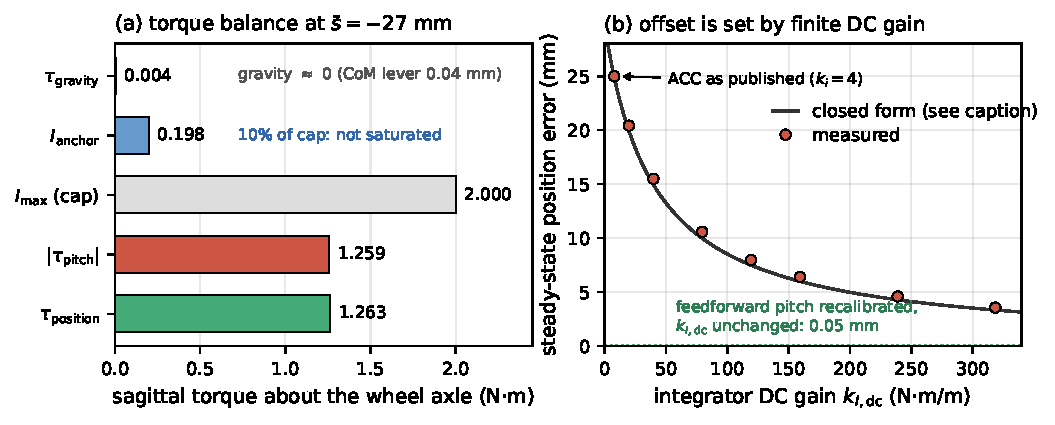
\includegraphics[width=\linewidth]{figures/parking_offset.pdf}
    \caption{Static torque balance of the sagittal parking offset.
    (a) Measured sagittal torques at the $\bar{s}{=}\SI{-27}{mm}$ parking point.
    The gravity moment about the wheel axle is \SI{0.0040}{Nm} and the anchor
    integral sits at \SI{10}{\percent} of its clamp, so the offset is neither
    gravity-driven nor a saturation artifact; the balance is between the
    pitch and position loops.
    (b) Steady-state position error against integrator DC gain
    $k_{I,\text{dc}}$ of Eq.~\eqref{eq:kidc}, swept over $k_i\in[4,160]$ at
    fixed leak. The curve is Eq.~\eqref{eq:parking} evaluated with the
    baseline $\tau_{\text{pitch}}$; using each run's own measured
    $\tau_{\text{pitch}}$ the closed form tracks all twelve gain and height
    points to within \SI{0.92}{\percent}. The dotted line is the same
    controller with the feedforward pitch reference recalibrated and
    $k_{I,\text{dc}}$ left unchanged.}
    \label{fig:parking}
\end{figure}

\subsection{Validation across a forty-fold gain sweep}

Sweeping $k_i$ from \num{4} to \num{160} at fixed leak moves $k_{I,\text{dc}}$
over $40{\times}$, and the offset follows Eq.~\eqref{eq:parking} throughout as
Fig.~\ref{fig:parking}b shows.

\begin{center}\footnotesize
\begin{tabular}{rrrrr}
\hline
$k_i$ & $k_{I,\text{dc}}$ & $e$ meas. & $e$ pred. & window jitter \\
 & (Nm/m) & (mm) & (mm) & (mm) \\
\hline
\textbf{4} & \textbf{7.96} & \textbf{-24.99} & \textbf{-24.87} & \textbf{0.298} \\
10 & 19.90 & -20.42 & -20.34 & 0.302 \\
20 & 39.80 & -15.49 & -15.54 & 0.147 \\
40 & 79.60 & -10.57 & -10.67 & 0.208 \\
60 & 119.40 & -7.96 & -8.01 & 0.168 \\
80 & 159.20 & -6.40 & -6.41 & 0.094 \\
120 & 238.80 & -4.59 & -4.58 & 0.114 \\
160 & 318.40 & -3.56 & -3.56 & 0.066 \\
\hline
\end{tabular}
\end{center}

Steadiness improves monotonically with $k_i$ over this range rather than
degrading, the opposite of the trade-off measured at $k_i{=}0$ in
Table~\ref{tab:standing}, which indicates that the $3{\times}$ steadiness cost
reported there is paid at the first newton-metre of integral authority rather
than progressively. Every entry is measured on clean sensing with no actuator
delay, which Section~\ref{sec:parking_ki_cost} shows is exactly the condition
under which raising $k_i$ looks free.

\subsection{Why the gain is not raised: the noise--delay cost}
\label{sec:parking_ki_cost}

The sweep above and the push protocol below both make $k_i{=}160$ look free,
since the offset falls by \SI{79.5}{\percent}, clean-idle jitter improves, and
neither $F_{\min}$ nor $F_{\text{med}}$ moves. Those three probes share a blind
spot, in that all are run on clean sensing and the push probe is a large
transient rather than a sustained small one. Re-running the two cells of
the noise--delay grid that combine medium sensor noise with actuator delay,
at $N{=}20$ per cell and identical seeds across arms, prices the change.

\begin{center}\footnotesize
\begin{tabular}{rrrrrl}
\hline
$k_i$ & $k_{I,\text{dc}}$ & $\bar{s}$ & offset & falls & Fisher \\
 & (Nm/m) & (mm) & removed & (of 40) & vs.\ $k_i{=}4$ \\
\hline
\textbf{4} & \textbf{7.96} & \textbf{-26.96} & \textbf{---} & \textbf{7} & \textbf{---} \\
20 & 39.80 & -17.47 & \SI{35.2}{\percent} & 13 & $p{=}0.196$ \\
40 & 79.60 & -12.55 & \SI{53.5}{\percent} & 10 & $p{=}0.586$ \\
80 & 159.20 & -8.37 & \SI{68.9}{\percent} & 14 & $p{=}0.126$ \\
160 & 318.40 & -5.53 & \SI{79.5}{\percent} & 17 & $p{=}0.027$ \\
\hline
\end{tabular}
\end{center}

A Cochran--Armitage trend test on $\log_2 k_i$ gives $z{=}2.34$ at $p{=}0.019$,
so the fall rate rises with integral gain across the sweep, and pooling every
arm above the shipped setting gives \num{54} falls in \num{160} against \num{7}
in \num{40} at $p{=}0.055$. Because the cost is graded rather than a threshold,
selecting the largest gain that is not individually significant would be an
artifact of sample size, since $k_i{=}40$ carries $p{=}0.59$ only because
\num{40} trials cannot separate \SI{17.5}{\percent} from \SI{25}{\percent}.
Zero-delay cells stay clean at every gain and the idle, push, flight, terrain
and rate-limit metrics are flat across the sweep, so the regression is specific
to noise and delay acting together. One trap is worth naming, namely that the
idle column of that grid averages survivors only, so in these
two cells the higher-gain arms report better idle numbers while falling more
often.

The mechanism follows from Eq.~\eqref{eq:leaky}. The leaky integrator has
transfer function $k_i\Delta t/(\lambda + s\Delta t)$, giving a DC gain of
$k_i\Delta t/\lambda$ and a corner at $\lambda/\Delta t\approx\SI{0.5}{rad/s}$.
Raising $k_i$ scales the response at every frequency, so it lifts mid-band gain,
carrying the \SI{90}{\degree} lag of an integrator, in precisely the band where
the \SI{10}{ms} actuator delay of those cells has already consumed the phase
margin. Lowering $\lambda$ raises DC gain alone and leaves mid-band untouched
but costs the memory horizon instead, as the next subsection shows. Neither
single parameter separates the two roles, and doing so would require a
lead-compensated or explicitly bandwidth-limited integrator, which is a
structural change to a controller whose present form is qualified over a
\num{48}-scenario suite and is therefore left as future work.

\subsection{The leak sets memory, not accuracy}

Because $k_{I,\text{dc}}$ depends on both $k_i$ and $\lambda$, reducing the leak
also raises DC gain, but it is the wrong knob. Cutting $\lambda$ from \num{5e-3}
to \num{5e-4} raises $k_{I,\text{dc}}$ to \SI{79.96}{Nm/m} and does reduce the
offset to \SI{-16.31}{mm}, yet window jitter degrades twelvefold from
\SI{0.298}{mm} to \SI{3.463}{mm} and the measured error of \SI{-14.34}{mm} does
not reach its DC prediction of \SI{-10.41}{mm}, because the forgetting time
constant $\tau{=}\Delta t/\lambda$ has grown to \SI{20}{s} and no longer settles
inside the measurement window. Since $\tau$ is independent of $k_i$ the two
parameters separate cleanly, $k_i$ setting DC gain and $\lambda$ the memory
horizon, and the shipped pair is chosen on that basis, $\lambda{=}\num{5e-3}$
fixing the \SI{2}{s} forgetting time that keeps the integral inside its
measurement window while $k_i{=}\num{4}$ is set not for clean-idle steadiness,
which the sweep shows is flat in $k_i$, but for margin against the conjunction of
noise and delay quantified in Section~\ref{sec:parking_ki_cost}. The accuracy
consequence of that pair is the \SI{27}{mm} offset, the price of the memory
horizon rather than of the gain.

\subsection{Two measured corrections and their cost}

The height dependence of the calibration error was checked on the five
posture-calibrated height variants by applying the correction measured at each
point. The nominal row is $N{=}10$ under the full idle protocol while the four
off-nominal heights are single trials, whose run-to-run spread the nominal row
bounds at \SI{0.011}{mm} SD.

\begin{center}\footnotesize
\begin{tabular}{rrrrr}
\hline
$h$ (m) & correction & $\bar{s}$ before & $\bar{s}$ after & reduction \\
 & (\SI{}{\degree}) & (mm) & (mm) & \\
\hline
0.394 & $-1.622$ & $-28.77$ & $-1.16$ & \SI{96.0}{\percent} \\
0.399 & $-1.974$ & $-34.53$ & $-1.20$ & \SI{96.5}{\percent} \\
\textbf{0.404} & $\mathbf{-1.461}$ & $\mathbf{-26.96}$ & $\mathbf{-2.02}$ & \textbf{\SI{92.5}{\percent}} \\
0.409 & $-0.943$ & $-19.29$ & $-2.83$ & \SI{85.3}{\percent} \\
0.414 & $-1.295$ & $-25.11$ & $-2.92$ & \SI{88.4}{\percent} \\
\hline
\end{tabular}
\end{center}

The controller's own position error falls to ${\leq}\SI{0.12}{mm}$ at every
height and the anchor integral to \SI{0.4}{\percent} of its clamp, so what
remains is the \SIrange{1}{3}{mm} frame-convention gap. The required correction
is not a constant, since it spans \SIrange{0.94}{1.97}{\degree} over
\SI{2}{cm}, which makes this a per-height recalibration of the feedforward map
rather than a single scalar.

Both corrections were then put through the full push protocol of
Section~\ref{sec:push}, meaning $N{=}10$ repetitions at each of eight bearings
with a binary search over \SIrange{10}{160}{N} at \SI{5}{N} tolerance and
Welch's $t$ against the published arm.

\begin{center}\footnotesize\setlength{\tabcolsep}{4pt}
\begin{tabular}{lrr}
\hline
Arm & $F_{\min}$ (N) & $F_{\text{med}}$ (N) \\
\hline
ACC as published ($k_i{=}4$) & 82.8(10) & 116.8(47) \\
$k_i{=}40$ & 81.8(18)\,\,$p{=}0.14$ & 116.8(70)\,\,$p{=}0.98$ \\
$k_i{=}160$ & 81.9(27)\,\,$p{=}0.32$ & 115.3(36)\,\,$p{=}0.43$ \\
Feedforward pitch recalibrated & 82.5(12)\,\,$p{=}0.55$ & 112.4(49)\,\,$p{=}0.05$ \\
\hline
\end{tabular}
\end{center}

The published arm reproduces the weakest bearing of Section~\ref{sec:push} at
\SI{82.8}{N} here against \SI{82.1}{N} there, a difference below \SI{1}{N} on
independent seeds, which validates the harness. Raising $k_i$ by $40{\times}$
costs nothing measurable on either push statistic and removes
\SI{79.5}{\percent} of the offset, while the feedforward recalibration removes
\SI{92.5}{\percent} and leaves $F_{\min}$ unchanged but shows a \SI{4.5}{N}
reduction in $F_{\text{med}}$, or \SI{3.8}{\percent}, at $p{=}0.051$, which at
this sample size is reported as unresolved rather than as null.

Neither correction is promoted into the shipped profile, and in the $k_i$ case
the reason is not consistency of the evidence base but a measured regression,
because the push protocol is blind to the failure mode that the gain change
introduces and that mode appears only when sustained sensor noise and actuator
delay act together, as Section~\ref{sec:parking_ki_cost} establishes. This is
the substantive result of the appendix. The \SI{27}{mm} offset is the position
error that a deliberately leaky and deliberately low-gain integrator pays in
exchange for a \SI{2}{s} forgetting horizon and for phase margin against delay.
Both alternatives were measured across the full evaluation suite rather than on
the accuracy metric alone, which is what exposed the price. The feedforward
recalibration remains the more promising route since its cost is confined to one
borderline statistic, and resolving that at a larger sample, together with
testing whether a bandwidth-limited integrator can raise DC gain without raising
mid-band gain, are the two concrete steps toward closing this limitation.

\begin{thebibliography}{99}
\setlength{\itemsep}{0pt}
\setlength{\parsep}{0pt}
\setlength{\topsep}{0pt}

\bibitem{klemm2019ascento}
V.~Klemm, et al., Ascento: a two-wheeled jumping robot, in: Proc. IEEE Int.
Conf. Robot. Autom. (ICRA), 2019, pp. 7515--7521.

\bibitem{klemm2020lqrwbc}
V.~Klemm, A.~Morra, L.~Gulich, et al., LQR-assisted whole-body control of a
wheeled bipedal robot with kinematic loops, IEEE Robot. Autom. Lett. 5 (2)
(2020) 3745--3752.

\bibitem{skater2024}
Y.~Wang, T.~Chen, X.~Rong, G.~Zhang, Y.~Li, Y.~Xin, Design and control of
SKATER: a wheeled-bipedal robot with high-speed turning robustness and terrain
adaptability, IEEE/ASME Trans. Mechatron. 30 (2) (2025) 1310--1321.

\bibitem{hwangbo2019rl}
J.~Hwangbo, J.~Lee, A.~Dosovitskiy, D.~Bellicoso, V.~Tsounis, V.~Koltun,
M.~Hutter, Learning agile and dynamic motor skills for legged robots, Sci.
Robot. 4 (26) (2019) eaau5872.

\bibitem{schulman2017ppo}
J.~Schulman, F.~Wolski, P.~Dhariwal, A.~Radford, O.~Klimov, Proximal policy
optimization algorithms, arXiv preprint arXiv:1707.06347 (2017).

\bibitem{tobin2017domainrand}
J.~Tobin, R.~Fong, A.~Ray, J.~Schneider, W.~Zaremba, P.~Abbeel, Domain
randomization for transferring deep neural networks from simulation to the real
world, in: Proc. IEEE/RSJ Int. Conf. Intell. Robots Syst. (IROS), 2017, pp.
23--30.

\bibitem{peng2018dynrand}
X.B.~Peng, M.~Andrychowicz, W.~Zaremba, P.~Abbeel, Sim-to-real transfer of
robotic control with dynamics randomization, in: Proc. IEEE Int. Conf. Robot.
Autom. (ICRA), 2018, pp. 3803--3810.

\bibitem{johannink2019residual}
T.~Johannink, S.~Bahl, A.~Nair, J.~Luo, A.~Kumar, M.~Loskyll, J.A.~Ojea,
E.~Solowjow, S.~Levine, Residual reinforcement learning for robot control, in:
Proc. IEEE Int. Conf. Robot. Autom. (ICRA), 2019, pp. 6023--6029.

\bibitem{silver2018residual}
T.~Silver, K.~Allen, J.~Tenenbaum, L.~Kaelbling, Residual policy learning,
arXiv preprint arXiv:1812.06298 (2018).

\bibitem{boston_dynamics_handle2017}
Boston Dynamics, Introducing Handle, YouTube video, March 2017.
\url{https://youtu.be/-7xvqQeoA8c}.

\bibitem{bjelonic2019wheeled}
M.~Bjelonic, C.D.~Bellicoso, Y.~de~Viragh, D.~Sako, F.D.~Tresoldi,
F.~Jenelten, M.~Hutter, Keep rollin'---whole-body motion control and planning
for wheeled quadrupedal robots, IEEE Robot. Autom. Lett. 4 (2) (2019)
2116--2123.

\bibitem{zhang2022ollie}
J.~Zhang, S.~Wang, H.~Wang, J.~Lai, Z.~Bing, Y.~Jiang, Y.~Zheng, Z.~Zhang, An
adaptive approach to whole-body balance control of wheel-bipedal robot Ollie,
in: Proc. IEEE/RSJ Int. Conf. Intell. Robots Syst. (IROS), 2022, pp.
12835--12842.

\bibitem{bjelonic2021mpc}
M.~Bjelonic, R.~Grandia, O.~Harley, C.~Galliard, S.~Zimmermann, M.~Hutter,
Whole-body MPC and online gait sequence generation for wheeled-legged robots,
in: Proc. IEEE/RSJ Int. Conf. Intell. Robots Syst. (IROS), 2021, pp.
8388--8395.

\bibitem{diablo2024}
D.~Liu, F.~Yang, X.~Liao, X.~Lyu, DIABLO: a 6-DoF wheeled bipedal robot
composed entirely of direct-drive joints, in: Proc. IEEE/RSJ Int. Conf. Intell.
Robots Syst. (IROS), 2024, pp. 3605--3612.

\bibitem{whleaper2024}
Y.~Zhu, S.~He, Z.~Qi, Z.~Yong, Y.~Qin, J.~Chen, Whleaper: a 10-DOF flexible
bipedal wheeled robot, in: Proc. IEEE/RSJ Int. Conf. Intell. Robots Syst.
(IROS), 2024, pp. 11272--11277.

\bibitem{zhang2025residualwbr}
J.~Zhang, B.~Lu, H.~Cao, Y.~Fang, Hybrid balance control for wheeled bipedal
robot via residual reinforcement learning optimization, in: Proc. 10th
Asia-Pac. Conf. Intell. Robot Syst. (ACIRS), 2025, pp. 59--66.

\bibitem{cascade_standard}
K.J.~\AA{}str\"{o}m, T.~H\"{a}gglund, PID Controllers: Theory, Design, and
Tuning, second ed., Instrument Society of America, 1995.

\bibitem{herzog2016wbc}
A.~Herzog, N.~Rotella, S.~Mason, F.~Grimminger, S.~Schaal, L.~Righetti,
Momentum control with hierarchical inverse dynamics on a torque-controlled
humanoid, Auton. Robots 40 (3) (2016) 473--491.

\bibitem{bellicoso2018wbc}
C.D.~Bellicoso, F.~Jenelten, C.~Gehring, M.~Hutter, Dynamic locomotion through
online nonlinear motion optimization for quadrupedal robots, IEEE Robot. Autom.
Lett. 3 (3) (2018) 2261--2268.

\bibitem{escande2014hqp}
A.~Escande, N.~Mansard, P.-B.~Wieber, Hierarchical quadratic programming: fast
online humanoid-robot motion generation, Int. J. Robot. Res. 33 (7) (2014)
1006--1028.

\bibitem{gain_scheduling_survey}
W.J.~Rugh, J.S.~Shamma, Research on gain scheduling, Automatica 36 (10) (2000)
1401--1425.

\bibitem{leith2000gainsched}
D.J.~Leith, W.E.~Leithead, Survey of gain-scheduling analysis and design, Int.
J. Control 73 (11) (2000) 1001--1025.

\bibitem{shinskey1996}
F.G.~Shinskey, Process Control Systems: Application, Design, and Tuning, fourth
ed., McGraw-Hill, 1996.

\bibitem{astrom2005advanced}
K.J.~\AA{}str\"{o}m, T.~H\"{a}gglund, Advanced PID Control, ISA, 2006.

\bibitem{liberzon2003switching}
D.~Liberzon, Switching in Systems and Control, Birkh\"{a}user, 2003.

\bibitem{hespanha2003hysteresis}
J.P.~Hespanha, D.~Liberzon, A.S.~Morse, Hysteresis-based switching algorithms
for supervisory control of uncertain systems, Automatica 39 (2) (2003)
263--272.

\bibitem{liu2024review}
X.~Liu, Y.~Sun, S.~Wen, K.~Cao, Q.~Qi, X.~Zhang, H.~Shen, G.~Chen, J.~Xu,
A.~Ji, Development of wheel-legged biped robots: a review, J. Bionic Eng. 21
(2) (2024) 607--634.

\bibitem{ohnishi1993dob}
K.~Ohnishi, M.~Shibata, T.~Murakami, Motion control for advanced mechatronics,
IEEE/ASME Trans. Mechatron. 1 (1) (1996) 56--67.

\bibitem{chen2000dob}
W.-H.~Chen, D.J.~Ballance, P.J.~Gawthrop, J.~O'Reilly, A nonlinear disturbance
observer for robotic manipulators, IEEE Trans. Ind. Electron. 47 (4) (2000)
932--938.

\bibitem{han2009adrc}
J.~Han, From PID to active disturbance rejection control, IEEE Trans. Ind.
Electron. 56 (3) (2009) 900--906.

\bibitem{feng2023lqradrc}
X.~Feng, S.~Liu, Q.~Yuan, J.~Xiao, D.~Zhao, Research on wheel-legged robot
based on LQR and ADRC, Sci. Rep. 13 (2023) 15122.

\bibitem{astrom1989windup}
K.J.~\AA{}str\"{o}m, L.~Rundqwist, Integrator windup and how to avoid it, in:
Proc. Am. Control Conf. (ACC), 1989, pp. 1693--1698.

\bibitem{kothare1994antiwindup}
M.V.~Kothare, P.J.~Campo, M.~Morari, C.N.~Nett, A unified framework for the
study of anti-windup designs, Automatica 30 (12) (1994) 1869--1883.

\bibitem{tarbouriech2009aw}
S.~Tarbouriech, M.~Turner, Anti-windup design: an overview of some recent
advances and open problems, IET Control Theory Appl. 3 (1) (2009) 1--19.

\bibitem{englsberger2015dcm}
J.~Englsberger, C.~Ott, A.~Albu-Sch\"{a}ffer, Three-dimensional bipedal walking
control based on divergent component of motion, IEEE Trans. Robot. 31 (2)
(2015) 355--368.

\bibitem{pratt2006capturepoint}
J.~Pratt, J.~Carff, S.~Drakunov, A.~Goswami, Capture point: a step toward
humanoid push recovery, in: Proc. IEEE-RAS Int. Conf. Humanoid Robots, 2006,
pp. 200--207.

\bibitem{roscia2023flight}
F.~Roscia, A.~Cumerlotti, A.~Del~Prete, C.~Semini, M.~Focchi, Orientation
control system: enhancing aerial maneuvers for quadruped robots, Sensors 23 (3)
(2023) 1234.

\bibitem{chamorro2024stairclimbing}
S.~Chamorro, V.~Klemm, M.~de~la~Iglesia~Valls, C.~Pal, R.~Siegwart,
Reinforcement learning for blind stair climbing with legged and wheeled-legged
robots, in: Proc. IEEE Int. Conf. Robot. Autom. (ICRA), 2024, pp. 8081--8087.

\bibitem{legged_terrain_extero}
M.~Hutter, et al., ANYmal---toward legged robots for harsh environments, Adv.
Robot. 31 (17) (2017) 918--931.

\bibitem{fankhauser2018rough}
P.~Fankhauser, M.~Bjelonic, C.D.~Bellicoso, T.~Miki, M.~Hutter, Robust
rough-terrain locomotion with a quadrupedal robot, in: Proc. IEEE Int. Conf.
Robot. Autom. (ICRA), 2018, pp. 5761--5768.

\bibitem{lee2020challenging}
J.~Lee, J.~Hwangbo, L.~Wellhausen, V.~Koltun, M.~Hutter, Learning quadrupedal
locomotion over challenging terrain, Sci. Robot. 5 (47) (2020) eabc5986.

\bibitem{miki2022perceptive}
T.~Miki, J.~Lee, J.~Hwangbo, L.~Wellhausen, V.~Koltun, M.~Hutter, Learning
robust perceptive locomotion for quadrupedal robots in the wild, Sci. Robot. 7
(62) (2022) eabk2822.

\bibitem{blind_terrain_proprio}
G.~Bledt, et al., Contact model fusion for event-based locomotion in
unstructured terrains, in: Proc. IEEE Int. Conf. Robot. Autom. (ICRA), 2018,
pp. 4399--4406.

\bibitem{bellicoso2016terrain}
C.D.~Bellicoso, C.~Gehring, J.~Hwangbo, P.~Fankhauser, M.~Hutter,
Perception-less terrain adaptation through whole body control and hierarchical
optimization, in: Proc. IEEE-RAS Int. Conf. Humanoid Robots (Humanoids), 2016,
pp. 558--564.

\bibitem{camurri2017contact}
M.~Camurri, M.~Fallon, S.~Bazeille, A.~Radulescu, V.~Barasuol, D.G.~Caldwell,
C.~Semini, Probabilistic contact estimation and impact detection for state
estimation of quadruped robots, IEEE Robot. Autom. Lett. 2 (2) (2017)
1023--1030.

\bibitem{hyon2007gated}
S.-H.~Hyon, G.~Cheng, Gravity compensation and full-body balancing for humanoid
robots, in: Proc. IEEE-RAS Int. Conf. Humanoid Robots, 2006, pp. 214--221.

\bibitem{mujoco}
E.~Todorov, T.~Erez, Y.~Tassa, MuJoCo: a physics engine for model-based
control, in: Proc. IEEE/RSJ Int. Conf. Intell. Robots Syst. (IROS), 2012, pp.
5026--5033.

\bibitem{grasser2002joe}
F.~Grasser, A.~D'Arrigo, S.~Colombi, A.C.~Rufer, JOE: a mobile, inverted
pendulum, IEEE Trans. Ind. Electron. 49 (1) (2002) 107--114.

\bibitem{pathak2005wip}
K.~Pathak, J.~Franch, S.K.~Agrawal, Velocity and position control of a wheeled
inverted pendulum by partial feedback linearization, IEEE Trans. Robot. 21 (3)
(2005) 505--513.

\bibitem{bryson1975optimal}
A.E.~Bryson, Y.-C.~Ho, Applied Optimal Control: Optimization, Estimation and
Control, revised ed., Hemisphere Publishing, 1975.

\bibitem{stellato2020osqp}
B.~Stellato, G.~Banjac, P.~Goulart, A.~Bemporad, S.~Boyd, OSQP: an operator
splitting solver for quadratic programs, Math. Program. Comput. 12 (4) (2020)
637--672.

\bibitem{grimminger2020torque}
F.~Grimminger, A.~Meduri, M.~Khadiv, J.~Viereck, M.~W\"{u}thrich,
L.~Wellhausen, et al., An open torque-controlled modular robot architecture for
legged locomotion research, IEEE Robot. Autom. Lett. 5 (2) (2020) 3650--3657.

\bibitem{rawlings2017mpc}
J.B. Rawlings, D.Q. Mayne, M.M. Diehl, Model Predictive Control: Theory,
Computation, and Design, 2nd ed., Nob Hill Publishing, Madison, WI, 2017.

\end{thebibliography}

\end{document}
